% **************************************************************************** %
\chapter{\"Uberblick}
\label{chap:uberblick}
% **************************************************************************** %

Dieses Kapitel  beschreibt zuerst die grobe  Idee unsers L\"osungskonzepts. Es
wird  dargelegt, wie  unser System  in  eine Solaranlage  (bestehend oder  neu
aufgebaut) integriert wird, wie das System mit seiner Umgebung interagiert und
wie es zu bedienen ist.


% ---------------------------------------------------------------------------- %
\section{Aufbau einer Photovoltaikanlage}
\label{sec:solaranlage:aufbau}
% ---------------------------------------------------------------------------- %

\begin{wrapfigure}{r}{0.45\textwidth}
    \centering
    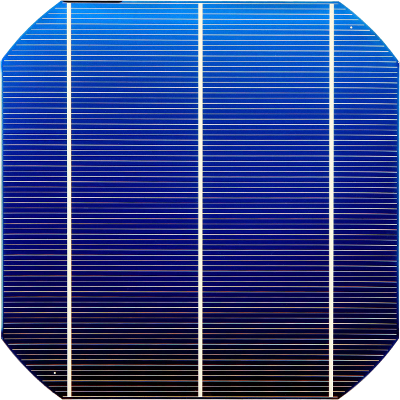
\includegraphics[width=0.4\textwidth]{images/solar-facility/cell--400px.png}
    \caption{Solarzelle, Frontalansicht \cite{ref:pvcell:wikipedia}}
    \label{fig:pvcell:front}
\end{wrapfigure}

Die   Grundbausteine    einer   Photovoltaikanlage   legen    die   PV-Zellen,
welche   aus   verschiedenen   Halbleitermaterialien   bestehen. Die   meisten
heutzutage  verwendeten  Zellen  werden aus  dem  Halbleitermaterial  Silizium
hergestellt. Siliziumzellen  sind in  verschiedenen Formfaktoren  verf\"ugbar;
g\"angige   Gr\"ossen    haben   ca.   zwischen    \SI{10}{\centi\meter}   und
\SI{15}{\centi\meter}  Kantenl\"ange.   Zum  mechanischen  Schutz  der  Zellen
sind  diese mit  einer durchsichtigen  Antireflexschicht \"uberzogen.   Die an
der  PV-Zelle  abgreifbare  Spannung betr\"agt  zwischen  \SI{0.5}{\volt}  und
\SI{0.8}{\volt} DC,  wobei die  Klemmenspannung einer  voll funktionsf\"ahigen
Zelle nur schwach von  der Lichteinstrahlung abh\"angig ist. Die Stromst\"arke
hingegen   ist  sehr   stark  von   der  Beleuchtungsst\"arke   abh\"angig. Je
nach    Sonneneinstrahlung   erreicht    eine   \SI{100}{\centi\meter\squared}
grosse   Siliziumzelle  eine   Stromst\"arke   von   bis  zu   \SI{2}{\ampere}
\cite{ref:pv:gesellschaftFuerSonnenenergie}. \fref{fig:pvcell:front} zeigt die
Frontansicht einer PV-Zelle.

\clearpage
\begin{wrapfigure}{l}{0.45\textwidth}
    \centering
    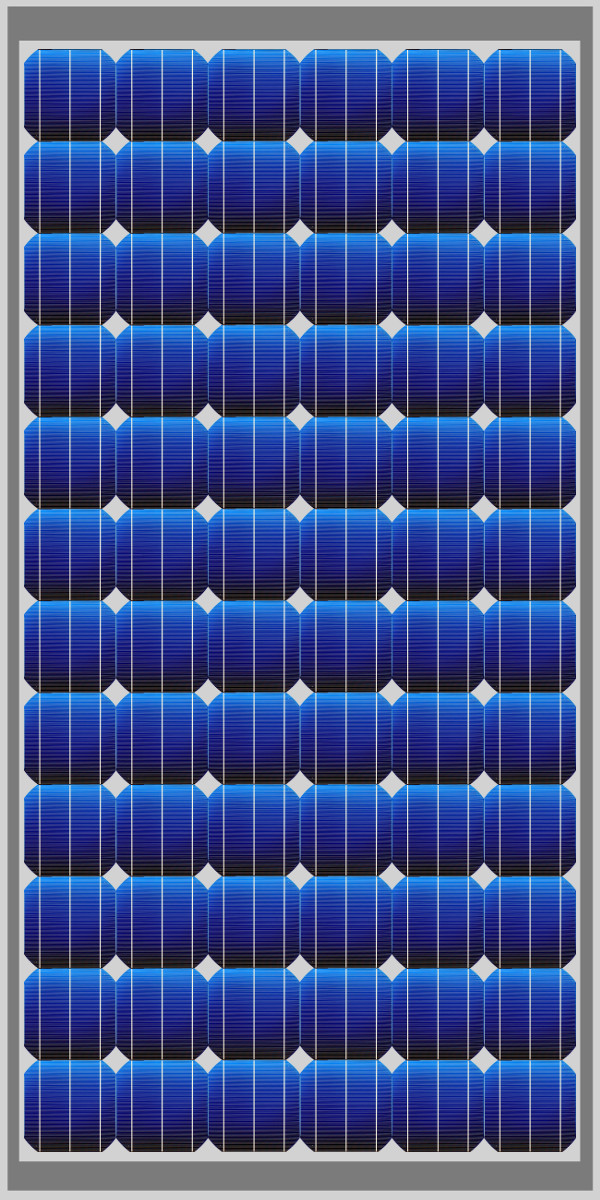
\includegraphics[width=0.4\textwidth]{images/solar-facility/pvmodule.jpeg}
    \caption{
        Solarmodul,  zusammengesetzt  aus  72 Solarzellen  gem\"ass  Abbildung
        \ref{fig:pvcell:front}%
    }
    \label{fig:pvmodule}
\end{wrapfigure}


Die  in der  Praxis  \"ubliche  Baugruppe ist  nicht  die Solarzelle,  sondern
das  Photovoltaikmodul.  Um  die Ausgangsspannung  und/oder den  Ausgangsstrom
zu  erh\"ohen  und um  diese  in  der  Praxis  besser einsetzen  zu  k\"onnen,
werden mehrere  Zellen in  verschiedenen Konfigurationen miteinander  zu einem
PV-Modul  verschaltet. Das Konzept  ist schematisch  dargestellt in  Abbildung
\ref{fig:pvmodule}, die Eckdaten einiger PV-Module  sind als Beispiele sind in
Anhang \ref{app:commercial:modules}  ab Seite \pageref{app:commercial:modules}
aufgef\"uhrt.

Zur  Erh\"ohung  des Ausgangsstroms  werden  Zellen  parallel geschaltet,  zur
Erh\"ohung  der  Ausgangsspannung werden  sie  in  Serie verbunden.   Je  nach
gew\"unschten Spezifikationen eines Moduls werden diese Ans\"atze einzeln oder
kombiniert angewandt.  In der Praxis \"ublich  sind Module mit 36, 72 oder 144
Zellen und  einer Ausgangsspannung  von \SI{12}{\volt}  bis \SI{60}{\volt}. In
Photovoltaikanlagen werden nur solche  ganzen Module eingesetzt; die einzelnen
Zellen  sind  f\"ur  Reparaturen  nicht  mehr  zug\"anglich. Die  elektrischen
Anschl\"usse befinden sich in kleinen  Kunststoffdosen auf der R\"uckseite der
Module (Beispiel in Abbildung \ref{fig:pvJunctionBox}) \cite{ref:pv:baunetz}.


Mehrere  identische  Module  werden  \"ublicherweise  mittels  Reihenschaltung
zu\hfill  einem\hfill  Modulstrang\hfill verschaltet\hfill  (vereinfacht\hfill
dargestellt\hfill in\hfill Abbildung\hfill \ref{fig:pvarray:gak:inverter}).

\begin{wrapfigure}{r}{0.35\textwidth}
    \centering
    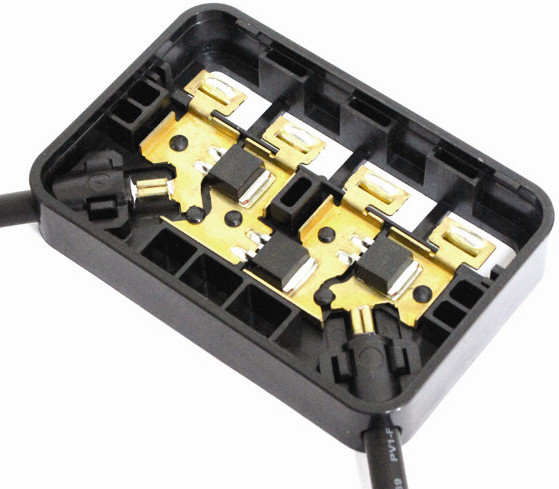
\includegraphics[width=0.3\textwidth]{images/solar-facility/pvJunctionBox.jpeg}
    \caption{
        Anschlussbox f\"ur Solarmodul, wird  normalerweise auf der R\"uckseite
        des Moduls montiert. \cite{ref:junctionBox}%
    }
    \label{fig:pvJunctionBox}
\end{wrapfigure}

\noindent  Dadurch  wird  eine  h\"ohere  Ausgangsspannung  erzeugt,  was  die
Umwandlung  des  Gleichstroms  in  Wechselstrom  und  dessen  Einspeisung  ins
Wechselstromnetz  erleichtert. Die  Ausgangsspannung eines  Modulstrangs  darf
gem\"ass Vorschrift \SI{1000}{\volt} DC  nicht \"uberschreiten, was die Anzahl
der in  einem Strang in  Serie geschalteten Module beschr\"ankt.   Module, die
an  unterschiedlichen Dachneigungen  montiert sind  oder die  unterschiedliche
Ausrichtungen  haben,  sollten  nie zu  einem  Modulstrang  zusammengeschaltet
werden, da sie nicht den gleichen  Strom produzieren werden, was die Effizienz
des Strangs stark reduziert. Ein einzelnes beschattetes oder nicht einwandfrei
funktionierendes   Modul  beeintr\"achtigt   die   vom  gesamten   Modulstrang
abgegebene Leistung stark (siehe auch n\"achster Abschnitt).

\begin{figure}[h!t]
    \centering
    \begin{tikzpicture}
        \begin{scope}[x={(0mm,\textwidth)},y={(0mm,-70mm)}]
            \node[inner sep=0pt,anchor=north west] at (0mm,0mm) {%
                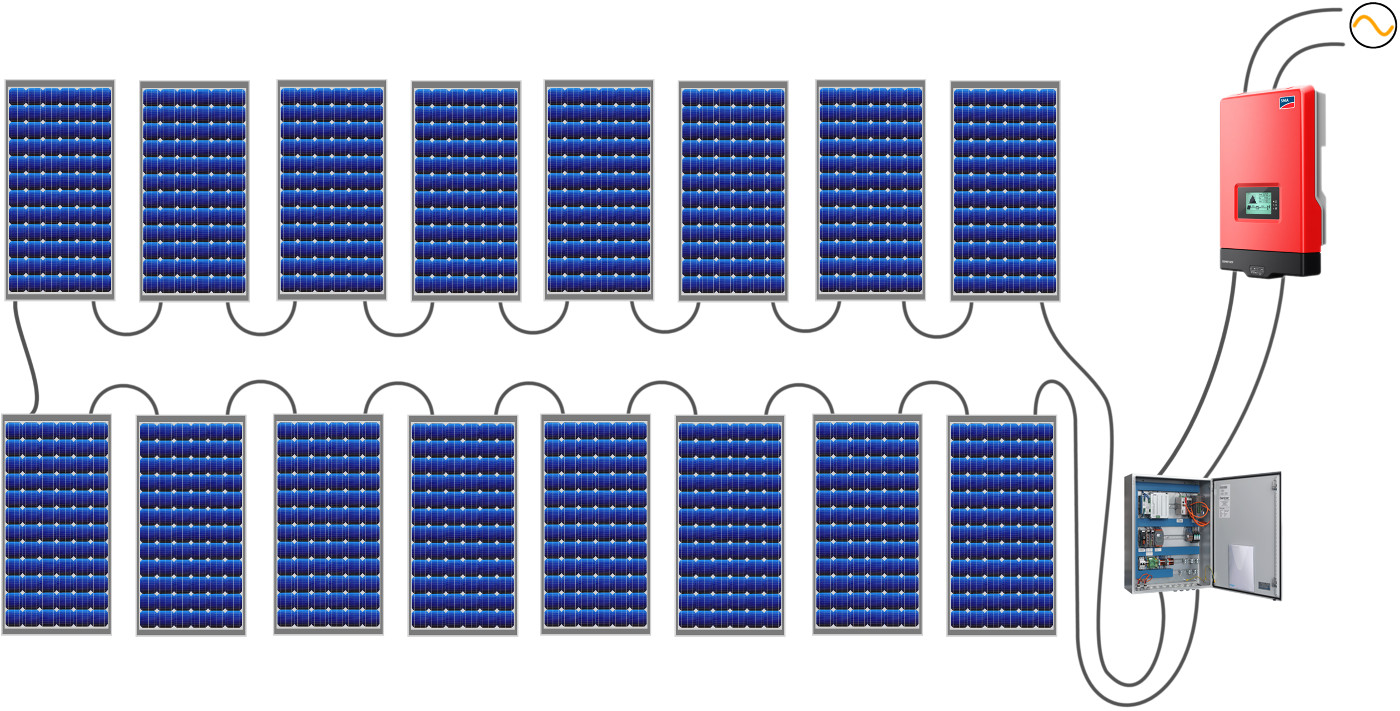
\includegraphics[width=\textwidth]{images/solar-facility/pvarray.jpeg}%
            };
            \node at (132mm,-55mm) {\small{GAK}};
            \node at (120mm,0mm) {\small{Wechselrichter}};
            \node at (55mm,-5mm) {\small{Modulstrang}};
        \end{scope}
    \end{tikzpicture}
    \caption{%
        Modulstrang aus 16 Modulen  gem\"ass Abbildung \ref{fig:pvmodule}, GAK
        und Wechselrichter. Bild des GAK  von \cite{ref:gak:gantner}, Bild des
        Wechselrichters von \cite{ref:inverter:sunnyboy}.%
    }
    \label{fig:pvarray:gak:inverter}
\end{figure}

Die    Umwandlung    der    Gleichspannung    in    Wechselspannung    erfolgt
mittels    Wechselrichter   (dargestellt    auf   der    rechten   Seite    in
Abbildung    \ref{fig:pvarray:gak:inverter}). Je     nach    Anwendungsbereich
werden  unterschiedliche  Wechselrichter  eingesetzt:\todo{Anwendungsbereiche,
Vor-Nachteile spezifizieren}

\begin{symbols}
    \firmlist
    \item[\textbf{Modulwechselrichter}:]
        Ein  Wechselrichter,  welcher  den  Strom eines  einzelnen  Moduls  in
        Wechselstrom konvertiert.
    \item[\textbf{Strangwechselrichter}:]
        Konvertiert den Strom eines Modulstrangs zu Wechselstrom.
    \item[\textbf{Multistrangwechselrichter}:]
        Fasst   die   Gleichstr\"ome   mehrer  Modulstr\"ange   zusammen   und
        konvertiert diese zu Wechselstrom.
    \item[\textbf{Zentralwechselrichter}:]
        Ein  einzelner Wechselrichter,  welcher den  Gleichstrom einer  ganzen
        Photovoltaikanlage in Wechselstrom umwandelt. Kommt haupts\"achlich in
        Grossanlagen zum Einsatz, bei denen alle Str\"ange die gleiche Neigung
        aufweisen und gleich ausgerichtet sind \cite{ref:pv:ratgeber}.
\end{symbols}

Als Leitungsschutz gegen \"Uberstrom und Kurzschluss befindet sich unmittelbar
vor  dem   Wechselrichter  im  Gleichstromnetz   ein  Generatoranschlusskasten
(GAK). Dieser   dient   auch   zur    Trennung   der   gesamten   Anlage   vom
Netz. \"Ublicherweise  werden  GAK  und   Wechselrichter  am  selben  Standort
platziert.


% ---------------------------------------------------------------------------- %
\clearpage
\section{Leistungseinbr\"uche}
\label{sec:shadedCells}
% ---------------------------------------------------------------------------- %

\todo{Referenzen auf Simu-Circuits}

% ---------------------------------------------------------------------------- %
% Performance Calculations
%
% Based on:
% http://tex.stackexchange.com/questions/185488/pgfplots-read-data-calculate-diagram#186016
% see also p56 of pgfplotstable manual:
% http://pgfplots.sourceforge.net/pgfplotstable.pdf
% ---------------------------------------------------------------------------- %

% \IfFileExists{./filename}{true branch}{false branch}
% NOTE: without the preceding './', \IfFileExists will check the entire tex path

\IfFileExists{./data/iv-curves/module-72cells-series--reference--all-ok--power.dat}
    { }
    {
        \pgfplotstablesave[
            create on use/power output/.style={create col/expr={\thisrow{V(out)} * \thisrow{I(R_load)}}},
            columns={V(out),power output},
        ]
            {data/iv-curves/module-72cells-series--reference--all-ok.dat}
            {data/iv-curves/module-72cells-series--reference--all-ok--power.dat}
    }

\IfFileExists{./data/iv-curves/module-72cells-series--reference--ifail-5A--power.dat}
    { }
    {
        \pgfplotstablesave[
            create on use/power output/.style={create col/expr={\thisrow{V(out)} * \thisrow{I(R_load)}}},
            columns={V(out),power output},
        ]
            {data/iv-curves/module-72cells-series--reference--ifail-5A.dat}
            {data/iv-curves/module-72cells-series--reference--ifail-5A--power.dat}
    }
\IfFileExists{./data/iv-curves/module-72cells-series--reference--ifail-1A--power.dat}
    { }
    {
        \pgfplotstablesave[
            create on use/power output/.style={create col/expr={\thisrow{V(out)} * \thisrow{I(R_load)}}},
            columns={V(out),power output},
        ]
            {data/iv-curves/module-72cells-series--reference--ifail-1A.dat}
            {data/iv-curves/module-72cells-series--reference--ifail-1A--power.dat}
    }
\IfFileExists{./data/iv-curves/module-string-complete--all-ok--power.dat}
    { }
    {
        \pgfplotstablesave[
            create on use/power output/.style={create col/expr={\thisrow{V(out)} * \thisrow{I(R_load)}}},
            columns={V(out),power output},
        ]
            {data/iv-curves/module-string-complete--all-ok.dat}
            {data/iv-curves/module-string-complete--all-ok--power.dat}
    }
\IfFileExists{./data/iv-curves/module-string-complete--ifail-5A--power.dat}
    { }
    {
        \pgfplotstablesave[
            create on use/power output/.style={create col/expr={\thisrow{V(out)} * \thisrow{I(R_load)}}},
            columns={V(out),power output},
        ]
            {data/iv-curves/module-string-complete--ifail-5A.dat}
            {data/iv-curves/module-string-complete--ifail-5A--power.dat}
    }
\IfFileExists{./data/iv-curves/module-string-complete--ifail-1A--power.dat}
    { }
    {
        \pgfplotstablesave[
            create on use/power output/.style={create col/expr={\thisrow{V(out)} * \thisrow{I(R_load)}}},
            columns={V(out),power output},
        ]
            {data/iv-curves/module-string-complete--ifail-1A.dat}
            {data/iv-curves/module-string-complete--ifail-1A--power.dat}
    }


\begin{figure}[h!tb]
    %\begin{tikzpicture}
%   \begin{scope}[x={(0mm,0mm)},y={(90mm,\textwidth)}]
%       \begin{axis}[%
%               height=50mm,
%               width=\textwidth,
%               at={(0,50mm)},
%               grid=both,
%               xlabel=Spannung (\si{\volt}),
%               ylabel=Strom (\si{\ampere}),
%               %axis y line*=left,
%               %x unit=u,
%               %change x base=true,
%               %line width = 1pt,
%               %thick,
%               %x SI prefix=micro,
%           ]
%            \addplot[-,color=blue] table {data/iv-curves/module-72cells-series--reference--all-ok.dat};
%            \addplot[-,color=teal] table {data/iv-curves/module-72cells-series--reference--ifail-5A.dat};
%            \addplot[-,color=magenta] table {data/iv-curves/module-72cells-series--reference--ifail-1A.dat};
%        \end{axis}
%        \begin{axis}[%
%               height=50mm,
%               width=\textwidth,
%               at={(0,0)},
%               grid=both,
%               xlabel=Spannung (\si{\volt}),
%               ylabel=Leistung (\si{\watt}),
%               %axis y line*=left,
%               %x unit=u,
%               %change x base=true,
%               %line width = 1pt,
%               %thick,
%               %x SI prefix=micro,
%           ]
%%            \addplot [blue] table [y=power output] {\cellsAllOK} node {};
%%            \addplot [teal] table [y=power output] {\cellsFiveA} node {};
%%            \addplot [magenta] table [y=power output] {\cellsOneA} node {};
%            \addplot[-,color=blue] table {data/iv-curves/module-72cells-series--reference--all-ok--power.dat};
%            \addplot[-,color=teal] table {data/iv-curves/module-72cells-series--reference--ifail-5A--power.dat};
%            \addplot[-,color=magenta] table {data/iv-curves/module-72cells-series--reference--ifail-1A--power.dat};
%        \end{axis}
%    \end{scope}
%\end{tikzpicture}

    \caption{%
        Oberes Diagramm: Simulierte  Strom-Spannungs-Kurve eines Moduls  aus 72
        Zellen (in Serie geschaltet) mit einer degradierten Zelle\protect\\
        Unteres Diagramm: Die zum oberen Diagramm geh\"orenden Leistungskurven.
        Gut erkennbar  ist, dass  selbst bei nur  einer degradierten  Zelle die
        verf\"ugbare Leistung des gesamten Moduls stark abnimmt.\protect\\
        \textbf{\textcolor{blue}{blau}}: Alle   Zellen  geben   volle  Leistung
        ab.\protect\\
        \textbf{\textcolor{teal}{blaugr\"un}}: Eine Zelle  von 72 gibt  nur den
        halben Strom ab.\protect\\
        \textbf{\textcolor{magenta}{magenta}}: Eine  Zelle  gibt nur  10\%  des
        vollen Stromes ab.\protect\\
        Die zuge\"orige \code{LTspice}-Schaltung basiert  auf dem Modell eines
        Moduls aus Abbildung \ref{fig:ltspice:module:cellBased:72x1} auf Seite
        \pageref{fig:ltspice:module:cellBased:72x1} im Anhang. Dabei wurde die
        Stromquelle  in  einer  Zelle  variiert  (100\%,  50\%  bzw. 10\%  der
        restlichen Quellen).%
    }
    \label{fig:ivcurve:cells}
\end{figure}
\begin{figure}[h!tb]
    \begin{tikzpicture}
   \begin{scope}[x={(0mm,0mm)},y={(100mm,\textwidth)}]
       \begin{axis}[%
               height=50mm,
               width=\textwidth,
               at={(0,50mm)},
               grid=both,
               xlabel=Spannung (\si{\volt}),
               ylabel=Strom (\si{\ampere}),
               %x unit=u,
               %change x base=true,
               %line width = 1pt,
               %thick,
               %x SI prefix=micro,
           ]
            \addplot[-,color=blue] table {data/iv-curves/module-string-complete--all-ok.dat};
            \addplot[-,color=magenta] table {data/iv-curves/module-string-complete--ifail-1A.dat};
            \addplot[-,color=teal] table {data/iv-curves/module-string-complete--ifail-5A.dat};
        \end{axis}
        \begin{axis}[%
               height=50mm,
               width=\textwidth,
               at={(0,0)},
               grid=both,
               xlabel=Spannung (\si{\volt}),
               ylabel=Leistung (\si{\watt}),
               %axis y line*=left,
               %x unit=u,
               %change x base=true,
               %line width = 1pt,
               %thick,
               %x SI prefix=micro,
           ]
            %\addplot [blue] table [y=power output] {\moduleAllOK} node {};
            %\addplot [teal] table [y=power output] {\moduleFiveA} node {};
            %\addplot [magenta] table [y=power output] {\moduleOneA} node {};
            \addplot[-,color=blue] table {data/iv-curves/module-string-complete--all-ok--power.dat};
            \addplot[-,color=magenta] table {data/iv-curves/module-string-complete--ifail-1A--power.dat};
            \addplot[-,color=teal] table {data/iv-curves/module-string-complete--ifail-5A--power.dat};
        \end{axis}
    \end{scope}
\end{tikzpicture}

    \caption{%
        Oberes   Diagramm: Simulierte   Strom-Spannungs-Kurve  eines   Strangs
        von   Modulen   mit   einem  degradierten   Modul.\protect\\   Unteres
        Diagramm: Die  zum   oberen  Diagramm   geh\"orenden  Leistungskurven.
        Selbst   ein   einzelnes   degradiertes   Modul   f\"uhrt   zu   einem
        bedeutenden Leistungseinbruch des  gesamten Modulstrangs.  Verkn\"upft
        man   diese   Erkenntnis   mit   den   Informationen   aus   Abbildung
        \ref{fig:ivcurve:cells},  l\"asst sich  folgern,  dass lediglich  eine
        einzelne degradierte  Zelle von mehreren hundert  in einem Modulstrang
        vorhandenen Zellen  die gesamte  auf dem Strang  verf\"ugbare Leistung
        massiv senken kann.\protect\\
        \textbf{\textcolor{blue}{blau}}: Alle   Module   geben  vollen   Strom
        ab.\protect\\
        \textbf{\textcolor{teal}{blaugr\"un}}: Ein Modul von  zwanzig gibt nur
        den halben Strom ab.\protect\\
        \textbf{\textcolor{magenta}{magenta}}: Ein  Modul  gibt nur  10\%  des
        vollen Stromes ab.\protect\\
        Die       zuge\"orige       \code{LTspice}-Schaltung      ist       in
        Abbildung    \ref{fig:ltspice:vicurvesimulator:modules}   auf    Seite
        \pageref{fig:ltspice:vicurvesimulator:modules} im Anhang zu finden.%
    }
    \label{fig:ivcurve:modules}
\end{figure}


% ---------------------------------------------------------------------------- %
\clearpage
\section{Unser System}
\label{sec:ourSystem}
% ---------------------------------------------------------------------------- %

Unser   System  bietet   neben   einer   benutzerfreundlichen  Bedienung   und
Inbetriebnahme,  so wie  einer  einfachen Integration  in bestehende  Anlagen,
ebenfalls  eine  kosteng\"unstige  und energieeffiziente  L\"osung  f\"ur  die
\"Uberwachung von Photovoltaikanlagen. Das System setzt sich zusammen aus zwei
Hauptkomponenten, dem Master-Ger\"at und den jeweiligen Sensoren.

Die Installation  des Master-Ger\"ates erfolgt im  zugeh\"origen Schaltschrank
des  Wechselrichters. Das  schlichte  Hutschienengeh\"ause  erm\"oglicht  eine
einfache   Installation   in   bestehende  oder   neue   Schaltschr\"anke. Die
Energieversorgung,  wie  auch  die  Ankopplung  an  die  DC-Leitungen  erfolgt
intern   des   Schaltschrankes   und  wird   von   einem   Elektroinstallateur
ausgef\"uhrt. Neben dem  Klemmenanschluss f\"ur die Energieversorgung  und den
zwei Relaisausg\"angen  f\"ur externe Alarmger\"ate, sieht  das Master-Ger\"at
die  Ankopplung  der  DC-Leitungen  von  bis  zu  drei  Modulstrangs  vor. Ein
internes 3.5“ Touch-Display erm\"oglicht eine einfache Inbetriebnahme und eine
benutzerfreundliche  Bedienung des  Systems. Alle  Messresultate der  Sensoren
werden  vom Master-Ger\"at  ausgewertet  und dem  Kunden  in einer  grafischen
Benutzeroberfl\"ache  dargestellt. Tritt ein  Fehler an  der Anlage  auf, wird
eine entsprechende Meldung auf dem Display angezeigt, die beiden Relais werden
bet\"atigt  und  eine  Nachricht  mittels  SMS  wird  versendet. Dadurch  wird
sichergestellt, dass der Kunde m\"oglichst schnell \"uber defekte PV-Module in
Kenntnis gesetzt wird.

Als Fehler werden folgende Ereignisse definiert:
\begin{itemize}
    \firmlist
    \item
        Eine defekte Zelle
    \item
        Eine dauerhaft verschmutzte Zelle
    \item
        Eine defekte Leitung
\end{itemize}

Kein Fehler soll in folgenden Situationen ausgel\"ost werden.
\begin{itemize}
    \firmlist
    \item
        Kurzzeitige Abschattungen (z.B. Vogel auf Zelle)
    \item
        Regelm\"assige Abschattungen,  die zu den  Umweltbedingungen geh\"oren
        (z.B. Baum, der t\"aglich abschattet)
    \item
        Nacht-/Schlechtwetter
    \item
        Anlage absichtlich ausser Betrieb genommen (z.B. Unterhaltsarbeiten)
\end{itemize}

F\"ur  die  Spannungsmessung  und  die \"Ubertragung  der  Messresultate  sind
die  Sensoren  zust\"andig. Die  Installation  der  Sensoren  erfolgt  in  den
Anschlussdosen  auf der  R\"uckseite der  PV-Module. F\"ur jedes  PV-Modul ist
jeweils  ein  Sensor  zu  installieren. Eine  zweiadrige  Verbindung  von  der
Sensorplatine  zu den  Klemmen  der Anschlussdose  ist  zust\"andig f\"ur  die
Energieversorgung des Sensors und die  Ankopplung an die DC-Leitung, f\"ur die
\"Ubertragung der Messresultate an das Master-Ger\"at.

% ---------------------------------------------------------------------------- %
\clearpage
\section{Kommunikation \"uber DC-Leitung}
\label{sec:commDCLine}
% ---------------------------------------------------------------------------- %

Die Kommunikation zwischen  \Sensor und \Master \"uber die  DC-Leitung ist das
Herzst\"uck des Systems und das zu l\"osende Kernproblem des Projekts. Es sind
im Rahmen  des Projekts  zwei grunds\"atzliche  Ans\"atze verfolgt  worden, um
Daten  zwischen  \Sensor und  \Master  \"uber  die  DC-Leitung zu  senden  und
empfangen.

\textbf{Frequency-shift keying}: Bei  der FSK (Frequenzumtastung  auf Deutsch)
wird  dem in  der Leitung  fliessenden Gleichstrom  ein (verh\"altnism\"assig)
kleines  Signal aufmoduliert,  welches  die  zu \"ubertragenden  Informationen
enth\"alt. Die  Frequenz   des  aufmodulierten   Anteils  wird   in  diskreten
Schritten variiert  und jeweils  einem Symbol zugeordnet. Bei  einer bin\"aren
Umsetzung  werden  zwei  Frequenzen  benutzt; eine  f\"ur  \code{0}  und  eine
f\"ur  \code{1}.   Das  Verfahren ist  schematisch  in  \fref{fig:fsk:concept}
dargestellt.

\begin{figure}[h!tb]
    \centering
    %% Creator: Matplotlib, PGF backend
%%
%% To include the figure in your LaTeX document, write
%%   \input{<filename>.pgf}
%%
%% Make sure the required packages are loaded in your preamble
%%   \usepackage{pgf}
%%
%% Figures using additional raster images can only be included by \input if
%% they are in the same directory as the main LaTeX file. For loading figures
%% from other directories you can use the `import` package
%%   \usepackage{import}
%% and then include the figures with
%%   \import{<path to file>}{<filename>.pgf}
%%
%% Matplotlib used the following preamble
%%   \usepackage{fontspec}
%%   \setmainfont{Bitstream Vera Serif}
%%   \setsansfont{Bitstream Vera Sans}
%%   \setmonofont{Bitstream Vera Sans Mono}
%%
\begingroup%
\makeatletter%
\begin{pgfpicture}%
\pgfpathrectangle{\pgfpointorigin}{\pgfqpoint{5.000000in}{3.500000in}}%
\pgfusepath{use as bounding box, clip}%
\begin{pgfscope}%
\pgfsetbuttcap%
\pgfsetmiterjoin%
\pgfsetlinewidth{0.000000pt}%
\definecolor{currentstroke}{rgb}{0.000000,0.000000,0.000000}%
\pgfsetstrokecolor{currentstroke}%
\pgfsetstrokeopacity{0.000000}%
\pgfsetdash{}{0pt}%
\pgfpathmoveto{\pgfqpoint{0.000000in}{0.000000in}}%
\pgfpathlineto{\pgfqpoint{5.000000in}{0.000000in}}%
\pgfpathlineto{\pgfqpoint{5.000000in}{3.500000in}}%
\pgfpathlineto{\pgfqpoint{0.000000in}{3.500000in}}%
\pgfpathclose%
\pgfusepath{}%
\end{pgfscope}%
\begin{pgfscope}%
\pgfsetbuttcap%
\pgfsetmiterjoin%
\pgfsetlinewidth{0.000000pt}%
\definecolor{currentstroke}{rgb}{0.000000,0.000000,0.000000}%
\pgfsetstrokecolor{currentstroke}%
\pgfsetstrokeopacity{0.000000}%
\pgfsetdash{}{0pt}%
\pgfpathmoveto{\pgfqpoint{0.750000in}{2.268396in}}%
\pgfpathlineto{\pgfqpoint{4.750000in}{2.268396in}}%
\pgfpathlineto{\pgfqpoint{4.750000in}{3.325000in}}%
\pgfpathlineto{\pgfqpoint{0.750000in}{3.325000in}}%
\pgfpathclose%
\pgfusepath{}%
\end{pgfscope}%
\begin{pgfscope}%
\pgfpathrectangle{\pgfqpoint{0.750000in}{2.268396in}}{\pgfqpoint{4.000000in}{1.056604in}} %
\pgfusepath{clip}%
\pgfsetrectcap%
\pgfsetroundjoin%
\pgfsetlinewidth{0.501875pt}%
\definecolor{currentstroke}{rgb}{0.000000,0.000000,1.000000}%
\pgfsetstrokecolor{currentstroke}%
\pgfsetdash{}{0pt}%
\pgfpathmoveto{\pgfqpoint{0.750000in}{2.356447in}}%
\pgfpathlineto{\pgfqpoint{1.701998in}{2.356447in}}%
\pgfusepath{stroke}%
\end{pgfscope}%
\begin{pgfscope}%
\pgfpathrectangle{\pgfqpoint{0.750000in}{2.268396in}}{\pgfqpoint{4.000000in}{1.056604in}} %
\pgfusepath{clip}%
\pgfsetrectcap%
\pgfsetroundjoin%
\pgfsetlinewidth{0.501875pt}%
\definecolor{currentstroke}{rgb}{0.501961,0.501961,0.501961}%
\pgfsetstrokecolor{currentstroke}%
\pgfsetdash{}{0pt}%
\pgfpathmoveto{\pgfqpoint{1.701998in}{2.356447in}}%
\pgfpathlineto{\pgfqpoint{1.701998in}{3.236950in}}%
\pgfusepath{stroke}%
\end{pgfscope}%
\begin{pgfscope}%
\pgfpathrectangle{\pgfqpoint{0.750000in}{2.268396in}}{\pgfqpoint{4.000000in}{1.056604in}} %
\pgfusepath{clip}%
\pgfsetrectcap%
\pgfsetroundjoin%
\pgfsetlinewidth{0.501875pt}%
\definecolor{currentstroke}{rgb}{1.000000,0.000000,1.000000}%
\pgfsetstrokecolor{currentstroke}%
\pgfsetdash{}{0pt}%
\pgfpathmoveto{\pgfqpoint{1.701998in}{3.236950in}}%
\pgfpathlineto{\pgfqpoint{2.653996in}{3.236950in}}%
\pgfusepath{stroke}%
\end{pgfscope}%
\begin{pgfscope}%
\pgfpathrectangle{\pgfqpoint{0.750000in}{2.268396in}}{\pgfqpoint{4.000000in}{1.056604in}} %
\pgfusepath{clip}%
\pgfsetrectcap%
\pgfsetroundjoin%
\pgfsetlinewidth{0.501875pt}%
\definecolor{currentstroke}{rgb}{0.501961,0.501961,0.501961}%
\pgfsetstrokecolor{currentstroke}%
\pgfsetdash{}{0pt}%
\pgfpathmoveto{\pgfqpoint{2.653996in}{3.236950in}}%
\pgfpathlineto{\pgfqpoint{2.653996in}{2.356447in}}%
\pgfusepath{stroke}%
\end{pgfscope}%
\begin{pgfscope}%
\pgfpathrectangle{\pgfqpoint{0.750000in}{2.268396in}}{\pgfqpoint{4.000000in}{1.056604in}} %
\pgfusepath{clip}%
\pgfsetrectcap%
\pgfsetroundjoin%
\pgfsetlinewidth{0.501875pt}%
\definecolor{currentstroke}{rgb}{0.000000,0.000000,1.000000}%
\pgfsetstrokecolor{currentstroke}%
\pgfsetdash{}{0pt}%
\pgfpathmoveto{\pgfqpoint{2.653996in}{2.356447in}}%
\pgfpathlineto{\pgfqpoint{3.605993in}{2.356447in}}%
\pgfusepath{stroke}%
\end{pgfscope}%
\begin{pgfscope}%
\pgfpathrectangle{\pgfqpoint{0.750000in}{2.268396in}}{\pgfqpoint{4.000000in}{1.056604in}} %
\pgfusepath{clip}%
\pgfsetrectcap%
\pgfsetroundjoin%
\pgfsetlinewidth{0.501875pt}%
\definecolor{currentstroke}{rgb}{0.501961,0.501961,0.501961}%
\pgfsetstrokecolor{currentstroke}%
\pgfsetdash{}{0pt}%
\pgfpathmoveto{\pgfqpoint{3.605993in}{2.356447in}}%
\pgfpathlineto{\pgfqpoint{3.605993in}{3.236950in}}%
\pgfusepath{stroke}%
\end{pgfscope}%
\begin{pgfscope}%
\pgfpathrectangle{\pgfqpoint{0.750000in}{2.268396in}}{\pgfqpoint{4.000000in}{1.056604in}} %
\pgfusepath{clip}%
\pgfsetrectcap%
\pgfsetroundjoin%
\pgfsetlinewidth{0.501875pt}%
\definecolor{currentstroke}{rgb}{1.000000,0.000000,1.000000}%
\pgfsetstrokecolor{currentstroke}%
\pgfsetdash{}{0pt}%
\pgfpathmoveto{\pgfqpoint{3.605993in}{3.236950in}}%
\pgfpathlineto{\pgfqpoint{4.557991in}{3.236950in}}%
\pgfusepath{stroke}%
\end{pgfscope}%
\begin{pgfscope}%
\pgfsetrectcap%
\pgfsetmiterjoin%
\pgfsetlinewidth{0.501875pt}%
\definecolor{currentstroke}{rgb}{0.000000,0.000000,0.000000}%
\pgfsetstrokecolor{currentstroke}%
\pgfsetdash{}{0pt}%
\pgfpathmoveto{\pgfqpoint{4.750000in}{2.268396in}}%
\pgfpathlineto{\pgfqpoint{4.750000in}{3.325000in}}%
\pgfusepath{stroke}%
\end{pgfscope}%
\begin{pgfscope}%
\pgfsetrectcap%
\pgfsetmiterjoin%
\pgfsetlinewidth{0.501875pt}%
\definecolor{currentstroke}{rgb}{0.000000,0.000000,0.000000}%
\pgfsetstrokecolor{currentstroke}%
\pgfsetdash{}{0pt}%
\pgfpathmoveto{\pgfqpoint{0.750000in}{3.325000in}}%
\pgfpathlineto{\pgfqpoint{4.750000in}{3.325000in}}%
\pgfusepath{stroke}%
\end{pgfscope}%
\begin{pgfscope}%
\pgfsetrectcap%
\pgfsetmiterjoin%
\pgfsetlinewidth{0.501875pt}%
\definecolor{currentstroke}{rgb}{0.000000,0.000000,0.000000}%
\pgfsetstrokecolor{currentstroke}%
\pgfsetdash{}{0pt}%
\pgfpathmoveto{\pgfqpoint{0.750000in}{2.268396in}}%
\pgfpathlineto{\pgfqpoint{4.750000in}{2.268396in}}%
\pgfusepath{stroke}%
\end{pgfscope}%
\begin{pgfscope}%
\pgfsetrectcap%
\pgfsetmiterjoin%
\pgfsetlinewidth{0.501875pt}%
\definecolor{currentstroke}{rgb}{0.000000,0.000000,0.000000}%
\pgfsetstrokecolor{currentstroke}%
\pgfsetdash{}{0pt}%
\pgfpathmoveto{\pgfqpoint{0.750000in}{2.268396in}}%
\pgfpathlineto{\pgfqpoint{0.750000in}{3.325000in}}%
\pgfusepath{stroke}%
\end{pgfscope}%
\begin{pgfscope}%
\pgftext[x=2.750000in,y=2.198952in,,top]{\rmfamily\fontsize{9.000000}{10.800000}\selectfont Zeit}%
\end{pgfscope}%
\begin{pgfscope}%
\pgfsetbuttcap%
\pgfsetroundjoin%
\definecolor{currentfill}{rgb}{0.000000,0.000000,0.000000}%
\pgfsetfillcolor{currentfill}%
\pgfsetlinewidth{0.501875pt}%
\definecolor{currentstroke}{rgb}{0.000000,0.000000,0.000000}%
\pgfsetstrokecolor{currentstroke}%
\pgfsetdash{}{0pt}%
\pgfsys@defobject{currentmarker}{\pgfqpoint{0.000000in}{0.000000in}}{\pgfqpoint{0.055556in}{0.000000in}}{%
\pgfpathmoveto{\pgfqpoint{0.000000in}{0.000000in}}%
\pgfpathlineto{\pgfqpoint{0.055556in}{0.000000in}}%
\pgfusepath{stroke,fill}%
}%
\begin{pgfscope}%
\pgfsys@transformshift{0.750000in}{2.356447in}%
\pgfsys@useobject{currentmarker}{}%
\end{pgfscope}%
\end{pgfscope}%
\begin{pgfscope}%
\pgfsetbuttcap%
\pgfsetroundjoin%
\definecolor{currentfill}{rgb}{0.000000,0.000000,0.000000}%
\pgfsetfillcolor{currentfill}%
\pgfsetlinewidth{0.501875pt}%
\definecolor{currentstroke}{rgb}{0.000000,0.000000,0.000000}%
\pgfsetstrokecolor{currentstroke}%
\pgfsetdash{}{0pt}%
\pgfsys@defobject{currentmarker}{\pgfqpoint{-0.055556in}{0.000000in}}{\pgfqpoint{0.000000in}{0.000000in}}{%
\pgfpathmoveto{\pgfqpoint{0.000000in}{0.000000in}}%
\pgfpathlineto{\pgfqpoint{-0.055556in}{0.000000in}}%
\pgfusepath{stroke,fill}%
}%
\begin{pgfscope}%
\pgfsys@transformshift{4.750000in}{2.356447in}%
\pgfsys@useobject{currentmarker}{}%
\end{pgfscope}%
\end{pgfscope}%
\begin{pgfscope}%
\pgftext[x=0.694444in,y=2.356447in,right,]{\rmfamily\fontsize{9.000000}{10.800000}\selectfont \(\displaystyle 0\)}%
\end{pgfscope}%
\begin{pgfscope}%
\pgfsetbuttcap%
\pgfsetroundjoin%
\definecolor{currentfill}{rgb}{0.000000,0.000000,0.000000}%
\pgfsetfillcolor{currentfill}%
\pgfsetlinewidth{0.501875pt}%
\definecolor{currentstroke}{rgb}{0.000000,0.000000,0.000000}%
\pgfsetstrokecolor{currentstroke}%
\pgfsetdash{}{0pt}%
\pgfsys@defobject{currentmarker}{\pgfqpoint{0.000000in}{0.000000in}}{\pgfqpoint{0.055556in}{0.000000in}}{%
\pgfpathmoveto{\pgfqpoint{0.000000in}{0.000000in}}%
\pgfpathlineto{\pgfqpoint{0.055556in}{0.000000in}}%
\pgfusepath{stroke,fill}%
}%
\begin{pgfscope}%
\pgfsys@transformshift{0.750000in}{3.236950in}%
\pgfsys@useobject{currentmarker}{}%
\end{pgfscope}%
\end{pgfscope}%
\begin{pgfscope}%
\pgfsetbuttcap%
\pgfsetroundjoin%
\definecolor{currentfill}{rgb}{0.000000,0.000000,0.000000}%
\pgfsetfillcolor{currentfill}%
\pgfsetlinewidth{0.501875pt}%
\definecolor{currentstroke}{rgb}{0.000000,0.000000,0.000000}%
\pgfsetstrokecolor{currentstroke}%
\pgfsetdash{}{0pt}%
\pgfsys@defobject{currentmarker}{\pgfqpoint{-0.055556in}{0.000000in}}{\pgfqpoint{0.000000in}{0.000000in}}{%
\pgfpathmoveto{\pgfqpoint{0.000000in}{0.000000in}}%
\pgfpathlineto{\pgfqpoint{-0.055556in}{0.000000in}}%
\pgfusepath{stroke,fill}%
}%
\begin{pgfscope}%
\pgfsys@transformshift{4.750000in}{3.236950in}%
\pgfsys@useobject{currentmarker}{}%
\end{pgfscope}%
\end{pgfscope}%
\begin{pgfscope}%
\pgftext[x=0.694444in,y=3.236950in,right,]{\rmfamily\fontsize{9.000000}{10.800000}\selectfont \(\displaystyle 1\)}%
\end{pgfscope}%
\begin{pgfscope}%
\pgftext[x=0.560764in,y=2.796698in,,bottom,rotate=90.000000]{\rmfamily\fontsize{9.000000}{10.800000}\selectfont Symbol}%
\end{pgfscope}%
\begin{pgfscope}%
\pgftext[x=2.750000in,y=3.394444in,,base]{\rmfamily\fontsize{11.000000}{13.200000}\selectfont Daten}%
\end{pgfscope}%
\begin{pgfscope}%
\pgfsetbuttcap%
\pgfsetmiterjoin%
\pgfsetlinewidth{0.000000pt}%
\definecolor{currentstroke}{rgb}{0.000000,0.000000,0.000000}%
\pgfsetstrokecolor{currentstroke}%
\pgfsetstrokeopacity{0.000000}%
\pgfsetdash{}{0pt}%
\pgfpathmoveto{\pgfqpoint{0.750000in}{0.525000in}}%
\pgfpathlineto{\pgfqpoint{4.750000in}{0.525000in}}%
\pgfpathlineto{\pgfqpoint{4.750000in}{1.581604in}}%
\pgfpathlineto{\pgfqpoint{0.750000in}{1.581604in}}%
\pgfpathclose%
\pgfusepath{}%
\end{pgfscope}%
\begin{pgfscope}%
\pgfpathrectangle{\pgfqpoint{0.750000in}{0.525000in}}{\pgfqpoint{4.000000in}{1.056604in}} %
\pgfusepath{clip}%
\pgfsetrectcap%
\pgfsetroundjoin%
\pgfsetlinewidth{0.501875pt}%
\definecolor{currentstroke}{rgb}{0.000000,0.000000,1.000000}%
\pgfsetstrokecolor{currentstroke}%
\pgfsetdash{}{0pt}%
\pgfpathmoveto{\pgfqpoint{0.750000in}{0.573027in}}%
\pgfpathlineto{\pgfqpoint{0.754765in}{0.573977in}}%
\pgfpathlineto{\pgfqpoint{0.760482in}{0.577618in}}%
\pgfpathlineto{\pgfqpoint{0.766200in}{0.583967in}}%
\pgfpathlineto{\pgfqpoint{0.772871in}{0.594748in}}%
\pgfpathlineto{\pgfqpoint{0.780494in}{0.611414in}}%
\pgfpathlineto{\pgfqpoint{0.789071in}{0.635497in}}%
\pgfpathlineto{\pgfqpoint{0.799553in}{0.672160in}}%
\pgfpathlineto{\pgfqpoint{0.810989in}{0.720437in}}%
\pgfpathlineto{\pgfqpoint{0.825283in}{0.791283in}}%
\pgfpathlineto{\pgfqpoint{0.842436in}{0.888329in}}%
\pgfpathlineto{\pgfqpoint{0.869119in}{1.054057in}}%
\pgfpathlineto{\pgfqpoint{0.902472in}{1.258667in}}%
\pgfpathlineto{\pgfqpoint{0.919625in}{1.350889in}}%
\pgfpathlineto{\pgfqpoint{0.933919in}{1.416314in}}%
\pgfpathlineto{\pgfqpoint{0.946308in}{1.462665in}}%
\pgfpathlineto{\pgfqpoint{0.956790in}{1.493395in}}%
\pgfpathlineto{\pgfqpoint{0.965367in}{1.512303in}}%
\pgfpathlineto{\pgfqpoint{0.972990in}{1.524182in}}%
\pgfpathlineto{\pgfqpoint{0.979661in}{1.530670in}}%
\pgfpathlineto{\pgfqpoint{0.985379in}{1.533289in}}%
\pgfpathlineto{\pgfqpoint{0.990144in}{1.533384in}}%
\pgfpathlineto{\pgfqpoint{0.994908in}{1.531581in}}%
\pgfpathlineto{\pgfqpoint{1.000626in}{1.526921in}}%
\pgfpathlineto{\pgfqpoint{1.007297in}{1.518079in}}%
\pgfpathlineto{\pgfqpoint{1.014920in}{1.503570in}}%
\pgfpathlineto{\pgfqpoint{1.023497in}{1.481811in}}%
\pgfpathlineto{\pgfqpoint{1.033026in}{1.451214in}}%
\pgfpathlineto{\pgfqpoint{1.044462in}{1.406247in}}%
\pgfpathlineto{\pgfqpoint{1.057803in}{1.343724in}}%
\pgfpathlineto{\pgfqpoint{1.074003in}{1.255932in}}%
\pgfpathlineto{\pgfqpoint{1.095921in}{1.123283in}}%
\pgfpathlineto{\pgfqpoint{1.144522in}{0.825031in}}%
\pgfpathlineto{\pgfqpoint{1.160722in}{0.740557in}}%
\pgfpathlineto{\pgfqpoint{1.174063in}{0.681536in}}%
\pgfpathlineto{\pgfqpoint{1.185498in}{0.640040in}}%
\pgfpathlineto{\pgfqpoint{1.195981in}{0.610239in}}%
\pgfpathlineto{\pgfqpoint{1.204557in}{0.592135in}}%
\pgfpathlineto{\pgfqpoint{1.212181in}{0.580994in}}%
\pgfpathlineto{\pgfqpoint{1.218852in}{0.575163in}}%
\pgfpathlineto{\pgfqpoint{1.224569in}{0.573113in}}%
\pgfpathlineto{\pgfqpoint{1.229334in}{0.573493in}}%
\pgfpathlineto{\pgfqpoint{1.235052in}{0.576453in}}%
\pgfpathlineto{\pgfqpoint{1.240770in}{0.582127in}}%
\pgfpathlineto{\pgfqpoint{1.247440in}{0.592135in}}%
\pgfpathlineto{\pgfqpoint{1.255064in}{0.607943in}}%
\pgfpathlineto{\pgfqpoint{1.263640in}{0.631102in}}%
\pgfpathlineto{\pgfqpoint{1.274123in}{0.666714in}}%
\pgfpathlineto{\pgfqpoint{1.285558in}{0.713964in}}%
\pgfpathlineto{\pgfqpoint{1.298900in}{0.778756in}}%
\pgfpathlineto{\pgfqpoint{1.316053in}{0.874228in}}%
\pgfpathlineto{\pgfqpoint{1.340829in}{1.026884in}}%
\pgfpathlineto{\pgfqpoint{1.378947in}{1.261394in}}%
\pgfpathlineto{\pgfqpoint{1.396101in}{1.353254in}}%
\pgfpathlineto{\pgfqpoint{1.410395in}{1.418285in}}%
\pgfpathlineto{\pgfqpoint{1.421830in}{1.461077in}}%
\pgfpathlineto{\pgfqpoint{1.432313in}{1.492177in}}%
\pgfpathlineto{\pgfqpoint{1.440889in}{1.511404in}}%
\pgfpathlineto{\pgfqpoint{1.448513in}{1.523578in}}%
\pgfpathlineto{\pgfqpoint{1.455184in}{1.530329in}}%
\pgfpathlineto{\pgfqpoint{1.460901in}{1.533175in}}%
\pgfpathlineto{\pgfqpoint{1.465666in}{1.533460in}}%
\pgfpathlineto{\pgfqpoint{1.470431in}{1.531846in}}%
\pgfpathlineto{\pgfqpoint{1.476148in}{1.527413in}}%
\pgfpathlineto{\pgfqpoint{1.482819in}{1.518831in}}%
\pgfpathlineto{\pgfqpoint{1.490443in}{1.504612in}}%
\pgfpathlineto{\pgfqpoint{1.499019in}{1.483167in}}%
\pgfpathlineto{\pgfqpoint{1.508549in}{1.452898in}}%
\pgfpathlineto{\pgfqpoint{1.519984in}{1.408289in}}%
\pgfpathlineto{\pgfqpoint{1.533325in}{1.346124in}}%
\pgfpathlineto{\pgfqpoint{1.549526in}{1.258667in}}%
\pgfpathlineto{\pgfqpoint{1.571444in}{1.126270in}}%
\pgfpathlineto{\pgfqpoint{1.620997in}{0.822378in}}%
\pgfpathlineto{\pgfqpoint{1.637197in}{0.738270in}}%
\pgfpathlineto{\pgfqpoint{1.650538in}{0.679631in}}%
\pgfpathlineto{\pgfqpoint{1.661974in}{0.638509in}}%
\pgfpathlineto{\pgfqpoint{1.671503in}{0.611414in}}%
\pgfpathlineto{\pgfqpoint{1.680080in}{0.592988in}}%
\pgfpathlineto{\pgfqpoint{1.687704in}{0.581551in}}%
\pgfpathlineto{\pgfqpoint{1.694374in}{0.575457in}}%
\pgfpathlineto{\pgfqpoint{1.700092in}{0.573179in}}%
\pgfpathlineto{\pgfqpoint{1.701998in}{0.573027in}}%
\pgfpathlineto{\pgfqpoint{1.701998in}{0.573027in}}%
\pgfusepath{stroke}%
\end{pgfscope}%
\begin{pgfscope}%
\pgfpathrectangle{\pgfqpoint{0.750000in}{0.525000in}}{\pgfqpoint{4.000000in}{1.056604in}} %
\pgfusepath{clip}%
\pgfsetrectcap%
\pgfsetroundjoin%
\pgfsetlinewidth{0.501875pt}%
\definecolor{currentstroke}{rgb}{1.000000,0.000000,1.000000}%
\pgfsetstrokecolor{currentstroke}%
\pgfsetdash{}{0pt}%
\pgfpathmoveto{\pgfqpoint{1.701998in}{0.573027in}}%
\pgfpathlineto{\pgfqpoint{1.703904in}{0.574395in}}%
\pgfpathlineto{\pgfqpoint{1.706763in}{0.581551in}}%
\pgfpathlineto{\pgfqpoint{1.710574in}{0.600462in}}%
\pgfpathlineto{\pgfqpoint{1.715339in}{0.638509in}}%
\pgfpathlineto{\pgfqpoint{1.721057in}{0.703445in}}%
\pgfpathlineto{\pgfqpoint{1.728680in}{0.817099in}}%
\pgfpathlineto{\pgfqpoint{1.741069in}{1.041975in}}%
\pgfpathlineto{\pgfqpoint{1.757269in}{1.331553in}}%
\pgfpathlineto{\pgfqpoint{1.765845in}{1.446069in}}%
\pgfpathlineto{\pgfqpoint{1.771563in}{1.498094in}}%
\pgfpathlineto{\pgfqpoint{1.776328in}{1.524182in}}%
\pgfpathlineto{\pgfqpoint{1.779187in}{1.531846in}}%
\pgfpathlineto{\pgfqpoint{1.781093in}{1.533555in}}%
\pgfpathlineto{\pgfqpoint{1.782999in}{1.532529in}}%
\pgfpathlineto{\pgfqpoint{1.785857in}{1.525881in}}%
\pgfpathlineto{\pgfqpoint{1.789669in}{1.507631in}}%
\pgfpathlineto{\pgfqpoint{1.794434in}{1.470360in}}%
\pgfpathlineto{\pgfqpoint{1.800152in}{1.406247in}}%
\pgfpathlineto{\pgfqpoint{1.807775in}{1.293439in}}%
\pgfpathlineto{\pgfqpoint{1.820164in}{1.069158in}}%
\pgfpathlineto{\pgfqpoint{1.837317in}{0.764085in}}%
\pgfpathlineto{\pgfqpoint{1.844940in}{0.663160in}}%
\pgfpathlineto{\pgfqpoint{1.850658in}{0.610239in}}%
\pgfpathlineto{\pgfqpoint{1.855423in}{0.583335in}}%
\pgfpathlineto{\pgfqpoint{1.859235in}{0.573797in}}%
\pgfpathlineto{\pgfqpoint{1.861141in}{0.573113in}}%
\pgfpathlineto{\pgfqpoint{1.863046in}{0.575163in}}%
\pgfpathlineto{\pgfqpoint{1.865905in}{0.583335in}}%
\pgfpathlineto{\pgfqpoint{1.869717in}{0.603561in}}%
\pgfpathlineto{\pgfqpoint{1.874482in}{0.643151in}}%
\pgfpathlineto{\pgfqpoint{1.880200in}{0.709715in}}%
\pgfpathlineto{\pgfqpoint{1.887823in}{0.825031in}}%
\pgfpathlineto{\pgfqpoint{1.901164in}{1.069158in}}%
\pgfpathlineto{\pgfqpoint{1.916412in}{1.338889in}}%
\pgfpathlineto{\pgfqpoint{1.924035in}{1.440784in}}%
\pgfpathlineto{\pgfqpoint{1.929753in}{1.494596in}}%
\pgfpathlineto{\pgfqpoint{1.934518in}{1.522314in}}%
\pgfpathlineto{\pgfqpoint{1.938330in}{1.532529in}}%
\pgfpathlineto{\pgfqpoint{1.940235in}{1.533555in}}%
\pgfpathlineto{\pgfqpoint{1.942141in}{1.531846in}}%
\pgfpathlineto{\pgfqpoint{1.945000in}{1.524182in}}%
\pgfpathlineto{\pgfqpoint{1.948812in}{1.504612in}}%
\pgfpathlineto{\pgfqpoint{1.953577in}{1.465792in}}%
\pgfpathlineto{\pgfqpoint{1.959294in}{1.400039in}}%
\pgfpathlineto{\pgfqpoint{1.966918in}{1.285549in}}%
\pgfpathlineto{\pgfqpoint{1.979306in}{1.060098in}}%
\pgfpathlineto{\pgfqpoint{1.995507in}{0.771370in}}%
\pgfpathlineto{\pgfqpoint{2.004083in}{0.657945in}}%
\pgfpathlineto{\pgfqpoint{2.009801in}{0.606821in}}%
\pgfpathlineto{\pgfqpoint{2.014566in}{0.581551in}}%
\pgfpathlineto{\pgfqpoint{2.017424in}{0.574395in}}%
\pgfpathlineto{\pgfqpoint{2.019330in}{0.573027in}}%
\pgfpathlineto{\pgfqpoint{2.021236in}{0.574395in}}%
\pgfpathlineto{\pgfqpoint{2.024095in}{0.581551in}}%
\pgfpathlineto{\pgfqpoint{2.027907in}{0.600462in}}%
\pgfpathlineto{\pgfqpoint{2.032672in}{0.638509in}}%
\pgfpathlineto{\pgfqpoint{2.038389in}{0.703445in}}%
\pgfpathlineto{\pgfqpoint{2.046013in}{0.817099in}}%
\pgfpathlineto{\pgfqpoint{2.058401in}{1.041975in}}%
\pgfpathlineto{\pgfqpoint{2.074602in}{1.331553in}}%
\pgfpathlineto{\pgfqpoint{2.083178in}{1.446069in}}%
\pgfpathlineto{\pgfqpoint{2.088896in}{1.498094in}}%
\pgfpathlineto{\pgfqpoint{2.093661in}{1.524182in}}%
\pgfpathlineto{\pgfqpoint{2.096519in}{1.531846in}}%
\pgfpathlineto{\pgfqpoint{2.098425in}{1.533555in}}%
\pgfpathlineto{\pgfqpoint{2.100331in}{1.532529in}}%
\pgfpathlineto{\pgfqpoint{2.103190in}{1.525881in}}%
\pgfpathlineto{\pgfqpoint{2.107002in}{1.507631in}}%
\pgfpathlineto{\pgfqpoint{2.111767in}{1.470360in}}%
\pgfpathlineto{\pgfqpoint{2.117484in}{1.406247in}}%
\pgfpathlineto{\pgfqpoint{2.125108in}{1.293439in}}%
\pgfpathlineto{\pgfqpoint{2.137496in}{1.069158in}}%
\pgfpathlineto{\pgfqpoint{2.154649in}{0.764085in}}%
\pgfpathlineto{\pgfqpoint{2.162273in}{0.663160in}}%
\pgfpathlineto{\pgfqpoint{2.167991in}{0.610239in}}%
\pgfpathlineto{\pgfqpoint{2.172755in}{0.583335in}}%
\pgfpathlineto{\pgfqpoint{2.176567in}{0.573797in}}%
\pgfpathlineto{\pgfqpoint{2.178473in}{0.573113in}}%
\pgfpathlineto{\pgfqpoint{2.180379in}{0.575163in}}%
\pgfpathlineto{\pgfqpoint{2.183238in}{0.583335in}}%
\pgfpathlineto{\pgfqpoint{2.187050in}{0.603561in}}%
\pgfpathlineto{\pgfqpoint{2.191814in}{0.643151in}}%
\pgfpathlineto{\pgfqpoint{2.197532in}{0.709715in}}%
\pgfpathlineto{\pgfqpoint{2.205156in}{0.825031in}}%
\pgfpathlineto{\pgfqpoint{2.218497in}{1.069158in}}%
\pgfpathlineto{\pgfqpoint{2.233744in}{1.338889in}}%
\pgfpathlineto{\pgfqpoint{2.241368in}{1.440784in}}%
\pgfpathlineto{\pgfqpoint{2.247086in}{1.494596in}}%
\pgfpathlineto{\pgfqpoint{2.251850in}{1.522314in}}%
\pgfpathlineto{\pgfqpoint{2.255662in}{1.532529in}}%
\pgfpathlineto{\pgfqpoint{2.257568in}{1.533555in}}%
\pgfpathlineto{\pgfqpoint{2.259474in}{1.531846in}}%
\pgfpathlineto{\pgfqpoint{2.262333in}{1.524182in}}%
\pgfpathlineto{\pgfqpoint{2.266145in}{1.504612in}}%
\pgfpathlineto{\pgfqpoint{2.270909in}{1.465792in}}%
\pgfpathlineto{\pgfqpoint{2.276627in}{1.400039in}}%
\pgfpathlineto{\pgfqpoint{2.284251in}{1.285549in}}%
\pgfpathlineto{\pgfqpoint{2.296639in}{1.060098in}}%
\pgfpathlineto{\pgfqpoint{2.312839in}{0.771370in}}%
\pgfpathlineto{\pgfqpoint{2.321416in}{0.657945in}}%
\pgfpathlineto{\pgfqpoint{2.327133in}{0.606821in}}%
\pgfpathlineto{\pgfqpoint{2.331898in}{0.581551in}}%
\pgfpathlineto{\pgfqpoint{2.334757in}{0.574395in}}%
\pgfpathlineto{\pgfqpoint{2.336663in}{0.573027in}}%
\pgfpathlineto{\pgfqpoint{2.338569in}{0.574395in}}%
\pgfpathlineto{\pgfqpoint{2.341428in}{0.581551in}}%
\pgfpathlineto{\pgfqpoint{2.345240in}{0.600462in}}%
\pgfpathlineto{\pgfqpoint{2.350004in}{0.638509in}}%
\pgfpathlineto{\pgfqpoint{2.355722in}{0.703445in}}%
\pgfpathlineto{\pgfqpoint{2.363346in}{0.817099in}}%
\pgfpathlineto{\pgfqpoint{2.375734in}{1.041975in}}%
\pgfpathlineto{\pgfqpoint{2.391934in}{1.331553in}}%
\pgfpathlineto{\pgfqpoint{2.400511in}{1.446069in}}%
\pgfpathlineto{\pgfqpoint{2.406228in}{1.498094in}}%
\pgfpathlineto{\pgfqpoint{2.410993in}{1.524182in}}%
\pgfpathlineto{\pgfqpoint{2.413852in}{1.531846in}}%
\pgfpathlineto{\pgfqpoint{2.415758in}{1.533555in}}%
\pgfpathlineto{\pgfqpoint{2.417664in}{1.532529in}}%
\pgfpathlineto{\pgfqpoint{2.420523in}{1.525881in}}%
\pgfpathlineto{\pgfqpoint{2.424334in}{1.507631in}}%
\pgfpathlineto{\pgfqpoint{2.429099in}{1.470360in}}%
\pgfpathlineto{\pgfqpoint{2.434817in}{1.406247in}}%
\pgfpathlineto{\pgfqpoint{2.442440in}{1.293439in}}%
\pgfpathlineto{\pgfqpoint{2.454829in}{1.069158in}}%
\pgfpathlineto{\pgfqpoint{2.471982in}{0.764085in}}%
\pgfpathlineto{\pgfqpoint{2.479606in}{0.663160in}}%
\pgfpathlineto{\pgfqpoint{2.485323in}{0.610239in}}%
\pgfpathlineto{\pgfqpoint{2.490088in}{0.583335in}}%
\pgfpathlineto{\pgfqpoint{2.493900in}{0.573797in}}%
\pgfpathlineto{\pgfqpoint{2.495806in}{0.573113in}}%
\pgfpathlineto{\pgfqpoint{2.497712in}{0.575163in}}%
\pgfpathlineto{\pgfqpoint{2.500570in}{0.583335in}}%
\pgfpathlineto{\pgfqpoint{2.504382in}{0.603561in}}%
\pgfpathlineto{\pgfqpoint{2.509147in}{0.643151in}}%
\pgfpathlineto{\pgfqpoint{2.514865in}{0.709715in}}%
\pgfpathlineto{\pgfqpoint{2.522488in}{0.825031in}}%
\pgfpathlineto{\pgfqpoint{2.535830in}{1.069158in}}%
\pgfpathlineto{\pgfqpoint{2.551077in}{1.338889in}}%
\pgfpathlineto{\pgfqpoint{2.558700in}{1.440784in}}%
\pgfpathlineto{\pgfqpoint{2.564418in}{1.494596in}}%
\pgfpathlineto{\pgfqpoint{2.569183in}{1.522314in}}%
\pgfpathlineto{\pgfqpoint{2.572995in}{1.532529in}}%
\pgfpathlineto{\pgfqpoint{2.574901in}{1.533555in}}%
\pgfpathlineto{\pgfqpoint{2.576807in}{1.531846in}}%
\pgfpathlineto{\pgfqpoint{2.579665in}{1.524182in}}%
\pgfpathlineto{\pgfqpoint{2.583477in}{1.504612in}}%
\pgfpathlineto{\pgfqpoint{2.588242in}{1.465792in}}%
\pgfpathlineto{\pgfqpoint{2.593960in}{1.400039in}}%
\pgfpathlineto{\pgfqpoint{2.601583in}{1.285549in}}%
\pgfpathlineto{\pgfqpoint{2.613972in}{1.060098in}}%
\pgfpathlineto{\pgfqpoint{2.630172in}{0.771370in}}%
\pgfpathlineto{\pgfqpoint{2.638748in}{0.657945in}}%
\pgfpathlineto{\pgfqpoint{2.644466in}{0.606821in}}%
\pgfpathlineto{\pgfqpoint{2.649231in}{0.581551in}}%
\pgfpathlineto{\pgfqpoint{2.652090in}{0.574395in}}%
\pgfpathlineto{\pgfqpoint{2.653996in}{0.573027in}}%
\pgfpathlineto{\pgfqpoint{2.653996in}{0.573027in}}%
\pgfusepath{stroke}%
\end{pgfscope}%
\begin{pgfscope}%
\pgfpathrectangle{\pgfqpoint{0.750000in}{0.525000in}}{\pgfqpoint{4.000000in}{1.056604in}} %
\pgfusepath{clip}%
\pgfsetrectcap%
\pgfsetroundjoin%
\pgfsetlinewidth{0.501875pt}%
\definecolor{currentstroke}{rgb}{0.000000,0.000000,1.000000}%
\pgfsetstrokecolor{currentstroke}%
\pgfsetdash{}{0pt}%
\pgfpathmoveto{\pgfqpoint{2.653996in}{0.573027in}}%
\pgfpathlineto{\pgfqpoint{2.658760in}{0.573977in}}%
\pgfpathlineto{\pgfqpoint{2.664478in}{0.577618in}}%
\pgfpathlineto{\pgfqpoint{2.670196in}{0.583967in}}%
\pgfpathlineto{\pgfqpoint{2.676866in}{0.594748in}}%
\pgfpathlineto{\pgfqpoint{2.684490in}{0.611414in}}%
\pgfpathlineto{\pgfqpoint{2.693067in}{0.635497in}}%
\pgfpathlineto{\pgfqpoint{2.703549in}{0.672160in}}%
\pgfpathlineto{\pgfqpoint{2.714984in}{0.720437in}}%
\pgfpathlineto{\pgfqpoint{2.729279in}{0.791283in}}%
\pgfpathlineto{\pgfqpoint{2.746432in}{0.888329in}}%
\pgfpathlineto{\pgfqpoint{2.773114in}{1.054057in}}%
\pgfpathlineto{\pgfqpoint{2.806468in}{1.258667in}}%
\pgfpathlineto{\pgfqpoint{2.823621in}{1.350889in}}%
\pgfpathlineto{\pgfqpoint{2.837915in}{1.416314in}}%
\pgfpathlineto{\pgfqpoint{2.850303in}{1.462665in}}%
\pgfpathlineto{\pgfqpoint{2.860786in}{1.493395in}}%
\pgfpathlineto{\pgfqpoint{2.869362in}{1.512303in}}%
\pgfpathlineto{\pgfqpoint{2.876986in}{1.524182in}}%
\pgfpathlineto{\pgfqpoint{2.883657in}{1.530670in}}%
\pgfpathlineto{\pgfqpoint{2.889374in}{1.533289in}}%
\pgfpathlineto{\pgfqpoint{2.894139in}{1.533384in}}%
\pgfpathlineto{\pgfqpoint{2.898904in}{1.531581in}}%
\pgfpathlineto{\pgfqpoint{2.904622in}{1.526921in}}%
\pgfpathlineto{\pgfqpoint{2.911292in}{1.518079in}}%
\pgfpathlineto{\pgfqpoint{2.918916in}{1.503570in}}%
\pgfpathlineto{\pgfqpoint{2.927492in}{1.481811in}}%
\pgfpathlineto{\pgfqpoint{2.937022in}{1.451214in}}%
\pgfpathlineto{\pgfqpoint{2.948457in}{1.406247in}}%
\pgfpathlineto{\pgfqpoint{2.961799in}{1.343724in}}%
\pgfpathlineto{\pgfqpoint{2.977999in}{1.255932in}}%
\pgfpathlineto{\pgfqpoint{2.999917in}{1.123283in}}%
\pgfpathlineto{\pgfqpoint{3.048517in}{0.825031in}}%
\pgfpathlineto{\pgfqpoint{3.064717in}{0.740557in}}%
\pgfpathlineto{\pgfqpoint{3.078059in}{0.681536in}}%
\pgfpathlineto{\pgfqpoint{3.089494in}{0.640040in}}%
\pgfpathlineto{\pgfqpoint{3.099976in}{0.610239in}}%
\pgfpathlineto{\pgfqpoint{3.108553in}{0.592135in}}%
\pgfpathlineto{\pgfqpoint{3.116177in}{0.580994in}}%
\pgfpathlineto{\pgfqpoint{3.122847in}{0.575163in}}%
\pgfpathlineto{\pgfqpoint{3.128565in}{0.573113in}}%
\pgfpathlineto{\pgfqpoint{3.133330in}{0.573493in}}%
\pgfpathlineto{\pgfqpoint{3.139047in}{0.576453in}}%
\pgfpathlineto{\pgfqpoint{3.144765in}{0.582127in}}%
\pgfpathlineto{\pgfqpoint{3.151436in}{0.592135in}}%
\pgfpathlineto{\pgfqpoint{3.159059in}{0.607943in}}%
\pgfpathlineto{\pgfqpoint{3.167636in}{0.631102in}}%
\pgfpathlineto{\pgfqpoint{3.178118in}{0.666714in}}%
\pgfpathlineto{\pgfqpoint{3.189554in}{0.713964in}}%
\pgfpathlineto{\pgfqpoint{3.202895in}{0.778756in}}%
\pgfpathlineto{\pgfqpoint{3.220048in}{0.874228in}}%
\pgfpathlineto{\pgfqpoint{3.244825in}{1.026884in}}%
\pgfpathlineto{\pgfqpoint{3.282943in}{1.261394in}}%
\pgfpathlineto{\pgfqpoint{3.300096in}{1.353254in}}%
\pgfpathlineto{\pgfqpoint{3.314390in}{1.418285in}}%
\pgfpathlineto{\pgfqpoint{3.325826in}{1.461077in}}%
\pgfpathlineto{\pgfqpoint{3.336308in}{1.492177in}}%
\pgfpathlineto{\pgfqpoint{3.344885in}{1.511404in}}%
\pgfpathlineto{\pgfqpoint{3.352508in}{1.523578in}}%
\pgfpathlineto{\pgfqpoint{3.359179in}{1.530329in}}%
\pgfpathlineto{\pgfqpoint{3.364897in}{1.533175in}}%
\pgfpathlineto{\pgfqpoint{3.369662in}{1.533460in}}%
\pgfpathlineto{\pgfqpoint{3.374426in}{1.531846in}}%
\pgfpathlineto{\pgfqpoint{3.380144in}{1.527413in}}%
\pgfpathlineto{\pgfqpoint{3.386815in}{1.518831in}}%
\pgfpathlineto{\pgfqpoint{3.394438in}{1.504612in}}%
\pgfpathlineto{\pgfqpoint{3.403015in}{1.483167in}}%
\pgfpathlineto{\pgfqpoint{3.412544in}{1.452898in}}%
\pgfpathlineto{\pgfqpoint{3.423980in}{1.408289in}}%
\pgfpathlineto{\pgfqpoint{3.437321in}{1.346124in}}%
\pgfpathlineto{\pgfqpoint{3.453521in}{1.258667in}}%
\pgfpathlineto{\pgfqpoint{3.475439in}{1.126270in}}%
\pgfpathlineto{\pgfqpoint{3.524993in}{0.822378in}}%
\pgfpathlineto{\pgfqpoint{3.541193in}{0.738270in}}%
\pgfpathlineto{\pgfqpoint{3.554534in}{0.679631in}}%
\pgfpathlineto{\pgfqpoint{3.565969in}{0.638509in}}%
\pgfpathlineto{\pgfqpoint{3.575499in}{0.611414in}}%
\pgfpathlineto{\pgfqpoint{3.584075in}{0.592988in}}%
\pgfpathlineto{\pgfqpoint{3.591699in}{0.581551in}}%
\pgfpathlineto{\pgfqpoint{3.598370in}{0.575457in}}%
\pgfpathlineto{\pgfqpoint{3.604087in}{0.573179in}}%
\pgfpathlineto{\pgfqpoint{3.605993in}{0.573027in}}%
\pgfpathlineto{\pgfqpoint{3.605993in}{0.573027in}}%
\pgfusepath{stroke}%
\end{pgfscope}%
\begin{pgfscope}%
\pgfpathrectangle{\pgfqpoint{0.750000in}{0.525000in}}{\pgfqpoint{4.000000in}{1.056604in}} %
\pgfusepath{clip}%
\pgfsetrectcap%
\pgfsetroundjoin%
\pgfsetlinewidth{0.501875pt}%
\definecolor{currentstroke}{rgb}{1.000000,0.000000,1.000000}%
\pgfsetstrokecolor{currentstroke}%
\pgfsetdash{}{0pt}%
\pgfpathmoveto{\pgfqpoint{3.605993in}{0.573027in}}%
\pgfpathlineto{\pgfqpoint{3.607899in}{0.574395in}}%
\pgfpathlineto{\pgfqpoint{3.610758in}{0.581551in}}%
\pgfpathlineto{\pgfqpoint{3.614570in}{0.600462in}}%
\pgfpathlineto{\pgfqpoint{3.619335in}{0.638509in}}%
\pgfpathlineto{\pgfqpoint{3.625052in}{0.703445in}}%
\pgfpathlineto{\pgfqpoint{3.632676in}{0.817099in}}%
\pgfpathlineto{\pgfqpoint{3.645064in}{1.041975in}}%
\pgfpathlineto{\pgfqpoint{3.661264in}{1.331553in}}%
\pgfpathlineto{\pgfqpoint{3.669841in}{1.446069in}}%
\pgfpathlineto{\pgfqpoint{3.675559in}{1.498094in}}%
\pgfpathlineto{\pgfqpoint{3.680323in}{1.524182in}}%
\pgfpathlineto{\pgfqpoint{3.683182in}{1.531846in}}%
\pgfpathlineto{\pgfqpoint{3.685088in}{1.533555in}}%
\pgfpathlineto{\pgfqpoint{3.686994in}{1.532529in}}%
\pgfpathlineto{\pgfqpoint{3.689853in}{1.525881in}}%
\pgfpathlineto{\pgfqpoint{3.693665in}{1.507631in}}%
\pgfpathlineto{\pgfqpoint{3.698430in}{1.470360in}}%
\pgfpathlineto{\pgfqpoint{3.704147in}{1.406247in}}%
\pgfpathlineto{\pgfqpoint{3.711771in}{1.293439in}}%
\pgfpathlineto{\pgfqpoint{3.724159in}{1.069158in}}%
\pgfpathlineto{\pgfqpoint{3.741312in}{0.764085in}}%
\pgfpathlineto{\pgfqpoint{3.748936in}{0.663160in}}%
\pgfpathlineto{\pgfqpoint{3.754654in}{0.610239in}}%
\pgfpathlineto{\pgfqpoint{3.759418in}{0.583335in}}%
\pgfpathlineto{\pgfqpoint{3.763230in}{0.573797in}}%
\pgfpathlineto{\pgfqpoint{3.765136in}{0.573113in}}%
\pgfpathlineto{\pgfqpoint{3.767042in}{0.575163in}}%
\pgfpathlineto{\pgfqpoint{3.769901in}{0.583335in}}%
\pgfpathlineto{\pgfqpoint{3.773713in}{0.603561in}}%
\pgfpathlineto{\pgfqpoint{3.778477in}{0.643151in}}%
\pgfpathlineto{\pgfqpoint{3.784195in}{0.709715in}}%
\pgfpathlineto{\pgfqpoint{3.791819in}{0.825031in}}%
\pgfpathlineto{\pgfqpoint{3.805160in}{1.069158in}}%
\pgfpathlineto{\pgfqpoint{3.820407in}{1.338889in}}%
\pgfpathlineto{\pgfqpoint{3.828031in}{1.440784in}}%
\pgfpathlineto{\pgfqpoint{3.833749in}{1.494596in}}%
\pgfpathlineto{\pgfqpoint{3.838513in}{1.522314in}}%
\pgfpathlineto{\pgfqpoint{3.842325in}{1.532529in}}%
\pgfpathlineto{\pgfqpoint{3.844231in}{1.533555in}}%
\pgfpathlineto{\pgfqpoint{3.846137in}{1.531846in}}%
\pgfpathlineto{\pgfqpoint{3.848996in}{1.524182in}}%
\pgfpathlineto{\pgfqpoint{3.852808in}{1.504612in}}%
\pgfpathlineto{\pgfqpoint{3.857572in}{1.465792in}}%
\pgfpathlineto{\pgfqpoint{3.863290in}{1.400039in}}%
\pgfpathlineto{\pgfqpoint{3.870914in}{1.285549in}}%
\pgfpathlineto{\pgfqpoint{3.883302in}{1.060098in}}%
\pgfpathlineto{\pgfqpoint{3.899502in}{0.771370in}}%
\pgfpathlineto{\pgfqpoint{3.908079in}{0.657945in}}%
\pgfpathlineto{\pgfqpoint{3.913796in}{0.606821in}}%
\pgfpathlineto{\pgfqpoint{3.918561in}{0.581551in}}%
\pgfpathlineto{\pgfqpoint{3.921420in}{0.574395in}}%
\pgfpathlineto{\pgfqpoint{3.923326in}{0.573027in}}%
\pgfpathlineto{\pgfqpoint{3.925232in}{0.574395in}}%
\pgfpathlineto{\pgfqpoint{3.928091in}{0.581551in}}%
\pgfpathlineto{\pgfqpoint{3.931902in}{0.600462in}}%
\pgfpathlineto{\pgfqpoint{3.936667in}{0.638509in}}%
\pgfpathlineto{\pgfqpoint{3.942385in}{0.703445in}}%
\pgfpathlineto{\pgfqpoint{3.950009in}{0.817099in}}%
\pgfpathlineto{\pgfqpoint{3.962397in}{1.041975in}}%
\pgfpathlineto{\pgfqpoint{3.978597in}{1.331553in}}%
\pgfpathlineto{\pgfqpoint{3.987174in}{1.446069in}}%
\pgfpathlineto{\pgfqpoint{3.992891in}{1.498094in}}%
\pgfpathlineto{\pgfqpoint{3.997656in}{1.524182in}}%
\pgfpathlineto{\pgfqpoint{4.000515in}{1.531846in}}%
\pgfpathlineto{\pgfqpoint{4.002421in}{1.533555in}}%
\pgfpathlineto{\pgfqpoint{4.004327in}{1.532529in}}%
\pgfpathlineto{\pgfqpoint{4.007186in}{1.525881in}}%
\pgfpathlineto{\pgfqpoint{4.010997in}{1.507631in}}%
\pgfpathlineto{\pgfqpoint{4.015762in}{1.470360in}}%
\pgfpathlineto{\pgfqpoint{4.021480in}{1.406247in}}%
\pgfpathlineto{\pgfqpoint{4.029103in}{1.293439in}}%
\pgfpathlineto{\pgfqpoint{4.041492in}{1.069158in}}%
\pgfpathlineto{\pgfqpoint{4.058645in}{0.764085in}}%
\pgfpathlineto{\pgfqpoint{4.066269in}{0.663160in}}%
\pgfpathlineto{\pgfqpoint{4.071986in}{0.610239in}}%
\pgfpathlineto{\pgfqpoint{4.076751in}{0.583335in}}%
\pgfpathlineto{\pgfqpoint{4.080563in}{0.573797in}}%
\pgfpathlineto{\pgfqpoint{4.082469in}{0.573113in}}%
\pgfpathlineto{\pgfqpoint{4.084375in}{0.575163in}}%
\pgfpathlineto{\pgfqpoint{4.087233in}{0.583335in}}%
\pgfpathlineto{\pgfqpoint{4.091045in}{0.603561in}}%
\pgfpathlineto{\pgfqpoint{4.095810in}{0.643151in}}%
\pgfpathlineto{\pgfqpoint{4.101528in}{0.709715in}}%
\pgfpathlineto{\pgfqpoint{4.109151in}{0.825031in}}%
\pgfpathlineto{\pgfqpoint{4.122493in}{1.069158in}}%
\pgfpathlineto{\pgfqpoint{4.137740in}{1.338889in}}%
\pgfpathlineto{\pgfqpoint{4.145363in}{1.440784in}}%
\pgfpathlineto{\pgfqpoint{4.151081in}{1.494596in}}%
\pgfpathlineto{\pgfqpoint{4.155846in}{1.522314in}}%
\pgfpathlineto{\pgfqpoint{4.159658in}{1.532529in}}%
\pgfpathlineto{\pgfqpoint{4.161564in}{1.533555in}}%
\pgfpathlineto{\pgfqpoint{4.163469in}{1.531846in}}%
\pgfpathlineto{\pgfqpoint{4.166328in}{1.524182in}}%
\pgfpathlineto{\pgfqpoint{4.170140in}{1.504612in}}%
\pgfpathlineto{\pgfqpoint{4.174905in}{1.465792in}}%
\pgfpathlineto{\pgfqpoint{4.180623in}{1.400039in}}%
\pgfpathlineto{\pgfqpoint{4.188246in}{1.285549in}}%
\pgfpathlineto{\pgfqpoint{4.200635in}{1.060098in}}%
\pgfpathlineto{\pgfqpoint{4.216835in}{0.771370in}}%
\pgfpathlineto{\pgfqpoint{4.225411in}{0.657945in}}%
\pgfpathlineto{\pgfqpoint{4.231129in}{0.606821in}}%
\pgfpathlineto{\pgfqpoint{4.235894in}{0.581551in}}%
\pgfpathlineto{\pgfqpoint{4.238753in}{0.574395in}}%
\pgfpathlineto{\pgfqpoint{4.240659in}{0.573027in}}%
\pgfpathlineto{\pgfqpoint{4.242564in}{0.574395in}}%
\pgfpathlineto{\pgfqpoint{4.245423in}{0.581551in}}%
\pgfpathlineto{\pgfqpoint{4.249235in}{0.600462in}}%
\pgfpathlineto{\pgfqpoint{4.254000in}{0.638509in}}%
\pgfpathlineto{\pgfqpoint{4.259718in}{0.703445in}}%
\pgfpathlineto{\pgfqpoint{4.267341in}{0.817099in}}%
\pgfpathlineto{\pgfqpoint{4.279729in}{1.041975in}}%
\pgfpathlineto{\pgfqpoint{4.295930in}{1.331553in}}%
\pgfpathlineto{\pgfqpoint{4.304506in}{1.446069in}}%
\pgfpathlineto{\pgfqpoint{4.310224in}{1.498094in}}%
\pgfpathlineto{\pgfqpoint{4.314989in}{1.524182in}}%
\pgfpathlineto{\pgfqpoint{4.317848in}{1.531846in}}%
\pgfpathlineto{\pgfqpoint{4.319753in}{1.533555in}}%
\pgfpathlineto{\pgfqpoint{4.321659in}{1.532529in}}%
\pgfpathlineto{\pgfqpoint{4.324518in}{1.525881in}}%
\pgfpathlineto{\pgfqpoint{4.328330in}{1.507631in}}%
\pgfpathlineto{\pgfqpoint{4.333095in}{1.470360in}}%
\pgfpathlineto{\pgfqpoint{4.338812in}{1.406247in}}%
\pgfpathlineto{\pgfqpoint{4.346436in}{1.293439in}}%
\pgfpathlineto{\pgfqpoint{4.358824in}{1.069158in}}%
\pgfpathlineto{\pgfqpoint{4.375978in}{0.764085in}}%
\pgfpathlineto{\pgfqpoint{4.383601in}{0.663160in}}%
\pgfpathlineto{\pgfqpoint{4.389319in}{0.610239in}}%
\pgfpathlineto{\pgfqpoint{4.394084in}{0.583335in}}%
\pgfpathlineto{\pgfqpoint{4.397895in}{0.573797in}}%
\pgfpathlineto{\pgfqpoint{4.399801in}{0.573113in}}%
\pgfpathlineto{\pgfqpoint{4.401707in}{0.575163in}}%
\pgfpathlineto{\pgfqpoint{4.404566in}{0.583335in}}%
\pgfpathlineto{\pgfqpoint{4.408378in}{0.603561in}}%
\pgfpathlineto{\pgfqpoint{4.413143in}{0.643151in}}%
\pgfpathlineto{\pgfqpoint{4.418860in}{0.709715in}}%
\pgfpathlineto{\pgfqpoint{4.426484in}{0.825031in}}%
\pgfpathlineto{\pgfqpoint{4.439825in}{1.069158in}}%
\pgfpathlineto{\pgfqpoint{4.455072in}{1.338889in}}%
\pgfpathlineto{\pgfqpoint{4.462696in}{1.440784in}}%
\pgfpathlineto{\pgfqpoint{4.468414in}{1.494596in}}%
\pgfpathlineto{\pgfqpoint{4.473178in}{1.522314in}}%
\pgfpathlineto{\pgfqpoint{4.476990in}{1.532529in}}%
\pgfpathlineto{\pgfqpoint{4.478896in}{1.533555in}}%
\pgfpathlineto{\pgfqpoint{4.480802in}{1.531846in}}%
\pgfpathlineto{\pgfqpoint{4.483661in}{1.524182in}}%
\pgfpathlineto{\pgfqpoint{4.487473in}{1.504612in}}%
\pgfpathlineto{\pgfqpoint{4.492237in}{1.465792in}}%
\pgfpathlineto{\pgfqpoint{4.497955in}{1.400039in}}%
\pgfpathlineto{\pgfqpoint{4.505579in}{1.285549in}}%
\pgfpathlineto{\pgfqpoint{4.517967in}{1.060098in}}%
\pgfpathlineto{\pgfqpoint{4.534167in}{0.771370in}}%
\pgfpathlineto{\pgfqpoint{4.542744in}{0.657945in}}%
\pgfpathlineto{\pgfqpoint{4.548462in}{0.606821in}}%
\pgfpathlineto{\pgfqpoint{4.553226in}{0.581551in}}%
\pgfpathlineto{\pgfqpoint{4.556085in}{0.574395in}}%
\pgfpathlineto{\pgfqpoint{4.557991in}{0.573027in}}%
\pgfpathlineto{\pgfqpoint{4.557991in}{0.573027in}}%
\pgfusepath{stroke}%
\end{pgfscope}%
\begin{pgfscope}%
\pgfsetrectcap%
\pgfsetmiterjoin%
\pgfsetlinewidth{0.501875pt}%
\definecolor{currentstroke}{rgb}{0.000000,0.000000,0.000000}%
\pgfsetstrokecolor{currentstroke}%
\pgfsetdash{}{0pt}%
\pgfpathmoveto{\pgfqpoint{4.750000in}{0.525000in}}%
\pgfpathlineto{\pgfqpoint{4.750000in}{1.581604in}}%
\pgfusepath{stroke}%
\end{pgfscope}%
\begin{pgfscope}%
\pgfsetrectcap%
\pgfsetmiterjoin%
\pgfsetlinewidth{0.501875pt}%
\definecolor{currentstroke}{rgb}{0.000000,0.000000,0.000000}%
\pgfsetstrokecolor{currentstroke}%
\pgfsetdash{}{0pt}%
\pgfpathmoveto{\pgfqpoint{0.750000in}{1.581604in}}%
\pgfpathlineto{\pgfqpoint{4.750000in}{1.581604in}}%
\pgfusepath{stroke}%
\end{pgfscope}%
\begin{pgfscope}%
\pgfsetrectcap%
\pgfsetmiterjoin%
\pgfsetlinewidth{0.501875pt}%
\definecolor{currentstroke}{rgb}{0.000000,0.000000,0.000000}%
\pgfsetstrokecolor{currentstroke}%
\pgfsetdash{}{0pt}%
\pgfpathmoveto{\pgfqpoint{0.750000in}{0.525000in}}%
\pgfpathlineto{\pgfqpoint{4.750000in}{0.525000in}}%
\pgfusepath{stroke}%
\end{pgfscope}%
\begin{pgfscope}%
\pgfsetrectcap%
\pgfsetmiterjoin%
\pgfsetlinewidth{0.501875pt}%
\definecolor{currentstroke}{rgb}{0.000000,0.000000,0.000000}%
\pgfsetstrokecolor{currentstroke}%
\pgfsetdash{}{0pt}%
\pgfpathmoveto{\pgfqpoint{0.750000in}{0.525000in}}%
\pgfpathlineto{\pgfqpoint{0.750000in}{1.581604in}}%
\pgfusepath{stroke}%
\end{pgfscope}%
\begin{pgfscope}%
\pgftext[x=2.750000in,y=0.455556in,,top]{\rmfamily\fontsize{9.000000}{10.800000}\selectfont Zeit}%
\end{pgfscope}%
\begin{pgfscope}%
\pgftext[x=0.680556in,y=1.053302in,,bottom,rotate=90.000000]{\rmfamily\fontsize{9.000000}{10.800000}\selectfont Spannung}%
\end{pgfscope}%
\begin{pgfscope}%
\pgftext[x=2.750000in,y=1.651048in,,base]{\rmfamily\fontsize{11.000000}{13.200000}\selectfont Moduliertes Signal}%
\end{pgfscope}%
\end{pgfpicture}%
\makeatother%
\endgroup%

    \caption{%
        \emph{Frequency-shift  keying}: Oben   sind  die   zu  \"ubertragenden
        digitalen  Daten  als  \code{1}  und \code{0}  abgebildet,  unten  das
        zugeh\"orige Verhalten des  modulierten Signals.%
    }
    \label{fig:fsk:concept}
\end{figure}


\textbf{Amplitude-shift  keying}: Die  ASK (Amplitudenumtastung  auf  Deutsch)
benutzt statt verschiedenen Frequenzen unterschiedliche Amplituden, um Symbole
zu  codieren.  \fref{fig:ask:concept}  stellt  das  grundlegende  Konzept  des
Verfahrens schematisch dar.

Unsere  Umsetzung unterscheidet  sich  von  einer <<normalen>> \todo{<<text>> oder ``text'' ?}  Implementation
(mittlere   Graphik  in   \fref{fig:ask:concept})  dadurch,   dass  nicht   im
eigentlichen Sinne  ein zus\"atzliches  Signal auf den  DC-Anteil aufmoduliert
wird. Stattdessen   wird  ein   Solarmodul  mit   einer  bestimmten   Frequenz
kurzgeschlossen,  was die  Spannung auf  einem Strang  von Modulen  kurzzeitig
in  Intervallen  einbrechen  l\"asst. Diese  Spannungseinbr\"uche  werden  zur
Datencodierung  benutzt   (unterster  Plot   in  \fref{fig:ask:concept}). Dies
entspricht  im  Prinzip  einer  ASK  mit Amplituden  null  und  dem  Wert  des
Spannungseinbruchs mit einem Offset des halben Spannungseinbruchs.

\todo{Zahlen in Ticks auf Achsen weglassen?}

\begin{figure}[h!tb]
    \centering
    %% Creator: Matplotlib, PGF backend
%%
%% To include the figure in your LaTeX document, write
%%   \input{<filename>.pgf}
%%
%% Make sure the required packages are loaded in your preamble
%%   \usepackage{pgf}
%%
%% Figures using additional raster images can only be included by \input if
%% they are in the same directory as the main LaTeX file. For loading figures
%% from other directories you can use the `import` package
%%   \usepackage{import}
%% and then include the figures with
%%   \import{<path to file>}{<filename>.pgf}
%%
%% Matplotlib used the following preamble
%%   \usepackage{fontspec}
%%   \setmainfont{Bitstream Vera Serif}
%%   \setsansfont{Bitstream Vera Sans}
%%   \setmonofont{Bitstream Vera Sans Mono}
%%
\begingroup%
\makeatletter%
\begin{pgfpicture}%
\pgfpathrectangle{\pgfpointorigin}{\pgfqpoint{4.500000in}{5.000000in}}%
\pgfusepath{use as bounding box, clip}%
\begin{pgfscope}%
\pgfsetbuttcap%
\pgfsetmiterjoin%
\pgfsetlinewidth{0.000000pt}%
\definecolor{currentstroke}{rgb}{0.000000,0.000000,0.000000}%
\pgfsetstrokecolor{currentstroke}%
\pgfsetstrokeopacity{0.000000}%
\pgfsetdash{}{0pt}%
\pgfpathmoveto{\pgfqpoint{0.000000in}{0.000000in}}%
\pgfpathlineto{\pgfqpoint{4.500000in}{0.000000in}}%
\pgfpathlineto{\pgfqpoint{4.500000in}{5.000000in}}%
\pgfpathlineto{\pgfqpoint{0.000000in}{5.000000in}}%
\pgfpathclose%
\pgfusepath{}%
\end{pgfscope}%
\begin{pgfscope}%
\pgfsetbuttcap%
\pgfsetmiterjoin%
\pgfsetlinewidth{0.000000pt}%
\definecolor{currentstroke}{rgb}{0.000000,0.000000,0.000000}%
\pgfsetstrokecolor{currentstroke}%
\pgfsetstrokeopacity{0.000000}%
\pgfsetdash{}{0pt}%
\pgfpathmoveto{\pgfqpoint{0.675000in}{3.819767in}}%
\pgfpathlineto{\pgfqpoint{4.275000in}{3.819767in}}%
\pgfpathlineto{\pgfqpoint{4.275000in}{4.750000in}}%
\pgfpathlineto{\pgfqpoint{0.675000in}{4.750000in}}%
\pgfpathclose%
\pgfusepath{}%
\end{pgfscope}%
\begin{pgfscope}%
\pgfpathrectangle{\pgfqpoint{0.675000in}{3.819767in}}{\pgfqpoint{3.600000in}{0.930233in}} %
\pgfusepath{clip}%
\pgfsetrectcap%
\pgfsetroundjoin%
\pgfsetlinewidth{0.501875pt}%
\definecolor{currentstroke}{rgb}{0.000000,0.000000,1.000000}%
\pgfsetstrokecolor{currentstroke}%
\pgfsetdash{}{0pt}%
\pgfpathmoveto{\pgfqpoint{0.675000in}{3.897287in}}%
\pgfpathlineto{\pgfqpoint{1.531798in}{3.897287in}}%
\pgfusepath{stroke}%
\end{pgfscope}%
\begin{pgfscope}%
\pgfpathrectangle{\pgfqpoint{0.675000in}{3.819767in}}{\pgfqpoint{3.600000in}{0.930233in}} %
\pgfusepath{clip}%
\pgfsetrectcap%
\pgfsetroundjoin%
\pgfsetlinewidth{0.501875pt}%
\definecolor{currentstroke}{rgb}{0.501961,0.501961,0.501961}%
\pgfsetstrokecolor{currentstroke}%
\pgfsetdash{}{0pt}%
\pgfpathmoveto{\pgfqpoint{1.531798in}{3.897287in}}%
\pgfpathlineto{\pgfqpoint{1.531798in}{4.672481in}}%
\pgfusepath{stroke}%
\end{pgfscope}%
\begin{pgfscope}%
\pgfpathrectangle{\pgfqpoint{0.675000in}{3.819767in}}{\pgfqpoint{3.600000in}{0.930233in}} %
\pgfusepath{clip}%
\pgfsetrectcap%
\pgfsetroundjoin%
\pgfsetlinewidth{0.501875pt}%
\definecolor{currentstroke}{rgb}{1.000000,0.000000,1.000000}%
\pgfsetstrokecolor{currentstroke}%
\pgfsetdash{}{0pt}%
\pgfpathmoveto{\pgfqpoint{1.531798in}{4.672481in}}%
\pgfpathlineto{\pgfqpoint{2.388596in}{4.672481in}}%
\pgfusepath{stroke}%
\end{pgfscope}%
\begin{pgfscope}%
\pgfpathrectangle{\pgfqpoint{0.675000in}{3.819767in}}{\pgfqpoint{3.600000in}{0.930233in}} %
\pgfusepath{clip}%
\pgfsetrectcap%
\pgfsetroundjoin%
\pgfsetlinewidth{0.501875pt}%
\definecolor{currentstroke}{rgb}{0.501961,0.501961,0.501961}%
\pgfsetstrokecolor{currentstroke}%
\pgfsetdash{}{0pt}%
\pgfpathmoveto{\pgfqpoint{2.388596in}{4.672481in}}%
\pgfpathlineto{\pgfqpoint{2.388596in}{3.897287in}}%
\pgfusepath{stroke}%
\end{pgfscope}%
\begin{pgfscope}%
\pgfpathrectangle{\pgfqpoint{0.675000in}{3.819767in}}{\pgfqpoint{3.600000in}{0.930233in}} %
\pgfusepath{clip}%
\pgfsetrectcap%
\pgfsetroundjoin%
\pgfsetlinewidth{0.501875pt}%
\definecolor{currentstroke}{rgb}{0.000000,0.000000,1.000000}%
\pgfsetstrokecolor{currentstroke}%
\pgfsetdash{}{0pt}%
\pgfpathmoveto{\pgfqpoint{2.388596in}{3.897287in}}%
\pgfpathlineto{\pgfqpoint{3.245394in}{3.897287in}}%
\pgfusepath{stroke}%
\end{pgfscope}%
\begin{pgfscope}%
\pgfpathrectangle{\pgfqpoint{0.675000in}{3.819767in}}{\pgfqpoint{3.600000in}{0.930233in}} %
\pgfusepath{clip}%
\pgfsetrectcap%
\pgfsetroundjoin%
\pgfsetlinewidth{0.501875pt}%
\definecolor{currentstroke}{rgb}{0.501961,0.501961,0.501961}%
\pgfsetstrokecolor{currentstroke}%
\pgfsetdash{}{0pt}%
\pgfpathmoveto{\pgfqpoint{3.245394in}{3.897287in}}%
\pgfpathlineto{\pgfqpoint{3.245394in}{4.672481in}}%
\pgfusepath{stroke}%
\end{pgfscope}%
\begin{pgfscope}%
\pgfpathrectangle{\pgfqpoint{0.675000in}{3.819767in}}{\pgfqpoint{3.600000in}{0.930233in}} %
\pgfusepath{clip}%
\pgfsetrectcap%
\pgfsetroundjoin%
\pgfsetlinewidth{0.501875pt}%
\definecolor{currentstroke}{rgb}{1.000000,0.000000,1.000000}%
\pgfsetstrokecolor{currentstroke}%
\pgfsetdash{}{0pt}%
\pgfpathmoveto{\pgfqpoint{3.245394in}{4.672481in}}%
\pgfpathlineto{\pgfqpoint{4.102192in}{4.672481in}}%
\pgfusepath{stroke}%
\end{pgfscope}%
\begin{pgfscope}%
\pgfsetrectcap%
\pgfsetmiterjoin%
\pgfsetlinewidth{0.501875pt}%
\definecolor{currentstroke}{rgb}{0.000000,0.000000,0.000000}%
\pgfsetstrokecolor{currentstroke}%
\pgfsetdash{}{0pt}%
\pgfpathmoveto{\pgfqpoint{0.675000in}{3.819767in}}%
\pgfpathlineto{\pgfqpoint{0.675000in}{4.750000in}}%
\pgfusepath{stroke}%
\end{pgfscope}%
\begin{pgfscope}%
\pgfsetrectcap%
\pgfsetmiterjoin%
\pgfsetlinewidth{0.501875pt}%
\definecolor{currentstroke}{rgb}{0.000000,0.000000,0.000000}%
\pgfsetstrokecolor{currentstroke}%
\pgfsetdash{}{0pt}%
\pgfpathmoveto{\pgfqpoint{0.675000in}{3.819767in}}%
\pgfpathlineto{\pgfqpoint{4.275000in}{3.819767in}}%
\pgfusepath{stroke}%
\end{pgfscope}%
\begin{pgfscope}%
\pgfsetrectcap%
\pgfsetmiterjoin%
\pgfsetlinewidth{0.501875pt}%
\definecolor{currentstroke}{rgb}{0.000000,0.000000,0.000000}%
\pgfsetstrokecolor{currentstroke}%
\pgfsetdash{}{0pt}%
\pgfpathmoveto{\pgfqpoint{0.675000in}{4.750000in}}%
\pgfpathlineto{\pgfqpoint{4.275000in}{4.750000in}}%
\pgfusepath{stroke}%
\end{pgfscope}%
\begin{pgfscope}%
\pgfsetrectcap%
\pgfsetmiterjoin%
\pgfsetlinewidth{0.501875pt}%
\definecolor{currentstroke}{rgb}{0.000000,0.000000,0.000000}%
\pgfsetstrokecolor{currentstroke}%
\pgfsetdash{}{0pt}%
\pgfpathmoveto{\pgfqpoint{4.275000in}{3.819767in}}%
\pgfpathlineto{\pgfqpoint{4.275000in}{4.750000in}}%
\pgfusepath{stroke}%
\end{pgfscope}%
\begin{pgfscope}%
\pgfsetbuttcap%
\pgfsetroundjoin%
\definecolor{currentfill}{rgb}{0.000000,0.000000,0.000000}%
\pgfsetfillcolor{currentfill}%
\pgfsetlinewidth{0.501875pt}%
\definecolor{currentstroke}{rgb}{0.000000,0.000000,0.000000}%
\pgfsetstrokecolor{currentstroke}%
\pgfsetdash{}{0pt}%
\pgfsys@defobject{currentmarker}{\pgfqpoint{0.000000in}{0.000000in}}{\pgfqpoint{0.000000in}{0.055556in}}{%
\pgfpathmoveto{\pgfqpoint{0.000000in}{0.000000in}}%
\pgfpathlineto{\pgfqpoint{0.000000in}{0.055556in}}%
\pgfusepath{stroke,fill}%
}%
\begin{pgfscope}%
\pgfsys@transformshift{0.675000in}{3.819767in}%
\pgfsys@useobject{currentmarker}{}%
\end{pgfscope}%
\end{pgfscope}%
\begin{pgfscope}%
\pgfsetbuttcap%
\pgfsetroundjoin%
\definecolor{currentfill}{rgb}{0.000000,0.000000,0.000000}%
\pgfsetfillcolor{currentfill}%
\pgfsetlinewidth{0.501875pt}%
\definecolor{currentstroke}{rgb}{0.000000,0.000000,0.000000}%
\pgfsetstrokecolor{currentstroke}%
\pgfsetdash{}{0pt}%
\pgfsys@defobject{currentmarker}{\pgfqpoint{0.000000in}{-0.055556in}}{\pgfqpoint{0.000000in}{0.000000in}}{%
\pgfpathmoveto{\pgfqpoint{0.000000in}{0.000000in}}%
\pgfpathlineto{\pgfqpoint{0.000000in}{-0.055556in}}%
\pgfusepath{stroke,fill}%
}%
\begin{pgfscope}%
\pgfsys@transformshift{0.675000in}{4.750000in}%
\pgfsys@useobject{currentmarker}{}%
\end{pgfscope}%
\end{pgfscope}%
\begin{pgfscope}%
\pgftext[x=0.675000in,y=3.764212in,,top]{\rmfamily\fontsize{9.000000}{10.800000}\selectfont \(\displaystyle 0.0000\)}%
\end{pgfscope}%
\begin{pgfscope}%
\pgfsetbuttcap%
\pgfsetroundjoin%
\definecolor{currentfill}{rgb}{0.000000,0.000000,0.000000}%
\pgfsetfillcolor{currentfill}%
\pgfsetlinewidth{0.501875pt}%
\definecolor{currentstroke}{rgb}{0.000000,0.000000,0.000000}%
\pgfsetstrokecolor{currentstroke}%
\pgfsetdash{}{0pt}%
\pgfsys@defobject{currentmarker}{\pgfqpoint{0.000000in}{0.000000in}}{\pgfqpoint{0.000000in}{0.055556in}}{%
\pgfpathmoveto{\pgfqpoint{0.000000in}{0.000000in}}%
\pgfpathlineto{\pgfqpoint{0.000000in}{0.055556in}}%
\pgfusepath{stroke,fill}%
}%
\begin{pgfscope}%
\pgfsys@transformshift{1.125000in}{3.819767in}%
\pgfsys@useobject{currentmarker}{}%
\end{pgfscope}%
\end{pgfscope}%
\begin{pgfscope}%
\pgfsetbuttcap%
\pgfsetroundjoin%
\definecolor{currentfill}{rgb}{0.000000,0.000000,0.000000}%
\pgfsetfillcolor{currentfill}%
\pgfsetlinewidth{0.501875pt}%
\definecolor{currentstroke}{rgb}{0.000000,0.000000,0.000000}%
\pgfsetstrokecolor{currentstroke}%
\pgfsetdash{}{0pt}%
\pgfsys@defobject{currentmarker}{\pgfqpoint{0.000000in}{-0.055556in}}{\pgfqpoint{0.000000in}{0.000000in}}{%
\pgfpathmoveto{\pgfqpoint{0.000000in}{0.000000in}}%
\pgfpathlineto{\pgfqpoint{0.000000in}{-0.055556in}}%
\pgfusepath{stroke,fill}%
}%
\begin{pgfscope}%
\pgfsys@transformshift{1.125000in}{4.750000in}%
\pgfsys@useobject{currentmarker}{}%
\end{pgfscope}%
\end{pgfscope}%
\begin{pgfscope}%
\pgftext[x=1.125000in,y=3.764212in,,top]{\rmfamily\fontsize{9.000000}{10.800000}\selectfont \(\displaystyle 0.0002\)}%
\end{pgfscope}%
\begin{pgfscope}%
\pgfsetbuttcap%
\pgfsetroundjoin%
\definecolor{currentfill}{rgb}{0.000000,0.000000,0.000000}%
\pgfsetfillcolor{currentfill}%
\pgfsetlinewidth{0.501875pt}%
\definecolor{currentstroke}{rgb}{0.000000,0.000000,0.000000}%
\pgfsetstrokecolor{currentstroke}%
\pgfsetdash{}{0pt}%
\pgfsys@defobject{currentmarker}{\pgfqpoint{0.000000in}{0.000000in}}{\pgfqpoint{0.000000in}{0.055556in}}{%
\pgfpathmoveto{\pgfqpoint{0.000000in}{0.000000in}}%
\pgfpathlineto{\pgfqpoint{0.000000in}{0.055556in}}%
\pgfusepath{stroke,fill}%
}%
\begin{pgfscope}%
\pgfsys@transformshift{1.575000in}{3.819767in}%
\pgfsys@useobject{currentmarker}{}%
\end{pgfscope}%
\end{pgfscope}%
\begin{pgfscope}%
\pgfsetbuttcap%
\pgfsetroundjoin%
\definecolor{currentfill}{rgb}{0.000000,0.000000,0.000000}%
\pgfsetfillcolor{currentfill}%
\pgfsetlinewidth{0.501875pt}%
\definecolor{currentstroke}{rgb}{0.000000,0.000000,0.000000}%
\pgfsetstrokecolor{currentstroke}%
\pgfsetdash{}{0pt}%
\pgfsys@defobject{currentmarker}{\pgfqpoint{0.000000in}{-0.055556in}}{\pgfqpoint{0.000000in}{0.000000in}}{%
\pgfpathmoveto{\pgfqpoint{0.000000in}{0.000000in}}%
\pgfpathlineto{\pgfqpoint{0.000000in}{-0.055556in}}%
\pgfusepath{stroke,fill}%
}%
\begin{pgfscope}%
\pgfsys@transformshift{1.575000in}{4.750000in}%
\pgfsys@useobject{currentmarker}{}%
\end{pgfscope}%
\end{pgfscope}%
\begin{pgfscope}%
\pgftext[x=1.575000in,y=3.764212in,,top]{\rmfamily\fontsize{9.000000}{10.800000}\selectfont \(\displaystyle 0.0004\)}%
\end{pgfscope}%
\begin{pgfscope}%
\pgfsetbuttcap%
\pgfsetroundjoin%
\definecolor{currentfill}{rgb}{0.000000,0.000000,0.000000}%
\pgfsetfillcolor{currentfill}%
\pgfsetlinewidth{0.501875pt}%
\definecolor{currentstroke}{rgb}{0.000000,0.000000,0.000000}%
\pgfsetstrokecolor{currentstroke}%
\pgfsetdash{}{0pt}%
\pgfsys@defobject{currentmarker}{\pgfqpoint{0.000000in}{0.000000in}}{\pgfqpoint{0.000000in}{0.055556in}}{%
\pgfpathmoveto{\pgfqpoint{0.000000in}{0.000000in}}%
\pgfpathlineto{\pgfqpoint{0.000000in}{0.055556in}}%
\pgfusepath{stroke,fill}%
}%
\begin{pgfscope}%
\pgfsys@transformshift{2.025000in}{3.819767in}%
\pgfsys@useobject{currentmarker}{}%
\end{pgfscope}%
\end{pgfscope}%
\begin{pgfscope}%
\pgfsetbuttcap%
\pgfsetroundjoin%
\definecolor{currentfill}{rgb}{0.000000,0.000000,0.000000}%
\pgfsetfillcolor{currentfill}%
\pgfsetlinewidth{0.501875pt}%
\definecolor{currentstroke}{rgb}{0.000000,0.000000,0.000000}%
\pgfsetstrokecolor{currentstroke}%
\pgfsetdash{}{0pt}%
\pgfsys@defobject{currentmarker}{\pgfqpoint{0.000000in}{-0.055556in}}{\pgfqpoint{0.000000in}{0.000000in}}{%
\pgfpathmoveto{\pgfqpoint{0.000000in}{0.000000in}}%
\pgfpathlineto{\pgfqpoint{0.000000in}{-0.055556in}}%
\pgfusepath{stroke,fill}%
}%
\begin{pgfscope}%
\pgfsys@transformshift{2.025000in}{4.750000in}%
\pgfsys@useobject{currentmarker}{}%
\end{pgfscope}%
\end{pgfscope}%
\begin{pgfscope}%
\pgftext[x=2.025000in,y=3.764212in,,top]{\rmfamily\fontsize{9.000000}{10.800000}\selectfont \(\displaystyle 0.0006\)}%
\end{pgfscope}%
\begin{pgfscope}%
\pgfsetbuttcap%
\pgfsetroundjoin%
\definecolor{currentfill}{rgb}{0.000000,0.000000,0.000000}%
\pgfsetfillcolor{currentfill}%
\pgfsetlinewidth{0.501875pt}%
\definecolor{currentstroke}{rgb}{0.000000,0.000000,0.000000}%
\pgfsetstrokecolor{currentstroke}%
\pgfsetdash{}{0pt}%
\pgfsys@defobject{currentmarker}{\pgfqpoint{0.000000in}{0.000000in}}{\pgfqpoint{0.000000in}{0.055556in}}{%
\pgfpathmoveto{\pgfqpoint{0.000000in}{0.000000in}}%
\pgfpathlineto{\pgfqpoint{0.000000in}{0.055556in}}%
\pgfusepath{stroke,fill}%
}%
\begin{pgfscope}%
\pgfsys@transformshift{2.475000in}{3.819767in}%
\pgfsys@useobject{currentmarker}{}%
\end{pgfscope}%
\end{pgfscope}%
\begin{pgfscope}%
\pgfsetbuttcap%
\pgfsetroundjoin%
\definecolor{currentfill}{rgb}{0.000000,0.000000,0.000000}%
\pgfsetfillcolor{currentfill}%
\pgfsetlinewidth{0.501875pt}%
\definecolor{currentstroke}{rgb}{0.000000,0.000000,0.000000}%
\pgfsetstrokecolor{currentstroke}%
\pgfsetdash{}{0pt}%
\pgfsys@defobject{currentmarker}{\pgfqpoint{0.000000in}{-0.055556in}}{\pgfqpoint{0.000000in}{0.000000in}}{%
\pgfpathmoveto{\pgfqpoint{0.000000in}{0.000000in}}%
\pgfpathlineto{\pgfqpoint{0.000000in}{-0.055556in}}%
\pgfusepath{stroke,fill}%
}%
\begin{pgfscope}%
\pgfsys@transformshift{2.475000in}{4.750000in}%
\pgfsys@useobject{currentmarker}{}%
\end{pgfscope}%
\end{pgfscope}%
\begin{pgfscope}%
\pgftext[x=2.475000in,y=3.764212in,,top]{\rmfamily\fontsize{9.000000}{10.800000}\selectfont \(\displaystyle 0.0008\)}%
\end{pgfscope}%
\begin{pgfscope}%
\pgfsetbuttcap%
\pgfsetroundjoin%
\definecolor{currentfill}{rgb}{0.000000,0.000000,0.000000}%
\pgfsetfillcolor{currentfill}%
\pgfsetlinewidth{0.501875pt}%
\definecolor{currentstroke}{rgb}{0.000000,0.000000,0.000000}%
\pgfsetstrokecolor{currentstroke}%
\pgfsetdash{}{0pt}%
\pgfsys@defobject{currentmarker}{\pgfqpoint{0.000000in}{0.000000in}}{\pgfqpoint{0.000000in}{0.055556in}}{%
\pgfpathmoveto{\pgfqpoint{0.000000in}{0.000000in}}%
\pgfpathlineto{\pgfqpoint{0.000000in}{0.055556in}}%
\pgfusepath{stroke,fill}%
}%
\begin{pgfscope}%
\pgfsys@transformshift{2.925000in}{3.819767in}%
\pgfsys@useobject{currentmarker}{}%
\end{pgfscope}%
\end{pgfscope}%
\begin{pgfscope}%
\pgfsetbuttcap%
\pgfsetroundjoin%
\definecolor{currentfill}{rgb}{0.000000,0.000000,0.000000}%
\pgfsetfillcolor{currentfill}%
\pgfsetlinewidth{0.501875pt}%
\definecolor{currentstroke}{rgb}{0.000000,0.000000,0.000000}%
\pgfsetstrokecolor{currentstroke}%
\pgfsetdash{}{0pt}%
\pgfsys@defobject{currentmarker}{\pgfqpoint{0.000000in}{-0.055556in}}{\pgfqpoint{0.000000in}{0.000000in}}{%
\pgfpathmoveto{\pgfqpoint{0.000000in}{0.000000in}}%
\pgfpathlineto{\pgfqpoint{0.000000in}{-0.055556in}}%
\pgfusepath{stroke,fill}%
}%
\begin{pgfscope}%
\pgfsys@transformshift{2.925000in}{4.750000in}%
\pgfsys@useobject{currentmarker}{}%
\end{pgfscope}%
\end{pgfscope}%
\begin{pgfscope}%
\pgftext[x=2.925000in,y=3.764212in,,top]{\rmfamily\fontsize{9.000000}{10.800000}\selectfont \(\displaystyle 0.0010\)}%
\end{pgfscope}%
\begin{pgfscope}%
\pgfsetbuttcap%
\pgfsetroundjoin%
\definecolor{currentfill}{rgb}{0.000000,0.000000,0.000000}%
\pgfsetfillcolor{currentfill}%
\pgfsetlinewidth{0.501875pt}%
\definecolor{currentstroke}{rgb}{0.000000,0.000000,0.000000}%
\pgfsetstrokecolor{currentstroke}%
\pgfsetdash{}{0pt}%
\pgfsys@defobject{currentmarker}{\pgfqpoint{0.000000in}{0.000000in}}{\pgfqpoint{0.000000in}{0.055556in}}{%
\pgfpathmoveto{\pgfqpoint{0.000000in}{0.000000in}}%
\pgfpathlineto{\pgfqpoint{0.000000in}{0.055556in}}%
\pgfusepath{stroke,fill}%
}%
\begin{pgfscope}%
\pgfsys@transformshift{3.375000in}{3.819767in}%
\pgfsys@useobject{currentmarker}{}%
\end{pgfscope}%
\end{pgfscope}%
\begin{pgfscope}%
\pgfsetbuttcap%
\pgfsetroundjoin%
\definecolor{currentfill}{rgb}{0.000000,0.000000,0.000000}%
\pgfsetfillcolor{currentfill}%
\pgfsetlinewidth{0.501875pt}%
\definecolor{currentstroke}{rgb}{0.000000,0.000000,0.000000}%
\pgfsetstrokecolor{currentstroke}%
\pgfsetdash{}{0pt}%
\pgfsys@defobject{currentmarker}{\pgfqpoint{0.000000in}{-0.055556in}}{\pgfqpoint{0.000000in}{0.000000in}}{%
\pgfpathmoveto{\pgfqpoint{0.000000in}{0.000000in}}%
\pgfpathlineto{\pgfqpoint{0.000000in}{-0.055556in}}%
\pgfusepath{stroke,fill}%
}%
\begin{pgfscope}%
\pgfsys@transformshift{3.375000in}{4.750000in}%
\pgfsys@useobject{currentmarker}{}%
\end{pgfscope}%
\end{pgfscope}%
\begin{pgfscope}%
\pgftext[x=3.375000in,y=3.764212in,,top]{\rmfamily\fontsize{9.000000}{10.800000}\selectfont \(\displaystyle 0.0012\)}%
\end{pgfscope}%
\begin{pgfscope}%
\pgfsetbuttcap%
\pgfsetroundjoin%
\definecolor{currentfill}{rgb}{0.000000,0.000000,0.000000}%
\pgfsetfillcolor{currentfill}%
\pgfsetlinewidth{0.501875pt}%
\definecolor{currentstroke}{rgb}{0.000000,0.000000,0.000000}%
\pgfsetstrokecolor{currentstroke}%
\pgfsetdash{}{0pt}%
\pgfsys@defobject{currentmarker}{\pgfqpoint{0.000000in}{0.000000in}}{\pgfqpoint{0.000000in}{0.055556in}}{%
\pgfpathmoveto{\pgfqpoint{0.000000in}{0.000000in}}%
\pgfpathlineto{\pgfqpoint{0.000000in}{0.055556in}}%
\pgfusepath{stroke,fill}%
}%
\begin{pgfscope}%
\pgfsys@transformshift{3.825000in}{3.819767in}%
\pgfsys@useobject{currentmarker}{}%
\end{pgfscope}%
\end{pgfscope}%
\begin{pgfscope}%
\pgfsetbuttcap%
\pgfsetroundjoin%
\definecolor{currentfill}{rgb}{0.000000,0.000000,0.000000}%
\pgfsetfillcolor{currentfill}%
\pgfsetlinewidth{0.501875pt}%
\definecolor{currentstroke}{rgb}{0.000000,0.000000,0.000000}%
\pgfsetstrokecolor{currentstroke}%
\pgfsetdash{}{0pt}%
\pgfsys@defobject{currentmarker}{\pgfqpoint{0.000000in}{-0.055556in}}{\pgfqpoint{0.000000in}{0.000000in}}{%
\pgfpathmoveto{\pgfqpoint{0.000000in}{0.000000in}}%
\pgfpathlineto{\pgfqpoint{0.000000in}{-0.055556in}}%
\pgfusepath{stroke,fill}%
}%
\begin{pgfscope}%
\pgfsys@transformshift{3.825000in}{4.750000in}%
\pgfsys@useobject{currentmarker}{}%
\end{pgfscope}%
\end{pgfscope}%
\begin{pgfscope}%
\pgftext[x=3.825000in,y=3.764212in,,top]{\rmfamily\fontsize{9.000000}{10.800000}\selectfont \(\displaystyle 0.0014\)}%
\end{pgfscope}%
\begin{pgfscope}%
\pgfsetbuttcap%
\pgfsetroundjoin%
\definecolor{currentfill}{rgb}{0.000000,0.000000,0.000000}%
\pgfsetfillcolor{currentfill}%
\pgfsetlinewidth{0.501875pt}%
\definecolor{currentstroke}{rgb}{0.000000,0.000000,0.000000}%
\pgfsetstrokecolor{currentstroke}%
\pgfsetdash{}{0pt}%
\pgfsys@defobject{currentmarker}{\pgfqpoint{0.000000in}{0.000000in}}{\pgfqpoint{0.000000in}{0.055556in}}{%
\pgfpathmoveto{\pgfqpoint{0.000000in}{0.000000in}}%
\pgfpathlineto{\pgfqpoint{0.000000in}{0.055556in}}%
\pgfusepath{stroke,fill}%
}%
\begin{pgfscope}%
\pgfsys@transformshift{4.275000in}{3.819767in}%
\pgfsys@useobject{currentmarker}{}%
\end{pgfscope}%
\end{pgfscope}%
\begin{pgfscope}%
\pgfsetbuttcap%
\pgfsetroundjoin%
\definecolor{currentfill}{rgb}{0.000000,0.000000,0.000000}%
\pgfsetfillcolor{currentfill}%
\pgfsetlinewidth{0.501875pt}%
\definecolor{currentstroke}{rgb}{0.000000,0.000000,0.000000}%
\pgfsetstrokecolor{currentstroke}%
\pgfsetdash{}{0pt}%
\pgfsys@defobject{currentmarker}{\pgfqpoint{0.000000in}{-0.055556in}}{\pgfqpoint{0.000000in}{0.000000in}}{%
\pgfpathmoveto{\pgfqpoint{0.000000in}{0.000000in}}%
\pgfpathlineto{\pgfqpoint{0.000000in}{-0.055556in}}%
\pgfusepath{stroke,fill}%
}%
\begin{pgfscope}%
\pgfsys@transformshift{4.275000in}{4.750000in}%
\pgfsys@useobject{currentmarker}{}%
\end{pgfscope}%
\end{pgfscope}%
\begin{pgfscope}%
\pgftext[x=4.275000in,y=3.764212in,,top]{\rmfamily\fontsize{9.000000}{10.800000}\selectfont \(\displaystyle 0.0016\)}%
\end{pgfscope}%
\begin{pgfscope}%
\pgftext[x=2.475000in,y=3.573796in,,top]{\rmfamily\fontsize{9.000000}{10.800000}\selectfont Zeit (s)}%
\end{pgfscope}%
\begin{pgfscope}%
\pgfsetbuttcap%
\pgfsetroundjoin%
\definecolor{currentfill}{rgb}{0.000000,0.000000,0.000000}%
\pgfsetfillcolor{currentfill}%
\pgfsetlinewidth{0.501875pt}%
\definecolor{currentstroke}{rgb}{0.000000,0.000000,0.000000}%
\pgfsetstrokecolor{currentstroke}%
\pgfsetdash{}{0pt}%
\pgfsys@defobject{currentmarker}{\pgfqpoint{0.000000in}{0.000000in}}{\pgfqpoint{0.055556in}{0.000000in}}{%
\pgfpathmoveto{\pgfqpoint{0.000000in}{0.000000in}}%
\pgfpathlineto{\pgfqpoint{0.055556in}{0.000000in}}%
\pgfusepath{stroke,fill}%
}%
\begin{pgfscope}%
\pgfsys@transformshift{0.675000in}{3.897287in}%
\pgfsys@useobject{currentmarker}{}%
\end{pgfscope}%
\end{pgfscope}%
\begin{pgfscope}%
\pgfsetbuttcap%
\pgfsetroundjoin%
\definecolor{currentfill}{rgb}{0.000000,0.000000,0.000000}%
\pgfsetfillcolor{currentfill}%
\pgfsetlinewidth{0.501875pt}%
\definecolor{currentstroke}{rgb}{0.000000,0.000000,0.000000}%
\pgfsetstrokecolor{currentstroke}%
\pgfsetdash{}{0pt}%
\pgfsys@defobject{currentmarker}{\pgfqpoint{-0.055556in}{0.000000in}}{\pgfqpoint{0.000000in}{0.000000in}}{%
\pgfpathmoveto{\pgfqpoint{0.000000in}{0.000000in}}%
\pgfpathlineto{\pgfqpoint{-0.055556in}{0.000000in}}%
\pgfusepath{stroke,fill}%
}%
\begin{pgfscope}%
\pgfsys@transformshift{4.275000in}{3.897287in}%
\pgfsys@useobject{currentmarker}{}%
\end{pgfscope}%
\end{pgfscope}%
\begin{pgfscope}%
\pgftext[x=0.619444in,y=3.897287in,right,]{\rmfamily\fontsize{9.000000}{10.800000}\selectfont \(\displaystyle 0.0\)}%
\end{pgfscope}%
\begin{pgfscope}%
\pgfsetbuttcap%
\pgfsetroundjoin%
\definecolor{currentfill}{rgb}{0.000000,0.000000,0.000000}%
\pgfsetfillcolor{currentfill}%
\pgfsetlinewidth{0.501875pt}%
\definecolor{currentstroke}{rgb}{0.000000,0.000000,0.000000}%
\pgfsetstrokecolor{currentstroke}%
\pgfsetdash{}{0pt}%
\pgfsys@defobject{currentmarker}{\pgfqpoint{0.000000in}{0.000000in}}{\pgfqpoint{0.055556in}{0.000000in}}{%
\pgfpathmoveto{\pgfqpoint{0.000000in}{0.000000in}}%
\pgfpathlineto{\pgfqpoint{0.055556in}{0.000000in}}%
\pgfusepath{stroke,fill}%
}%
\begin{pgfscope}%
\pgfsys@transformshift{0.675000in}{4.052326in}%
\pgfsys@useobject{currentmarker}{}%
\end{pgfscope}%
\end{pgfscope}%
\begin{pgfscope}%
\pgfsetbuttcap%
\pgfsetroundjoin%
\definecolor{currentfill}{rgb}{0.000000,0.000000,0.000000}%
\pgfsetfillcolor{currentfill}%
\pgfsetlinewidth{0.501875pt}%
\definecolor{currentstroke}{rgb}{0.000000,0.000000,0.000000}%
\pgfsetstrokecolor{currentstroke}%
\pgfsetdash{}{0pt}%
\pgfsys@defobject{currentmarker}{\pgfqpoint{-0.055556in}{0.000000in}}{\pgfqpoint{0.000000in}{0.000000in}}{%
\pgfpathmoveto{\pgfqpoint{0.000000in}{0.000000in}}%
\pgfpathlineto{\pgfqpoint{-0.055556in}{0.000000in}}%
\pgfusepath{stroke,fill}%
}%
\begin{pgfscope}%
\pgfsys@transformshift{4.275000in}{4.052326in}%
\pgfsys@useobject{currentmarker}{}%
\end{pgfscope}%
\end{pgfscope}%
\begin{pgfscope}%
\pgftext[x=0.619444in,y=4.052326in,right,]{\rmfamily\fontsize{9.000000}{10.800000}\selectfont \(\displaystyle 0.2\)}%
\end{pgfscope}%
\begin{pgfscope}%
\pgfsetbuttcap%
\pgfsetroundjoin%
\definecolor{currentfill}{rgb}{0.000000,0.000000,0.000000}%
\pgfsetfillcolor{currentfill}%
\pgfsetlinewidth{0.501875pt}%
\definecolor{currentstroke}{rgb}{0.000000,0.000000,0.000000}%
\pgfsetstrokecolor{currentstroke}%
\pgfsetdash{}{0pt}%
\pgfsys@defobject{currentmarker}{\pgfqpoint{0.000000in}{0.000000in}}{\pgfqpoint{0.055556in}{0.000000in}}{%
\pgfpathmoveto{\pgfqpoint{0.000000in}{0.000000in}}%
\pgfpathlineto{\pgfqpoint{0.055556in}{0.000000in}}%
\pgfusepath{stroke,fill}%
}%
\begin{pgfscope}%
\pgfsys@transformshift{0.675000in}{4.207364in}%
\pgfsys@useobject{currentmarker}{}%
\end{pgfscope}%
\end{pgfscope}%
\begin{pgfscope}%
\pgfsetbuttcap%
\pgfsetroundjoin%
\definecolor{currentfill}{rgb}{0.000000,0.000000,0.000000}%
\pgfsetfillcolor{currentfill}%
\pgfsetlinewidth{0.501875pt}%
\definecolor{currentstroke}{rgb}{0.000000,0.000000,0.000000}%
\pgfsetstrokecolor{currentstroke}%
\pgfsetdash{}{0pt}%
\pgfsys@defobject{currentmarker}{\pgfqpoint{-0.055556in}{0.000000in}}{\pgfqpoint{0.000000in}{0.000000in}}{%
\pgfpathmoveto{\pgfqpoint{0.000000in}{0.000000in}}%
\pgfpathlineto{\pgfqpoint{-0.055556in}{0.000000in}}%
\pgfusepath{stroke,fill}%
}%
\begin{pgfscope}%
\pgfsys@transformshift{4.275000in}{4.207364in}%
\pgfsys@useobject{currentmarker}{}%
\end{pgfscope}%
\end{pgfscope}%
\begin{pgfscope}%
\pgftext[x=0.619444in,y=4.207364in,right,]{\rmfamily\fontsize{9.000000}{10.800000}\selectfont \(\displaystyle 0.4\)}%
\end{pgfscope}%
\begin{pgfscope}%
\pgfsetbuttcap%
\pgfsetroundjoin%
\definecolor{currentfill}{rgb}{0.000000,0.000000,0.000000}%
\pgfsetfillcolor{currentfill}%
\pgfsetlinewidth{0.501875pt}%
\definecolor{currentstroke}{rgb}{0.000000,0.000000,0.000000}%
\pgfsetstrokecolor{currentstroke}%
\pgfsetdash{}{0pt}%
\pgfsys@defobject{currentmarker}{\pgfqpoint{0.000000in}{0.000000in}}{\pgfqpoint{0.055556in}{0.000000in}}{%
\pgfpathmoveto{\pgfqpoint{0.000000in}{0.000000in}}%
\pgfpathlineto{\pgfqpoint{0.055556in}{0.000000in}}%
\pgfusepath{stroke,fill}%
}%
\begin{pgfscope}%
\pgfsys@transformshift{0.675000in}{4.362403in}%
\pgfsys@useobject{currentmarker}{}%
\end{pgfscope}%
\end{pgfscope}%
\begin{pgfscope}%
\pgfsetbuttcap%
\pgfsetroundjoin%
\definecolor{currentfill}{rgb}{0.000000,0.000000,0.000000}%
\pgfsetfillcolor{currentfill}%
\pgfsetlinewidth{0.501875pt}%
\definecolor{currentstroke}{rgb}{0.000000,0.000000,0.000000}%
\pgfsetstrokecolor{currentstroke}%
\pgfsetdash{}{0pt}%
\pgfsys@defobject{currentmarker}{\pgfqpoint{-0.055556in}{0.000000in}}{\pgfqpoint{0.000000in}{0.000000in}}{%
\pgfpathmoveto{\pgfqpoint{0.000000in}{0.000000in}}%
\pgfpathlineto{\pgfqpoint{-0.055556in}{0.000000in}}%
\pgfusepath{stroke,fill}%
}%
\begin{pgfscope}%
\pgfsys@transformshift{4.275000in}{4.362403in}%
\pgfsys@useobject{currentmarker}{}%
\end{pgfscope}%
\end{pgfscope}%
\begin{pgfscope}%
\pgftext[x=0.619444in,y=4.362403in,right,]{\rmfamily\fontsize{9.000000}{10.800000}\selectfont \(\displaystyle 0.6\)}%
\end{pgfscope}%
\begin{pgfscope}%
\pgfsetbuttcap%
\pgfsetroundjoin%
\definecolor{currentfill}{rgb}{0.000000,0.000000,0.000000}%
\pgfsetfillcolor{currentfill}%
\pgfsetlinewidth{0.501875pt}%
\definecolor{currentstroke}{rgb}{0.000000,0.000000,0.000000}%
\pgfsetstrokecolor{currentstroke}%
\pgfsetdash{}{0pt}%
\pgfsys@defobject{currentmarker}{\pgfqpoint{0.000000in}{0.000000in}}{\pgfqpoint{0.055556in}{0.000000in}}{%
\pgfpathmoveto{\pgfqpoint{0.000000in}{0.000000in}}%
\pgfpathlineto{\pgfqpoint{0.055556in}{0.000000in}}%
\pgfusepath{stroke,fill}%
}%
\begin{pgfscope}%
\pgfsys@transformshift{0.675000in}{4.517442in}%
\pgfsys@useobject{currentmarker}{}%
\end{pgfscope}%
\end{pgfscope}%
\begin{pgfscope}%
\pgfsetbuttcap%
\pgfsetroundjoin%
\definecolor{currentfill}{rgb}{0.000000,0.000000,0.000000}%
\pgfsetfillcolor{currentfill}%
\pgfsetlinewidth{0.501875pt}%
\definecolor{currentstroke}{rgb}{0.000000,0.000000,0.000000}%
\pgfsetstrokecolor{currentstroke}%
\pgfsetdash{}{0pt}%
\pgfsys@defobject{currentmarker}{\pgfqpoint{-0.055556in}{0.000000in}}{\pgfqpoint{0.000000in}{0.000000in}}{%
\pgfpathmoveto{\pgfqpoint{0.000000in}{0.000000in}}%
\pgfpathlineto{\pgfqpoint{-0.055556in}{0.000000in}}%
\pgfusepath{stroke,fill}%
}%
\begin{pgfscope}%
\pgfsys@transformshift{4.275000in}{4.517442in}%
\pgfsys@useobject{currentmarker}{}%
\end{pgfscope}%
\end{pgfscope}%
\begin{pgfscope}%
\pgftext[x=0.619444in,y=4.517442in,right,]{\rmfamily\fontsize{9.000000}{10.800000}\selectfont \(\displaystyle 0.8\)}%
\end{pgfscope}%
\begin{pgfscope}%
\pgfsetbuttcap%
\pgfsetroundjoin%
\definecolor{currentfill}{rgb}{0.000000,0.000000,0.000000}%
\pgfsetfillcolor{currentfill}%
\pgfsetlinewidth{0.501875pt}%
\definecolor{currentstroke}{rgb}{0.000000,0.000000,0.000000}%
\pgfsetstrokecolor{currentstroke}%
\pgfsetdash{}{0pt}%
\pgfsys@defobject{currentmarker}{\pgfqpoint{0.000000in}{0.000000in}}{\pgfqpoint{0.055556in}{0.000000in}}{%
\pgfpathmoveto{\pgfqpoint{0.000000in}{0.000000in}}%
\pgfpathlineto{\pgfqpoint{0.055556in}{0.000000in}}%
\pgfusepath{stroke,fill}%
}%
\begin{pgfscope}%
\pgfsys@transformshift{0.675000in}{4.672481in}%
\pgfsys@useobject{currentmarker}{}%
\end{pgfscope}%
\end{pgfscope}%
\begin{pgfscope}%
\pgfsetbuttcap%
\pgfsetroundjoin%
\definecolor{currentfill}{rgb}{0.000000,0.000000,0.000000}%
\pgfsetfillcolor{currentfill}%
\pgfsetlinewidth{0.501875pt}%
\definecolor{currentstroke}{rgb}{0.000000,0.000000,0.000000}%
\pgfsetstrokecolor{currentstroke}%
\pgfsetdash{}{0pt}%
\pgfsys@defobject{currentmarker}{\pgfqpoint{-0.055556in}{0.000000in}}{\pgfqpoint{0.000000in}{0.000000in}}{%
\pgfpathmoveto{\pgfqpoint{0.000000in}{0.000000in}}%
\pgfpathlineto{\pgfqpoint{-0.055556in}{0.000000in}}%
\pgfusepath{stroke,fill}%
}%
\begin{pgfscope}%
\pgfsys@transformshift{4.275000in}{4.672481in}%
\pgfsys@useobject{currentmarker}{}%
\end{pgfscope}%
\end{pgfscope}%
\begin{pgfscope}%
\pgftext[x=0.619444in,y=4.672481in,right,]{\rmfamily\fontsize{9.000000}{10.800000}\selectfont \(\displaystyle 1.0\)}%
\end{pgfscope}%
\begin{pgfscope}%
\pgftext[x=0.385842in,y=4.284884in,,bottom,rotate=90.000000]{\rmfamily\fontsize{9.000000}{10.800000}\selectfont Symbol}%
\end{pgfscope}%
\begin{pgfscope}%
\pgftext[x=2.475000in,y=4.819444in,,base]{\rmfamily\fontsize{11.000000}{13.200000}\selectfont Daten}%
\end{pgfscope}%
\begin{pgfscope}%
\pgfsetbuttcap%
\pgfsetmiterjoin%
\pgfsetlinewidth{0.000000pt}%
\definecolor{currentstroke}{rgb}{0.000000,0.000000,0.000000}%
\pgfsetstrokecolor{currentstroke}%
\pgfsetstrokeopacity{0.000000}%
\pgfsetdash{}{0pt}%
\pgfpathmoveto{\pgfqpoint{0.675000in}{2.284884in}}%
\pgfpathlineto{\pgfqpoint{4.275000in}{2.284884in}}%
\pgfpathlineto{\pgfqpoint{4.275000in}{3.215116in}}%
\pgfpathlineto{\pgfqpoint{0.675000in}{3.215116in}}%
\pgfpathclose%
\pgfusepath{}%
\end{pgfscope}%
\begin{pgfscope}%
\pgfpathrectangle{\pgfqpoint{0.675000in}{2.284884in}}{\pgfqpoint{3.600000in}{0.930233in}} %
\pgfusepath{clip}%
\pgfsetrectcap%
\pgfsetroundjoin%
\pgfsetlinewidth{0.501875pt}%
\definecolor{currentstroke}{rgb}{0.000000,0.000000,1.000000}%
\pgfsetstrokecolor{currentstroke}%
\pgfsetdash{}{0pt}%
\pgfpathmoveto{\pgfqpoint{0.675000in}{2.750000in}}%
\pgfpathlineto{\pgfqpoint{0.695584in}{2.790012in}}%
\pgfpathlineto{\pgfqpoint{0.705876in}{2.805451in}}%
\pgfpathlineto{\pgfqpoint{0.714452in}{2.814532in}}%
\pgfpathlineto{\pgfqpoint{0.721313in}{2.818890in}}%
\pgfpathlineto{\pgfqpoint{0.727317in}{2.820426in}}%
\pgfpathlineto{\pgfqpoint{0.733321in}{2.819783in}}%
\pgfpathlineto{\pgfqpoint{0.739324in}{2.816982in}}%
\pgfpathlineto{\pgfqpoint{0.746185in}{2.811251in}}%
\pgfpathlineto{\pgfqpoint{0.753904in}{2.801864in}}%
\pgfpathlineto{\pgfqpoint{0.763339in}{2.786855in}}%
\pgfpathlineto{\pgfqpoint{0.777061in}{2.760378in}}%
\pgfpathlineto{\pgfqpoint{0.803648in}{2.708363in}}%
\pgfpathlineto{\pgfqpoint{0.813940in}{2.693341in}}%
\pgfpathlineto{\pgfqpoint{0.822517in}{2.684693in}}%
\pgfpathlineto{\pgfqpoint{0.829378in}{2.680717in}}%
\pgfpathlineto{\pgfqpoint{0.835382in}{2.679530in}}%
\pgfpathlineto{\pgfqpoint{0.841385in}{2.680523in}}%
\pgfpathlineto{\pgfqpoint{0.847389in}{2.683665in}}%
\pgfpathlineto{\pgfqpoint{0.854250in}{2.689760in}}%
\pgfpathlineto{\pgfqpoint{0.862827in}{2.700760in}}%
\pgfpathlineto{\pgfqpoint{0.873118in}{2.717977in}}%
\pgfpathlineto{\pgfqpoint{0.889414in}{2.750443in}}%
\pgfpathlineto{\pgfqpoint{0.909140in}{2.788910in}}%
\pgfpathlineto{\pgfqpoint{0.919432in}{2.804620in}}%
\pgfpathlineto{\pgfqpoint{0.928008in}{2.813986in}}%
\pgfpathlineto{\pgfqpoint{0.934870in}{2.818598in}}%
\pgfpathlineto{\pgfqpoint{0.940873in}{2.820365in}}%
\pgfpathlineto{\pgfqpoint{0.946877in}{2.819956in}}%
\pgfpathlineto{\pgfqpoint{0.952880in}{2.817383in}}%
\pgfpathlineto{\pgfqpoint{0.959742in}{2.811898in}}%
\pgfpathlineto{\pgfqpoint{0.967461in}{2.802755in}}%
\pgfpathlineto{\pgfqpoint{0.976895in}{2.787981in}}%
\pgfpathlineto{\pgfqpoint{0.990617in}{2.761691in}}%
\pgfpathlineto{\pgfqpoint{1.018062in}{2.708006in}}%
\pgfpathlineto{\pgfqpoint{1.028354in}{2.693078in}}%
\pgfpathlineto{\pgfqpoint{1.036931in}{2.684527in}}%
\pgfpathlineto{\pgfqpoint{1.043792in}{2.680637in}}%
\pgfpathlineto{\pgfqpoint{1.049796in}{2.679528in}}%
\pgfpathlineto{\pgfqpoint{1.055799in}{2.680598in}}%
\pgfpathlineto{\pgfqpoint{1.061803in}{2.683816in}}%
\pgfpathlineto{\pgfqpoint{1.068664in}{2.689991in}}%
\pgfpathlineto{\pgfqpoint{1.077241in}{2.701078in}}%
\pgfpathlineto{\pgfqpoint{1.087532in}{2.718372in}}%
\pgfpathlineto{\pgfqpoint{1.103828in}{2.750886in}}%
\pgfpathlineto{\pgfqpoint{1.123554in}{2.789279in}}%
\pgfpathlineto{\pgfqpoint{1.133846in}{2.804899in}}%
\pgfpathlineto{\pgfqpoint{1.142422in}{2.814171in}}%
\pgfpathlineto{\pgfqpoint{1.149284in}{2.818698in}}%
\pgfpathlineto{\pgfqpoint{1.155287in}{2.820388in}}%
\pgfpathlineto{\pgfqpoint{1.161291in}{2.819901in}}%
\pgfpathlineto{\pgfqpoint{1.167294in}{2.817252in}}%
\pgfpathlineto{\pgfqpoint{1.174156in}{2.811685in}}%
\pgfpathlineto{\pgfqpoint{1.181874in}{2.802460in}}%
\pgfpathlineto{\pgfqpoint{1.191309in}{2.787607in}}%
\pgfpathlineto{\pgfqpoint{1.205031in}{2.761254in}}%
\pgfpathlineto{\pgfqpoint{1.232476in}{2.707651in}}%
\pgfpathlineto{\pgfqpoint{1.242768in}{2.692818in}}%
\pgfpathlineto{\pgfqpoint{1.250487in}{2.685031in}}%
\pgfpathlineto{\pgfqpoint{1.257348in}{2.680885in}}%
\pgfpathlineto{\pgfqpoint{1.263352in}{2.679543in}}%
\pgfpathlineto{\pgfqpoint{1.269355in}{2.680380in}}%
\pgfpathlineto{\pgfqpoint{1.275359in}{2.683371in}}%
\pgfpathlineto{\pgfqpoint{1.282220in}{2.689304in}}%
\pgfpathlineto{\pgfqpoint{1.290797in}{2.700129in}}%
\pgfpathlineto{\pgfqpoint{1.301089in}{2.717190in}}%
\pgfpathlineto{\pgfqpoint{1.316526in}{2.747784in}}%
\pgfpathlineto{\pgfqpoint{1.337968in}{2.789646in}}%
\pgfpathlineto{\pgfqpoint{1.348260in}{2.805176in}}%
\pgfpathlineto{\pgfqpoint{1.356836in}{2.814352in}}%
\pgfpathlineto{\pgfqpoint{1.363697in}{2.818796in}}%
\pgfpathlineto{\pgfqpoint{1.369701in}{2.820409in}}%
\pgfpathlineto{\pgfqpoint{1.375705in}{2.819844in}}%
\pgfpathlineto{\pgfqpoint{1.381708in}{2.817118in}}%
\pgfpathlineto{\pgfqpoint{1.388570in}{2.811469in}}%
\pgfpathlineto{\pgfqpoint{1.396288in}{2.802163in}}%
\pgfpathlineto{\pgfqpoint{1.405723in}{2.787232in}}%
\pgfpathlineto{\pgfqpoint{1.419445in}{2.760816in}}%
\pgfpathlineto{\pgfqpoint{1.446032in}{2.708721in}}%
\pgfpathlineto{\pgfqpoint{1.456324in}{2.693605in}}%
\pgfpathlineto{\pgfqpoint{1.464901in}{2.684860in}}%
\pgfpathlineto{\pgfqpoint{1.471762in}{2.680799in}}%
\pgfpathlineto{\pgfqpoint{1.477766in}{2.679535in}}%
\pgfpathlineto{\pgfqpoint{1.483769in}{2.680450in}}%
\pgfpathlineto{\pgfqpoint{1.489773in}{2.683517in}}%
\pgfpathlineto{\pgfqpoint{1.496634in}{2.689531in}}%
\pgfpathlineto{\pgfqpoint{1.505211in}{2.700444in}}%
\pgfpathlineto{\pgfqpoint{1.515503in}{2.717582in}}%
\pgfpathlineto{\pgfqpoint{1.531798in}{2.750000in}}%
\pgfpathlineto{\pgfqpoint{1.531798in}{2.750000in}}%
\pgfusepath{stroke}%
\end{pgfscope}%
\begin{pgfscope}%
\pgfpathrectangle{\pgfqpoint{0.675000in}{2.284884in}}{\pgfqpoint{3.600000in}{0.930233in}} %
\pgfusepath{clip}%
\pgfsetrectcap%
\pgfsetroundjoin%
\pgfsetlinewidth{0.501875pt}%
\definecolor{currentstroke}{rgb}{1.000000,0.000000,1.000000}%
\pgfsetstrokecolor{currentstroke}%
\pgfsetdash{}{0pt}%
\pgfpathmoveto{\pgfqpoint{1.531798in}{2.750000in}}%
\pgfpathlineto{\pgfqpoint{1.551524in}{2.981238in}}%
\pgfpathlineto{\pgfqpoint{1.561816in}{3.076036in}}%
\pgfpathlineto{\pgfqpoint{1.569535in}{3.128155in}}%
\pgfpathlineto{\pgfqpoint{1.575538in}{3.155449in}}%
\pgfpathlineto{\pgfqpoint{1.579827in}{3.167300in}}%
\pgfpathlineto{\pgfqpoint{1.583257in}{3.172038in}}%
\pgfpathlineto{\pgfqpoint{1.585830in}{3.172791in}}%
\pgfpathlineto{\pgfqpoint{1.588403in}{3.171136in}}%
\pgfpathlineto{\pgfqpoint{1.591834in}{3.165203in}}%
\pgfpathlineto{\pgfqpoint{1.596122in}{3.151891in}}%
\pgfpathlineto{\pgfqpoint{1.601268in}{3.127559in}}%
\pgfpathlineto{\pgfqpoint{1.608129in}{3.081883in}}%
\pgfpathlineto{\pgfqpoint{1.616706in}{3.006216in}}%
\pgfpathlineto{\pgfqpoint{1.627855in}{2.884577in}}%
\pgfpathlineto{\pgfqpoint{1.665592in}{2.451718in}}%
\pgfpathlineto{\pgfqpoint{1.674169in}{2.386504in}}%
\pgfpathlineto{\pgfqpoint{1.681030in}{2.350660in}}%
\pgfpathlineto{\pgfqpoint{1.686176in}{2.334302in}}%
\pgfpathlineto{\pgfqpoint{1.689607in}{2.328634in}}%
\pgfpathlineto{\pgfqpoint{1.692180in}{2.327180in}}%
\pgfpathlineto{\pgfqpoint{1.694753in}{2.328133in}}%
\pgfpathlineto{\pgfqpoint{1.697326in}{2.331488in}}%
\pgfpathlineto{\pgfqpoint{1.700756in}{2.339663in}}%
\pgfpathlineto{\pgfqpoint{1.705044in}{2.355706in}}%
\pgfpathlineto{\pgfqpoint{1.711048in}{2.388558in}}%
\pgfpathlineto{\pgfqpoint{1.717909in}{2.439719in}}%
\pgfpathlineto{\pgfqpoint{1.726486in}{2.520993in}}%
\pgfpathlineto{\pgfqpoint{1.738493in}{2.657671in}}%
\pgfpathlineto{\pgfqpoint{1.768511in}{3.009378in}}%
\pgfpathlineto{\pgfqpoint{1.777945in}{3.090746in}}%
\pgfpathlineto{\pgfqpoint{1.784806in}{3.133916in}}%
\pgfpathlineto{\pgfqpoint{1.790810in}{3.159021in}}%
\pgfpathlineto{\pgfqpoint{1.795098in}{3.169237in}}%
\pgfpathlineto{\pgfqpoint{1.798529in}{3.172644in}}%
\pgfpathlineto{\pgfqpoint{1.801102in}{3.172393in}}%
\pgfpathlineto{\pgfqpoint{1.803675in}{3.169738in}}%
\pgfpathlineto{\pgfqpoint{1.807105in}{3.162484in}}%
\pgfpathlineto{\pgfqpoint{1.811394in}{3.147560in}}%
\pgfpathlineto{\pgfqpoint{1.816540in}{3.121386in}}%
\pgfpathlineto{\pgfqpoint{1.823401in}{3.073481in}}%
\pgfpathlineto{\pgfqpoint{1.831977in}{2.995513in}}%
\pgfpathlineto{\pgfqpoint{1.843127in}{2.871907in}}%
\pgfpathlineto{\pgfqpoint{1.878291in}{2.465197in}}%
\pgfpathlineto{\pgfqpoint{1.886867in}{2.396363in}}%
\pgfpathlineto{\pgfqpoint{1.893729in}{2.357164in}}%
\pgfpathlineto{\pgfqpoint{1.898875in}{2.338109in}}%
\pgfpathlineto{\pgfqpoint{1.903163in}{2.329373in}}%
\pgfpathlineto{\pgfqpoint{1.906594in}{2.327168in}}%
\pgfpathlineto{\pgfqpoint{1.909166in}{2.328321in}}%
\pgfpathlineto{\pgfqpoint{1.912597in}{2.333591in}}%
\pgfpathlineto{\pgfqpoint{1.916885in}{2.346093in}}%
\pgfpathlineto{\pgfqpoint{1.922031in}{2.369495in}}%
\pgfpathlineto{\pgfqpoint{1.928035in}{2.407687in}}%
\pgfpathlineto{\pgfqpoint{1.935754in}{2.472145in}}%
\pgfpathlineto{\pgfqpoint{1.946046in}{2.579477in}}%
\pgfpathlineto{\pgfqpoint{1.963199in}{2.787183in}}%
\pgfpathlineto{\pgfqpoint{1.980352in}{2.985673in}}%
\pgfpathlineto{\pgfqpoint{1.990644in}{3.079396in}}%
\pgfpathlineto{\pgfqpoint{1.998363in}{3.130505in}}%
\pgfpathlineto{\pgfqpoint{2.004366in}{3.156926in}}%
\pgfpathlineto{\pgfqpoint{2.008655in}{3.168124in}}%
\pgfpathlineto{\pgfqpoint{2.012085in}{3.172331in}}%
\pgfpathlineto{\pgfqpoint{2.014658in}{3.172682in}}%
\pgfpathlineto{\pgfqpoint{2.017231in}{3.170627in}}%
\pgfpathlineto{\pgfqpoint{2.020662in}{3.164165in}}%
\pgfpathlineto{\pgfqpoint{2.024950in}{3.150206in}}%
\pgfpathlineto{\pgfqpoint{2.030096in}{3.125134in}}%
\pgfpathlineto{\pgfqpoint{2.036957in}{3.078561in}}%
\pgfpathlineto{\pgfqpoint{2.045534in}{3.001965in}}%
\pgfpathlineto{\pgfqpoint{2.056683in}{2.879524in}}%
\pgfpathlineto{\pgfqpoint{2.093562in}{2.455511in}}%
\pgfpathlineto{\pgfqpoint{2.102139in}{2.389250in}}%
\pgfpathlineto{\pgfqpoint{2.109000in}{2.352440in}}%
\pgfpathlineto{\pgfqpoint{2.114146in}{2.335308in}}%
\pgfpathlineto{\pgfqpoint{2.118434in}{2.328225in}}%
\pgfpathlineto{\pgfqpoint{2.121007in}{2.327172in}}%
\pgfpathlineto{\pgfqpoint{2.123580in}{2.328526in}}%
\pgfpathlineto{\pgfqpoint{2.127011in}{2.334061in}}%
\pgfpathlineto{\pgfqpoint{2.131299in}{2.346887in}}%
\pgfpathlineto{\pgfqpoint{2.136445in}{2.370662in}}%
\pgfpathlineto{\pgfqpoint{2.142449in}{2.409254in}}%
\pgfpathlineto{\pgfqpoint{2.150168in}{2.474155in}}%
\pgfpathlineto{\pgfqpoint{2.160460in}{2.581914in}}%
\pgfpathlineto{\pgfqpoint{2.178470in}{2.800408in}}%
\pgfpathlineto{\pgfqpoint{2.194766in}{2.987876in}}%
\pgfpathlineto{\pgfqpoint{2.204200in}{3.074336in}}%
\pgfpathlineto{\pgfqpoint{2.211919in}{3.126958in}}%
\pgfpathlineto{\pgfqpoint{2.217923in}{3.154686in}}%
\pgfpathlineto{\pgfqpoint{2.223068in}{3.168512in}}%
\pgfpathlineto{\pgfqpoint{2.226499in}{3.172452in}}%
\pgfpathlineto{\pgfqpoint{2.229072in}{3.172602in}}%
\pgfpathlineto{\pgfqpoint{2.231645in}{3.170347in}}%
\pgfpathlineto{\pgfqpoint{2.235076in}{3.163621in}}%
\pgfpathlineto{\pgfqpoint{2.239364in}{3.149340in}}%
\pgfpathlineto{\pgfqpoint{2.244510in}{3.123900in}}%
\pgfpathlineto{\pgfqpoint{2.251371in}{3.076881in}}%
\pgfpathlineto{\pgfqpoint{2.259948in}{2.999824in}}%
\pgfpathlineto{\pgfqpoint{2.271097in}{2.876990in}}%
\pgfpathlineto{\pgfqpoint{2.307119in}{2.461288in}}%
\pgfpathlineto{\pgfqpoint{2.315695in}{2.393476in}}%
\pgfpathlineto{\pgfqpoint{2.322557in}{2.355228in}}%
\pgfpathlineto{\pgfqpoint{2.327702in}{2.336940in}}%
\pgfpathlineto{\pgfqpoint{2.331991in}{2.328864in}}%
\pgfpathlineto{\pgfqpoint{2.334564in}{2.327209in}}%
\pgfpathlineto{\pgfqpoint{2.337137in}{2.327962in}}%
\pgfpathlineto{\pgfqpoint{2.339710in}{2.331117in}}%
\pgfpathlineto{\pgfqpoint{2.343140in}{2.339029in}}%
\pgfpathlineto{\pgfqpoint{2.347429in}{2.354753in}}%
\pgfpathlineto{\pgfqpoint{2.353432in}{2.387185in}}%
\pgfpathlineto{\pgfqpoint{2.360293in}{2.437918in}}%
\pgfpathlineto{\pgfqpoint{2.368870in}{2.518762in}}%
\pgfpathlineto{\pgfqpoint{2.380877in}{2.655078in}}%
\pgfpathlineto{\pgfqpoint{2.388596in}{2.750000in}}%
\pgfpathlineto{\pgfqpoint{2.388596in}{2.750000in}}%
\pgfusepath{stroke}%
\end{pgfscope}%
\begin{pgfscope}%
\pgfpathrectangle{\pgfqpoint{0.675000in}{2.284884in}}{\pgfqpoint{3.600000in}{0.930233in}} %
\pgfusepath{clip}%
\pgfsetrectcap%
\pgfsetroundjoin%
\pgfsetlinewidth{0.501875pt}%
\definecolor{currentstroke}{rgb}{0.000000,0.000000,1.000000}%
\pgfsetstrokecolor{currentstroke}%
\pgfsetdash{}{0pt}%
\pgfpathmoveto{\pgfqpoint{2.388596in}{2.750000in}}%
\pgfpathlineto{\pgfqpoint{2.409180in}{2.790012in}}%
\pgfpathlineto{\pgfqpoint{2.419472in}{2.805451in}}%
\pgfpathlineto{\pgfqpoint{2.428048in}{2.814532in}}%
\pgfpathlineto{\pgfqpoint{2.434909in}{2.818890in}}%
\pgfpathlineto{\pgfqpoint{2.440913in}{2.820426in}}%
\pgfpathlineto{\pgfqpoint{2.446917in}{2.819783in}}%
\pgfpathlineto{\pgfqpoint{2.452920in}{2.816982in}}%
\pgfpathlineto{\pgfqpoint{2.459781in}{2.811251in}}%
\pgfpathlineto{\pgfqpoint{2.467500in}{2.801864in}}%
\pgfpathlineto{\pgfqpoint{2.476935in}{2.786855in}}%
\pgfpathlineto{\pgfqpoint{2.490657in}{2.760378in}}%
\pgfpathlineto{\pgfqpoint{2.517244in}{2.708363in}}%
\pgfpathlineto{\pgfqpoint{2.527536in}{2.693341in}}%
\pgfpathlineto{\pgfqpoint{2.536113in}{2.684693in}}%
\pgfpathlineto{\pgfqpoint{2.542974in}{2.680717in}}%
\pgfpathlineto{\pgfqpoint{2.548978in}{2.679530in}}%
\pgfpathlineto{\pgfqpoint{2.554981in}{2.680523in}}%
\pgfpathlineto{\pgfqpoint{2.560985in}{2.683665in}}%
\pgfpathlineto{\pgfqpoint{2.567846in}{2.689760in}}%
\pgfpathlineto{\pgfqpoint{2.576423in}{2.700760in}}%
\pgfpathlineto{\pgfqpoint{2.586714in}{2.717977in}}%
\pgfpathlineto{\pgfqpoint{2.603010in}{2.750443in}}%
\pgfpathlineto{\pgfqpoint{2.622736in}{2.788910in}}%
\pgfpathlineto{\pgfqpoint{2.633028in}{2.804620in}}%
\pgfpathlineto{\pgfqpoint{2.641604in}{2.813986in}}%
\pgfpathlineto{\pgfqpoint{2.648466in}{2.818598in}}%
\pgfpathlineto{\pgfqpoint{2.654469in}{2.820365in}}%
\pgfpathlineto{\pgfqpoint{2.660473in}{2.819956in}}%
\pgfpathlineto{\pgfqpoint{2.666476in}{2.817383in}}%
\pgfpathlineto{\pgfqpoint{2.673338in}{2.811898in}}%
\pgfpathlineto{\pgfqpoint{2.681057in}{2.802755in}}%
\pgfpathlineto{\pgfqpoint{2.690491in}{2.787981in}}%
\pgfpathlineto{\pgfqpoint{2.704213in}{2.761691in}}%
\pgfpathlineto{\pgfqpoint{2.731658in}{2.708006in}}%
\pgfpathlineto{\pgfqpoint{2.741950in}{2.693078in}}%
\pgfpathlineto{\pgfqpoint{2.750527in}{2.684527in}}%
\pgfpathlineto{\pgfqpoint{2.757388in}{2.680637in}}%
\pgfpathlineto{\pgfqpoint{2.763392in}{2.679528in}}%
\pgfpathlineto{\pgfqpoint{2.769395in}{2.680598in}}%
\pgfpathlineto{\pgfqpoint{2.775399in}{2.683816in}}%
\pgfpathlineto{\pgfqpoint{2.782260in}{2.689991in}}%
\pgfpathlineto{\pgfqpoint{2.790836in}{2.701078in}}%
\pgfpathlineto{\pgfqpoint{2.801128in}{2.718372in}}%
\pgfpathlineto{\pgfqpoint{2.817424in}{2.750886in}}%
\pgfpathlineto{\pgfqpoint{2.837150in}{2.789279in}}%
\pgfpathlineto{\pgfqpoint{2.847442in}{2.804899in}}%
\pgfpathlineto{\pgfqpoint{2.856018in}{2.814171in}}%
\pgfpathlineto{\pgfqpoint{2.862880in}{2.818698in}}%
\pgfpathlineto{\pgfqpoint{2.868883in}{2.820388in}}%
\pgfpathlineto{\pgfqpoint{2.874887in}{2.819901in}}%
\pgfpathlineto{\pgfqpoint{2.880890in}{2.817252in}}%
\pgfpathlineto{\pgfqpoint{2.887752in}{2.811685in}}%
\pgfpathlineto{\pgfqpoint{2.895470in}{2.802460in}}%
\pgfpathlineto{\pgfqpoint{2.904905in}{2.787607in}}%
\pgfpathlineto{\pgfqpoint{2.918627in}{2.761254in}}%
\pgfpathlineto{\pgfqpoint{2.946072in}{2.707651in}}%
\pgfpathlineto{\pgfqpoint{2.956364in}{2.692818in}}%
\pgfpathlineto{\pgfqpoint{2.964083in}{2.685031in}}%
\pgfpathlineto{\pgfqpoint{2.970944in}{2.680885in}}%
\pgfpathlineto{\pgfqpoint{2.976948in}{2.679543in}}%
\pgfpathlineto{\pgfqpoint{2.982951in}{2.680380in}}%
\pgfpathlineto{\pgfqpoint{2.988955in}{2.683371in}}%
\pgfpathlineto{\pgfqpoint{2.995816in}{2.689304in}}%
\pgfpathlineto{\pgfqpoint{3.004393in}{2.700129in}}%
\pgfpathlineto{\pgfqpoint{3.014685in}{2.717190in}}%
\pgfpathlineto{\pgfqpoint{3.030122in}{2.747784in}}%
\pgfpathlineto{\pgfqpoint{3.051564in}{2.789646in}}%
\pgfpathlineto{\pgfqpoint{3.061856in}{2.805176in}}%
\pgfpathlineto{\pgfqpoint{3.070432in}{2.814352in}}%
\pgfpathlineto{\pgfqpoint{3.077293in}{2.818796in}}%
\pgfpathlineto{\pgfqpoint{3.083297in}{2.820409in}}%
\pgfpathlineto{\pgfqpoint{3.089301in}{2.819844in}}%
\pgfpathlineto{\pgfqpoint{3.095304in}{2.817118in}}%
\pgfpathlineto{\pgfqpoint{3.102165in}{2.811469in}}%
\pgfpathlineto{\pgfqpoint{3.109884in}{2.802163in}}%
\pgfpathlineto{\pgfqpoint{3.119319in}{2.787232in}}%
\pgfpathlineto{\pgfqpoint{3.133041in}{2.760816in}}%
\pgfpathlineto{\pgfqpoint{3.159628in}{2.708721in}}%
\pgfpathlineto{\pgfqpoint{3.169920in}{2.693605in}}%
\pgfpathlineto{\pgfqpoint{3.178497in}{2.684860in}}%
\pgfpathlineto{\pgfqpoint{3.185358in}{2.680799in}}%
\pgfpathlineto{\pgfqpoint{3.191362in}{2.679535in}}%
\pgfpathlineto{\pgfqpoint{3.197365in}{2.680450in}}%
\pgfpathlineto{\pgfqpoint{3.203369in}{2.683517in}}%
\pgfpathlineto{\pgfqpoint{3.210230in}{2.689531in}}%
\pgfpathlineto{\pgfqpoint{3.218807in}{2.700444in}}%
\pgfpathlineto{\pgfqpoint{3.229099in}{2.717582in}}%
\pgfpathlineto{\pgfqpoint{3.245394in}{2.750000in}}%
\pgfpathlineto{\pgfqpoint{3.245394in}{2.750000in}}%
\pgfusepath{stroke}%
\end{pgfscope}%
\begin{pgfscope}%
\pgfpathrectangle{\pgfqpoint{0.675000in}{2.284884in}}{\pgfqpoint{3.600000in}{0.930233in}} %
\pgfusepath{clip}%
\pgfsetrectcap%
\pgfsetroundjoin%
\pgfsetlinewidth{0.501875pt}%
\definecolor{currentstroke}{rgb}{1.000000,0.000000,1.000000}%
\pgfsetstrokecolor{currentstroke}%
\pgfsetdash{}{0pt}%
\pgfpathmoveto{\pgfqpoint{3.245394in}{2.750000in}}%
\pgfpathlineto{\pgfqpoint{3.265120in}{2.981238in}}%
\pgfpathlineto{\pgfqpoint{3.275412in}{3.076036in}}%
\pgfpathlineto{\pgfqpoint{3.283131in}{3.128155in}}%
\pgfpathlineto{\pgfqpoint{3.289134in}{3.155449in}}%
\pgfpathlineto{\pgfqpoint{3.293423in}{3.167300in}}%
\pgfpathlineto{\pgfqpoint{3.296853in}{3.172038in}}%
\pgfpathlineto{\pgfqpoint{3.299426in}{3.172791in}}%
\pgfpathlineto{\pgfqpoint{3.301999in}{3.171136in}}%
\pgfpathlineto{\pgfqpoint{3.305430in}{3.165203in}}%
\pgfpathlineto{\pgfqpoint{3.309718in}{3.151891in}}%
\pgfpathlineto{\pgfqpoint{3.314864in}{3.127559in}}%
\pgfpathlineto{\pgfqpoint{3.321725in}{3.081883in}}%
\pgfpathlineto{\pgfqpoint{3.330302in}{3.006216in}}%
\pgfpathlineto{\pgfqpoint{3.341451in}{2.884577in}}%
\pgfpathlineto{\pgfqpoint{3.379188in}{2.451718in}}%
\pgfpathlineto{\pgfqpoint{3.387765in}{2.386504in}}%
\pgfpathlineto{\pgfqpoint{3.394626in}{2.350660in}}%
\pgfpathlineto{\pgfqpoint{3.399772in}{2.334302in}}%
\pgfpathlineto{\pgfqpoint{3.403203in}{2.328634in}}%
\pgfpathlineto{\pgfqpoint{3.405776in}{2.327180in}}%
\pgfpathlineto{\pgfqpoint{3.408349in}{2.328133in}}%
\pgfpathlineto{\pgfqpoint{3.410922in}{2.331488in}}%
\pgfpathlineto{\pgfqpoint{3.414352in}{2.339663in}}%
\pgfpathlineto{\pgfqpoint{3.418640in}{2.355706in}}%
\pgfpathlineto{\pgfqpoint{3.424644in}{2.388558in}}%
\pgfpathlineto{\pgfqpoint{3.431505in}{2.439719in}}%
\pgfpathlineto{\pgfqpoint{3.440082in}{2.520993in}}%
\pgfpathlineto{\pgfqpoint{3.452089in}{2.657671in}}%
\pgfpathlineto{\pgfqpoint{3.482107in}{3.009378in}}%
\pgfpathlineto{\pgfqpoint{3.491541in}{3.090746in}}%
\pgfpathlineto{\pgfqpoint{3.498402in}{3.133916in}}%
\pgfpathlineto{\pgfqpoint{3.504406in}{3.159021in}}%
\pgfpathlineto{\pgfqpoint{3.508694in}{3.169237in}}%
\pgfpathlineto{\pgfqpoint{3.512125in}{3.172644in}}%
\pgfpathlineto{\pgfqpoint{3.514698in}{3.172393in}}%
\pgfpathlineto{\pgfqpoint{3.517271in}{3.169738in}}%
\pgfpathlineto{\pgfqpoint{3.520701in}{3.162484in}}%
\pgfpathlineto{\pgfqpoint{3.524990in}{3.147560in}}%
\pgfpathlineto{\pgfqpoint{3.530136in}{3.121386in}}%
\pgfpathlineto{\pgfqpoint{3.536997in}{3.073481in}}%
\pgfpathlineto{\pgfqpoint{3.545573in}{2.995513in}}%
\pgfpathlineto{\pgfqpoint{3.556723in}{2.871907in}}%
\pgfpathlineto{\pgfqpoint{3.591887in}{2.465197in}}%
\pgfpathlineto{\pgfqpoint{3.600463in}{2.396363in}}%
\pgfpathlineto{\pgfqpoint{3.607325in}{2.357164in}}%
\pgfpathlineto{\pgfqpoint{3.612471in}{2.338109in}}%
\pgfpathlineto{\pgfqpoint{3.616759in}{2.329373in}}%
\pgfpathlineto{\pgfqpoint{3.620190in}{2.327168in}}%
\pgfpathlineto{\pgfqpoint{3.622762in}{2.328321in}}%
\pgfpathlineto{\pgfqpoint{3.626193in}{2.333591in}}%
\pgfpathlineto{\pgfqpoint{3.630481in}{2.346093in}}%
\pgfpathlineto{\pgfqpoint{3.635627in}{2.369495in}}%
\pgfpathlineto{\pgfqpoint{3.641631in}{2.407687in}}%
\pgfpathlineto{\pgfqpoint{3.649350in}{2.472145in}}%
\pgfpathlineto{\pgfqpoint{3.659642in}{2.579477in}}%
\pgfpathlineto{\pgfqpoint{3.676795in}{2.787183in}}%
\pgfpathlineto{\pgfqpoint{3.693948in}{2.985673in}}%
\pgfpathlineto{\pgfqpoint{3.704240in}{3.079396in}}%
\pgfpathlineto{\pgfqpoint{3.711959in}{3.130505in}}%
\pgfpathlineto{\pgfqpoint{3.717962in}{3.156926in}}%
\pgfpathlineto{\pgfqpoint{3.722251in}{3.168124in}}%
\pgfpathlineto{\pgfqpoint{3.725681in}{3.172331in}}%
\pgfpathlineto{\pgfqpoint{3.728254in}{3.172682in}}%
\pgfpathlineto{\pgfqpoint{3.730827in}{3.170627in}}%
\pgfpathlineto{\pgfqpoint{3.734258in}{3.164165in}}%
\pgfpathlineto{\pgfqpoint{3.738546in}{3.150206in}}%
\pgfpathlineto{\pgfqpoint{3.743692in}{3.125134in}}%
\pgfpathlineto{\pgfqpoint{3.750553in}{3.078561in}}%
\pgfpathlineto{\pgfqpoint{3.759130in}{3.001965in}}%
\pgfpathlineto{\pgfqpoint{3.770279in}{2.879524in}}%
\pgfpathlineto{\pgfqpoint{3.807158in}{2.455511in}}%
\pgfpathlineto{\pgfqpoint{3.815735in}{2.389250in}}%
\pgfpathlineto{\pgfqpoint{3.822596in}{2.352440in}}%
\pgfpathlineto{\pgfqpoint{3.827742in}{2.335308in}}%
\pgfpathlineto{\pgfqpoint{3.832030in}{2.328225in}}%
\pgfpathlineto{\pgfqpoint{3.834603in}{2.327172in}}%
\pgfpathlineto{\pgfqpoint{3.837176in}{2.328526in}}%
\pgfpathlineto{\pgfqpoint{3.840607in}{2.334061in}}%
\pgfpathlineto{\pgfqpoint{3.844895in}{2.346887in}}%
\pgfpathlineto{\pgfqpoint{3.850041in}{2.370662in}}%
\pgfpathlineto{\pgfqpoint{3.856045in}{2.409254in}}%
\pgfpathlineto{\pgfqpoint{3.863764in}{2.474155in}}%
\pgfpathlineto{\pgfqpoint{3.874056in}{2.581914in}}%
\pgfpathlineto{\pgfqpoint{3.892066in}{2.800408in}}%
\pgfpathlineto{\pgfqpoint{3.908362in}{2.987876in}}%
\pgfpathlineto{\pgfqpoint{3.917796in}{3.074336in}}%
\pgfpathlineto{\pgfqpoint{3.925515in}{3.126958in}}%
\pgfpathlineto{\pgfqpoint{3.931519in}{3.154686in}}%
\pgfpathlineto{\pgfqpoint{3.936664in}{3.168512in}}%
\pgfpathlineto{\pgfqpoint{3.940095in}{3.172452in}}%
\pgfpathlineto{\pgfqpoint{3.942668in}{3.172602in}}%
\pgfpathlineto{\pgfqpoint{3.945241in}{3.170347in}}%
\pgfpathlineto{\pgfqpoint{3.948672in}{3.163621in}}%
\pgfpathlineto{\pgfqpoint{3.952960in}{3.149340in}}%
\pgfpathlineto{\pgfqpoint{3.958106in}{3.123900in}}%
\pgfpathlineto{\pgfqpoint{3.964967in}{3.076881in}}%
\pgfpathlineto{\pgfqpoint{3.973544in}{2.999824in}}%
\pgfpathlineto{\pgfqpoint{3.984693in}{2.876990in}}%
\pgfpathlineto{\pgfqpoint{4.020715in}{2.461288in}}%
\pgfpathlineto{\pgfqpoint{4.029291in}{2.393476in}}%
\pgfpathlineto{\pgfqpoint{4.036153in}{2.355228in}}%
\pgfpathlineto{\pgfqpoint{4.041298in}{2.336940in}}%
\pgfpathlineto{\pgfqpoint{4.045587in}{2.328864in}}%
\pgfpathlineto{\pgfqpoint{4.048160in}{2.327209in}}%
\pgfpathlineto{\pgfqpoint{4.050733in}{2.327962in}}%
\pgfpathlineto{\pgfqpoint{4.053306in}{2.331117in}}%
\pgfpathlineto{\pgfqpoint{4.056736in}{2.339029in}}%
\pgfpathlineto{\pgfqpoint{4.061025in}{2.354753in}}%
\pgfpathlineto{\pgfqpoint{4.067028in}{2.387185in}}%
\pgfpathlineto{\pgfqpoint{4.073889in}{2.437918in}}%
\pgfpathlineto{\pgfqpoint{4.082466in}{2.518762in}}%
\pgfpathlineto{\pgfqpoint{4.094473in}{2.655078in}}%
\pgfpathlineto{\pgfqpoint{4.102192in}{2.750000in}}%
\pgfpathlineto{\pgfqpoint{4.102192in}{2.750000in}}%
\pgfusepath{stroke}%
\end{pgfscope}%
\begin{pgfscope}%
\pgfsetrectcap%
\pgfsetmiterjoin%
\pgfsetlinewidth{0.501875pt}%
\definecolor{currentstroke}{rgb}{0.000000,0.000000,0.000000}%
\pgfsetstrokecolor{currentstroke}%
\pgfsetdash{}{0pt}%
\pgfpathmoveto{\pgfqpoint{0.675000in}{2.284884in}}%
\pgfpathlineto{\pgfqpoint{0.675000in}{3.215116in}}%
\pgfusepath{stroke}%
\end{pgfscope}%
\begin{pgfscope}%
\pgfsetrectcap%
\pgfsetmiterjoin%
\pgfsetlinewidth{0.501875pt}%
\definecolor{currentstroke}{rgb}{0.000000,0.000000,0.000000}%
\pgfsetstrokecolor{currentstroke}%
\pgfsetdash{}{0pt}%
\pgfpathmoveto{\pgfqpoint{0.675000in}{2.284884in}}%
\pgfpathlineto{\pgfqpoint{4.275000in}{2.284884in}}%
\pgfusepath{stroke}%
\end{pgfscope}%
\begin{pgfscope}%
\pgfsetrectcap%
\pgfsetmiterjoin%
\pgfsetlinewidth{0.501875pt}%
\definecolor{currentstroke}{rgb}{0.000000,0.000000,0.000000}%
\pgfsetstrokecolor{currentstroke}%
\pgfsetdash{}{0pt}%
\pgfpathmoveto{\pgfqpoint{0.675000in}{3.215116in}}%
\pgfpathlineto{\pgfqpoint{4.275000in}{3.215116in}}%
\pgfusepath{stroke}%
\end{pgfscope}%
\begin{pgfscope}%
\pgfsetrectcap%
\pgfsetmiterjoin%
\pgfsetlinewidth{0.501875pt}%
\definecolor{currentstroke}{rgb}{0.000000,0.000000,0.000000}%
\pgfsetstrokecolor{currentstroke}%
\pgfsetdash{}{0pt}%
\pgfpathmoveto{\pgfqpoint{4.275000in}{2.284884in}}%
\pgfpathlineto{\pgfqpoint{4.275000in}{3.215116in}}%
\pgfusepath{stroke}%
\end{pgfscope}%
\begin{pgfscope}%
\pgfsetbuttcap%
\pgfsetroundjoin%
\definecolor{currentfill}{rgb}{0.000000,0.000000,0.000000}%
\pgfsetfillcolor{currentfill}%
\pgfsetlinewidth{0.501875pt}%
\definecolor{currentstroke}{rgb}{0.000000,0.000000,0.000000}%
\pgfsetstrokecolor{currentstroke}%
\pgfsetdash{}{0pt}%
\pgfsys@defobject{currentmarker}{\pgfqpoint{0.000000in}{0.000000in}}{\pgfqpoint{0.000000in}{0.055556in}}{%
\pgfpathmoveto{\pgfqpoint{0.000000in}{0.000000in}}%
\pgfpathlineto{\pgfqpoint{0.000000in}{0.055556in}}%
\pgfusepath{stroke,fill}%
}%
\begin{pgfscope}%
\pgfsys@transformshift{0.675000in}{2.284884in}%
\pgfsys@useobject{currentmarker}{}%
\end{pgfscope}%
\end{pgfscope}%
\begin{pgfscope}%
\pgfsetbuttcap%
\pgfsetroundjoin%
\definecolor{currentfill}{rgb}{0.000000,0.000000,0.000000}%
\pgfsetfillcolor{currentfill}%
\pgfsetlinewidth{0.501875pt}%
\definecolor{currentstroke}{rgb}{0.000000,0.000000,0.000000}%
\pgfsetstrokecolor{currentstroke}%
\pgfsetdash{}{0pt}%
\pgfsys@defobject{currentmarker}{\pgfqpoint{0.000000in}{-0.055556in}}{\pgfqpoint{0.000000in}{0.000000in}}{%
\pgfpathmoveto{\pgfqpoint{0.000000in}{0.000000in}}%
\pgfpathlineto{\pgfqpoint{0.000000in}{-0.055556in}}%
\pgfusepath{stroke,fill}%
}%
\begin{pgfscope}%
\pgfsys@transformshift{0.675000in}{3.215116in}%
\pgfsys@useobject{currentmarker}{}%
\end{pgfscope}%
\end{pgfscope}%
\begin{pgfscope}%
\pgftext[x=0.675000in,y=2.229328in,,top]{\rmfamily\fontsize{9.000000}{10.800000}\selectfont \(\displaystyle 0.0000\)}%
\end{pgfscope}%
\begin{pgfscope}%
\pgfsetbuttcap%
\pgfsetroundjoin%
\definecolor{currentfill}{rgb}{0.000000,0.000000,0.000000}%
\pgfsetfillcolor{currentfill}%
\pgfsetlinewidth{0.501875pt}%
\definecolor{currentstroke}{rgb}{0.000000,0.000000,0.000000}%
\pgfsetstrokecolor{currentstroke}%
\pgfsetdash{}{0pt}%
\pgfsys@defobject{currentmarker}{\pgfqpoint{0.000000in}{0.000000in}}{\pgfqpoint{0.000000in}{0.055556in}}{%
\pgfpathmoveto{\pgfqpoint{0.000000in}{0.000000in}}%
\pgfpathlineto{\pgfqpoint{0.000000in}{0.055556in}}%
\pgfusepath{stroke,fill}%
}%
\begin{pgfscope}%
\pgfsys@transformshift{1.125000in}{2.284884in}%
\pgfsys@useobject{currentmarker}{}%
\end{pgfscope}%
\end{pgfscope}%
\begin{pgfscope}%
\pgfsetbuttcap%
\pgfsetroundjoin%
\definecolor{currentfill}{rgb}{0.000000,0.000000,0.000000}%
\pgfsetfillcolor{currentfill}%
\pgfsetlinewidth{0.501875pt}%
\definecolor{currentstroke}{rgb}{0.000000,0.000000,0.000000}%
\pgfsetstrokecolor{currentstroke}%
\pgfsetdash{}{0pt}%
\pgfsys@defobject{currentmarker}{\pgfqpoint{0.000000in}{-0.055556in}}{\pgfqpoint{0.000000in}{0.000000in}}{%
\pgfpathmoveto{\pgfqpoint{0.000000in}{0.000000in}}%
\pgfpathlineto{\pgfqpoint{0.000000in}{-0.055556in}}%
\pgfusepath{stroke,fill}%
}%
\begin{pgfscope}%
\pgfsys@transformshift{1.125000in}{3.215116in}%
\pgfsys@useobject{currentmarker}{}%
\end{pgfscope}%
\end{pgfscope}%
\begin{pgfscope}%
\pgftext[x=1.125000in,y=2.229328in,,top]{\rmfamily\fontsize{9.000000}{10.800000}\selectfont \(\displaystyle 0.0002\)}%
\end{pgfscope}%
\begin{pgfscope}%
\pgfsetbuttcap%
\pgfsetroundjoin%
\definecolor{currentfill}{rgb}{0.000000,0.000000,0.000000}%
\pgfsetfillcolor{currentfill}%
\pgfsetlinewidth{0.501875pt}%
\definecolor{currentstroke}{rgb}{0.000000,0.000000,0.000000}%
\pgfsetstrokecolor{currentstroke}%
\pgfsetdash{}{0pt}%
\pgfsys@defobject{currentmarker}{\pgfqpoint{0.000000in}{0.000000in}}{\pgfqpoint{0.000000in}{0.055556in}}{%
\pgfpathmoveto{\pgfqpoint{0.000000in}{0.000000in}}%
\pgfpathlineto{\pgfqpoint{0.000000in}{0.055556in}}%
\pgfusepath{stroke,fill}%
}%
\begin{pgfscope}%
\pgfsys@transformshift{1.575000in}{2.284884in}%
\pgfsys@useobject{currentmarker}{}%
\end{pgfscope}%
\end{pgfscope}%
\begin{pgfscope}%
\pgfsetbuttcap%
\pgfsetroundjoin%
\definecolor{currentfill}{rgb}{0.000000,0.000000,0.000000}%
\pgfsetfillcolor{currentfill}%
\pgfsetlinewidth{0.501875pt}%
\definecolor{currentstroke}{rgb}{0.000000,0.000000,0.000000}%
\pgfsetstrokecolor{currentstroke}%
\pgfsetdash{}{0pt}%
\pgfsys@defobject{currentmarker}{\pgfqpoint{0.000000in}{-0.055556in}}{\pgfqpoint{0.000000in}{0.000000in}}{%
\pgfpathmoveto{\pgfqpoint{0.000000in}{0.000000in}}%
\pgfpathlineto{\pgfqpoint{0.000000in}{-0.055556in}}%
\pgfusepath{stroke,fill}%
}%
\begin{pgfscope}%
\pgfsys@transformshift{1.575000in}{3.215116in}%
\pgfsys@useobject{currentmarker}{}%
\end{pgfscope}%
\end{pgfscope}%
\begin{pgfscope}%
\pgftext[x=1.575000in,y=2.229328in,,top]{\rmfamily\fontsize{9.000000}{10.800000}\selectfont \(\displaystyle 0.0004\)}%
\end{pgfscope}%
\begin{pgfscope}%
\pgfsetbuttcap%
\pgfsetroundjoin%
\definecolor{currentfill}{rgb}{0.000000,0.000000,0.000000}%
\pgfsetfillcolor{currentfill}%
\pgfsetlinewidth{0.501875pt}%
\definecolor{currentstroke}{rgb}{0.000000,0.000000,0.000000}%
\pgfsetstrokecolor{currentstroke}%
\pgfsetdash{}{0pt}%
\pgfsys@defobject{currentmarker}{\pgfqpoint{0.000000in}{0.000000in}}{\pgfqpoint{0.000000in}{0.055556in}}{%
\pgfpathmoveto{\pgfqpoint{0.000000in}{0.000000in}}%
\pgfpathlineto{\pgfqpoint{0.000000in}{0.055556in}}%
\pgfusepath{stroke,fill}%
}%
\begin{pgfscope}%
\pgfsys@transformshift{2.025000in}{2.284884in}%
\pgfsys@useobject{currentmarker}{}%
\end{pgfscope}%
\end{pgfscope}%
\begin{pgfscope}%
\pgfsetbuttcap%
\pgfsetroundjoin%
\definecolor{currentfill}{rgb}{0.000000,0.000000,0.000000}%
\pgfsetfillcolor{currentfill}%
\pgfsetlinewidth{0.501875pt}%
\definecolor{currentstroke}{rgb}{0.000000,0.000000,0.000000}%
\pgfsetstrokecolor{currentstroke}%
\pgfsetdash{}{0pt}%
\pgfsys@defobject{currentmarker}{\pgfqpoint{0.000000in}{-0.055556in}}{\pgfqpoint{0.000000in}{0.000000in}}{%
\pgfpathmoveto{\pgfqpoint{0.000000in}{0.000000in}}%
\pgfpathlineto{\pgfqpoint{0.000000in}{-0.055556in}}%
\pgfusepath{stroke,fill}%
}%
\begin{pgfscope}%
\pgfsys@transformshift{2.025000in}{3.215116in}%
\pgfsys@useobject{currentmarker}{}%
\end{pgfscope}%
\end{pgfscope}%
\begin{pgfscope}%
\pgftext[x=2.025000in,y=2.229328in,,top]{\rmfamily\fontsize{9.000000}{10.800000}\selectfont \(\displaystyle 0.0006\)}%
\end{pgfscope}%
\begin{pgfscope}%
\pgfsetbuttcap%
\pgfsetroundjoin%
\definecolor{currentfill}{rgb}{0.000000,0.000000,0.000000}%
\pgfsetfillcolor{currentfill}%
\pgfsetlinewidth{0.501875pt}%
\definecolor{currentstroke}{rgb}{0.000000,0.000000,0.000000}%
\pgfsetstrokecolor{currentstroke}%
\pgfsetdash{}{0pt}%
\pgfsys@defobject{currentmarker}{\pgfqpoint{0.000000in}{0.000000in}}{\pgfqpoint{0.000000in}{0.055556in}}{%
\pgfpathmoveto{\pgfqpoint{0.000000in}{0.000000in}}%
\pgfpathlineto{\pgfqpoint{0.000000in}{0.055556in}}%
\pgfusepath{stroke,fill}%
}%
\begin{pgfscope}%
\pgfsys@transformshift{2.475000in}{2.284884in}%
\pgfsys@useobject{currentmarker}{}%
\end{pgfscope}%
\end{pgfscope}%
\begin{pgfscope}%
\pgfsetbuttcap%
\pgfsetroundjoin%
\definecolor{currentfill}{rgb}{0.000000,0.000000,0.000000}%
\pgfsetfillcolor{currentfill}%
\pgfsetlinewidth{0.501875pt}%
\definecolor{currentstroke}{rgb}{0.000000,0.000000,0.000000}%
\pgfsetstrokecolor{currentstroke}%
\pgfsetdash{}{0pt}%
\pgfsys@defobject{currentmarker}{\pgfqpoint{0.000000in}{-0.055556in}}{\pgfqpoint{0.000000in}{0.000000in}}{%
\pgfpathmoveto{\pgfqpoint{0.000000in}{0.000000in}}%
\pgfpathlineto{\pgfqpoint{0.000000in}{-0.055556in}}%
\pgfusepath{stroke,fill}%
}%
\begin{pgfscope}%
\pgfsys@transformshift{2.475000in}{3.215116in}%
\pgfsys@useobject{currentmarker}{}%
\end{pgfscope}%
\end{pgfscope}%
\begin{pgfscope}%
\pgftext[x=2.475000in,y=2.229328in,,top]{\rmfamily\fontsize{9.000000}{10.800000}\selectfont \(\displaystyle 0.0008\)}%
\end{pgfscope}%
\begin{pgfscope}%
\pgfsetbuttcap%
\pgfsetroundjoin%
\definecolor{currentfill}{rgb}{0.000000,0.000000,0.000000}%
\pgfsetfillcolor{currentfill}%
\pgfsetlinewidth{0.501875pt}%
\definecolor{currentstroke}{rgb}{0.000000,0.000000,0.000000}%
\pgfsetstrokecolor{currentstroke}%
\pgfsetdash{}{0pt}%
\pgfsys@defobject{currentmarker}{\pgfqpoint{0.000000in}{0.000000in}}{\pgfqpoint{0.000000in}{0.055556in}}{%
\pgfpathmoveto{\pgfqpoint{0.000000in}{0.000000in}}%
\pgfpathlineto{\pgfqpoint{0.000000in}{0.055556in}}%
\pgfusepath{stroke,fill}%
}%
\begin{pgfscope}%
\pgfsys@transformshift{2.925000in}{2.284884in}%
\pgfsys@useobject{currentmarker}{}%
\end{pgfscope}%
\end{pgfscope}%
\begin{pgfscope}%
\pgfsetbuttcap%
\pgfsetroundjoin%
\definecolor{currentfill}{rgb}{0.000000,0.000000,0.000000}%
\pgfsetfillcolor{currentfill}%
\pgfsetlinewidth{0.501875pt}%
\definecolor{currentstroke}{rgb}{0.000000,0.000000,0.000000}%
\pgfsetstrokecolor{currentstroke}%
\pgfsetdash{}{0pt}%
\pgfsys@defobject{currentmarker}{\pgfqpoint{0.000000in}{-0.055556in}}{\pgfqpoint{0.000000in}{0.000000in}}{%
\pgfpathmoveto{\pgfqpoint{0.000000in}{0.000000in}}%
\pgfpathlineto{\pgfqpoint{0.000000in}{-0.055556in}}%
\pgfusepath{stroke,fill}%
}%
\begin{pgfscope}%
\pgfsys@transformshift{2.925000in}{3.215116in}%
\pgfsys@useobject{currentmarker}{}%
\end{pgfscope}%
\end{pgfscope}%
\begin{pgfscope}%
\pgftext[x=2.925000in,y=2.229328in,,top]{\rmfamily\fontsize{9.000000}{10.800000}\selectfont \(\displaystyle 0.0010\)}%
\end{pgfscope}%
\begin{pgfscope}%
\pgfsetbuttcap%
\pgfsetroundjoin%
\definecolor{currentfill}{rgb}{0.000000,0.000000,0.000000}%
\pgfsetfillcolor{currentfill}%
\pgfsetlinewidth{0.501875pt}%
\definecolor{currentstroke}{rgb}{0.000000,0.000000,0.000000}%
\pgfsetstrokecolor{currentstroke}%
\pgfsetdash{}{0pt}%
\pgfsys@defobject{currentmarker}{\pgfqpoint{0.000000in}{0.000000in}}{\pgfqpoint{0.000000in}{0.055556in}}{%
\pgfpathmoveto{\pgfqpoint{0.000000in}{0.000000in}}%
\pgfpathlineto{\pgfqpoint{0.000000in}{0.055556in}}%
\pgfusepath{stroke,fill}%
}%
\begin{pgfscope}%
\pgfsys@transformshift{3.375000in}{2.284884in}%
\pgfsys@useobject{currentmarker}{}%
\end{pgfscope}%
\end{pgfscope}%
\begin{pgfscope}%
\pgfsetbuttcap%
\pgfsetroundjoin%
\definecolor{currentfill}{rgb}{0.000000,0.000000,0.000000}%
\pgfsetfillcolor{currentfill}%
\pgfsetlinewidth{0.501875pt}%
\definecolor{currentstroke}{rgb}{0.000000,0.000000,0.000000}%
\pgfsetstrokecolor{currentstroke}%
\pgfsetdash{}{0pt}%
\pgfsys@defobject{currentmarker}{\pgfqpoint{0.000000in}{-0.055556in}}{\pgfqpoint{0.000000in}{0.000000in}}{%
\pgfpathmoveto{\pgfqpoint{0.000000in}{0.000000in}}%
\pgfpathlineto{\pgfqpoint{0.000000in}{-0.055556in}}%
\pgfusepath{stroke,fill}%
}%
\begin{pgfscope}%
\pgfsys@transformshift{3.375000in}{3.215116in}%
\pgfsys@useobject{currentmarker}{}%
\end{pgfscope}%
\end{pgfscope}%
\begin{pgfscope}%
\pgftext[x=3.375000in,y=2.229328in,,top]{\rmfamily\fontsize{9.000000}{10.800000}\selectfont \(\displaystyle 0.0012\)}%
\end{pgfscope}%
\begin{pgfscope}%
\pgfsetbuttcap%
\pgfsetroundjoin%
\definecolor{currentfill}{rgb}{0.000000,0.000000,0.000000}%
\pgfsetfillcolor{currentfill}%
\pgfsetlinewidth{0.501875pt}%
\definecolor{currentstroke}{rgb}{0.000000,0.000000,0.000000}%
\pgfsetstrokecolor{currentstroke}%
\pgfsetdash{}{0pt}%
\pgfsys@defobject{currentmarker}{\pgfqpoint{0.000000in}{0.000000in}}{\pgfqpoint{0.000000in}{0.055556in}}{%
\pgfpathmoveto{\pgfqpoint{0.000000in}{0.000000in}}%
\pgfpathlineto{\pgfqpoint{0.000000in}{0.055556in}}%
\pgfusepath{stroke,fill}%
}%
\begin{pgfscope}%
\pgfsys@transformshift{3.825000in}{2.284884in}%
\pgfsys@useobject{currentmarker}{}%
\end{pgfscope}%
\end{pgfscope}%
\begin{pgfscope}%
\pgfsetbuttcap%
\pgfsetroundjoin%
\definecolor{currentfill}{rgb}{0.000000,0.000000,0.000000}%
\pgfsetfillcolor{currentfill}%
\pgfsetlinewidth{0.501875pt}%
\definecolor{currentstroke}{rgb}{0.000000,0.000000,0.000000}%
\pgfsetstrokecolor{currentstroke}%
\pgfsetdash{}{0pt}%
\pgfsys@defobject{currentmarker}{\pgfqpoint{0.000000in}{-0.055556in}}{\pgfqpoint{0.000000in}{0.000000in}}{%
\pgfpathmoveto{\pgfqpoint{0.000000in}{0.000000in}}%
\pgfpathlineto{\pgfqpoint{0.000000in}{-0.055556in}}%
\pgfusepath{stroke,fill}%
}%
\begin{pgfscope}%
\pgfsys@transformshift{3.825000in}{3.215116in}%
\pgfsys@useobject{currentmarker}{}%
\end{pgfscope}%
\end{pgfscope}%
\begin{pgfscope}%
\pgftext[x=3.825000in,y=2.229328in,,top]{\rmfamily\fontsize{9.000000}{10.800000}\selectfont \(\displaystyle 0.0014\)}%
\end{pgfscope}%
\begin{pgfscope}%
\pgfsetbuttcap%
\pgfsetroundjoin%
\definecolor{currentfill}{rgb}{0.000000,0.000000,0.000000}%
\pgfsetfillcolor{currentfill}%
\pgfsetlinewidth{0.501875pt}%
\definecolor{currentstroke}{rgb}{0.000000,0.000000,0.000000}%
\pgfsetstrokecolor{currentstroke}%
\pgfsetdash{}{0pt}%
\pgfsys@defobject{currentmarker}{\pgfqpoint{0.000000in}{0.000000in}}{\pgfqpoint{0.000000in}{0.055556in}}{%
\pgfpathmoveto{\pgfqpoint{0.000000in}{0.000000in}}%
\pgfpathlineto{\pgfqpoint{0.000000in}{0.055556in}}%
\pgfusepath{stroke,fill}%
}%
\begin{pgfscope}%
\pgfsys@transformshift{4.275000in}{2.284884in}%
\pgfsys@useobject{currentmarker}{}%
\end{pgfscope}%
\end{pgfscope}%
\begin{pgfscope}%
\pgfsetbuttcap%
\pgfsetroundjoin%
\definecolor{currentfill}{rgb}{0.000000,0.000000,0.000000}%
\pgfsetfillcolor{currentfill}%
\pgfsetlinewidth{0.501875pt}%
\definecolor{currentstroke}{rgb}{0.000000,0.000000,0.000000}%
\pgfsetstrokecolor{currentstroke}%
\pgfsetdash{}{0pt}%
\pgfsys@defobject{currentmarker}{\pgfqpoint{0.000000in}{-0.055556in}}{\pgfqpoint{0.000000in}{0.000000in}}{%
\pgfpathmoveto{\pgfqpoint{0.000000in}{0.000000in}}%
\pgfpathlineto{\pgfqpoint{0.000000in}{-0.055556in}}%
\pgfusepath{stroke,fill}%
}%
\begin{pgfscope}%
\pgfsys@transformshift{4.275000in}{3.215116in}%
\pgfsys@useobject{currentmarker}{}%
\end{pgfscope}%
\end{pgfscope}%
\begin{pgfscope}%
\pgftext[x=4.275000in,y=2.229328in,,top]{\rmfamily\fontsize{9.000000}{10.800000}\selectfont \(\displaystyle 0.0016\)}%
\end{pgfscope}%
\begin{pgfscope}%
\pgftext[x=2.475000in,y=2.038912in,,top]{\rmfamily\fontsize{9.000000}{10.800000}\selectfont Zeit (s)}%
\end{pgfscope}%
\begin{pgfscope}%
\pgfsetbuttcap%
\pgfsetroundjoin%
\definecolor{currentfill}{rgb}{0.000000,0.000000,0.000000}%
\pgfsetfillcolor{currentfill}%
\pgfsetlinewidth{0.501875pt}%
\definecolor{currentstroke}{rgb}{0.000000,0.000000,0.000000}%
\pgfsetstrokecolor{currentstroke}%
\pgfsetdash{}{0pt}%
\pgfsys@defobject{currentmarker}{\pgfqpoint{0.000000in}{0.000000in}}{\pgfqpoint{0.055556in}{0.000000in}}{%
\pgfpathmoveto{\pgfqpoint{0.000000in}{0.000000in}}%
\pgfpathlineto{\pgfqpoint{0.055556in}{0.000000in}}%
\pgfusepath{stroke,fill}%
}%
\begin{pgfscope}%
\pgfsys@transformshift{0.675000in}{2.327167in}%
\pgfsys@useobject{currentmarker}{}%
\end{pgfscope}%
\end{pgfscope}%
\begin{pgfscope}%
\pgfsetbuttcap%
\pgfsetroundjoin%
\definecolor{currentfill}{rgb}{0.000000,0.000000,0.000000}%
\pgfsetfillcolor{currentfill}%
\pgfsetlinewidth{0.501875pt}%
\definecolor{currentstroke}{rgb}{0.000000,0.000000,0.000000}%
\pgfsetstrokecolor{currentstroke}%
\pgfsetdash{}{0pt}%
\pgfsys@defobject{currentmarker}{\pgfqpoint{-0.055556in}{0.000000in}}{\pgfqpoint{0.000000in}{0.000000in}}{%
\pgfpathmoveto{\pgfqpoint{0.000000in}{0.000000in}}%
\pgfpathlineto{\pgfqpoint{-0.055556in}{0.000000in}}%
\pgfusepath{stroke,fill}%
}%
\begin{pgfscope}%
\pgfsys@transformshift{4.275000in}{2.327167in}%
\pgfsys@useobject{currentmarker}{}%
\end{pgfscope}%
\end{pgfscope}%
\begin{pgfscope}%
\pgftext[x=0.619444in,y=2.327167in,right,]{\rmfamily\fontsize{9.000000}{10.800000}\selectfont \(\displaystyle -30\)}%
\end{pgfscope}%
\begin{pgfscope}%
\pgfsetbuttcap%
\pgfsetroundjoin%
\definecolor{currentfill}{rgb}{0.000000,0.000000,0.000000}%
\pgfsetfillcolor{currentfill}%
\pgfsetlinewidth{0.501875pt}%
\definecolor{currentstroke}{rgb}{0.000000,0.000000,0.000000}%
\pgfsetstrokecolor{currentstroke}%
\pgfsetdash{}{0pt}%
\pgfsys@defobject{currentmarker}{\pgfqpoint{0.000000in}{0.000000in}}{\pgfqpoint{0.055556in}{0.000000in}}{%
\pgfpathmoveto{\pgfqpoint{0.000000in}{0.000000in}}%
\pgfpathlineto{\pgfqpoint{0.055556in}{0.000000in}}%
\pgfusepath{stroke,fill}%
}%
\begin{pgfscope}%
\pgfsys@transformshift{0.675000in}{2.468111in}%
\pgfsys@useobject{currentmarker}{}%
\end{pgfscope}%
\end{pgfscope}%
\begin{pgfscope}%
\pgfsetbuttcap%
\pgfsetroundjoin%
\definecolor{currentfill}{rgb}{0.000000,0.000000,0.000000}%
\pgfsetfillcolor{currentfill}%
\pgfsetlinewidth{0.501875pt}%
\definecolor{currentstroke}{rgb}{0.000000,0.000000,0.000000}%
\pgfsetstrokecolor{currentstroke}%
\pgfsetdash{}{0pt}%
\pgfsys@defobject{currentmarker}{\pgfqpoint{-0.055556in}{0.000000in}}{\pgfqpoint{0.000000in}{0.000000in}}{%
\pgfpathmoveto{\pgfqpoint{0.000000in}{0.000000in}}%
\pgfpathlineto{\pgfqpoint{-0.055556in}{0.000000in}}%
\pgfusepath{stroke,fill}%
}%
\begin{pgfscope}%
\pgfsys@transformshift{4.275000in}{2.468111in}%
\pgfsys@useobject{currentmarker}{}%
\end{pgfscope}%
\end{pgfscope}%
\begin{pgfscope}%
\pgftext[x=0.619444in,y=2.468111in,right,]{\rmfamily\fontsize{9.000000}{10.800000}\selectfont \(\displaystyle -20\)}%
\end{pgfscope}%
\begin{pgfscope}%
\pgfsetbuttcap%
\pgfsetroundjoin%
\definecolor{currentfill}{rgb}{0.000000,0.000000,0.000000}%
\pgfsetfillcolor{currentfill}%
\pgfsetlinewidth{0.501875pt}%
\definecolor{currentstroke}{rgb}{0.000000,0.000000,0.000000}%
\pgfsetstrokecolor{currentstroke}%
\pgfsetdash{}{0pt}%
\pgfsys@defobject{currentmarker}{\pgfqpoint{0.000000in}{0.000000in}}{\pgfqpoint{0.055556in}{0.000000in}}{%
\pgfpathmoveto{\pgfqpoint{0.000000in}{0.000000in}}%
\pgfpathlineto{\pgfqpoint{0.055556in}{0.000000in}}%
\pgfusepath{stroke,fill}%
}%
\begin{pgfscope}%
\pgfsys@transformshift{0.675000in}{2.609056in}%
\pgfsys@useobject{currentmarker}{}%
\end{pgfscope}%
\end{pgfscope}%
\begin{pgfscope}%
\pgfsetbuttcap%
\pgfsetroundjoin%
\definecolor{currentfill}{rgb}{0.000000,0.000000,0.000000}%
\pgfsetfillcolor{currentfill}%
\pgfsetlinewidth{0.501875pt}%
\definecolor{currentstroke}{rgb}{0.000000,0.000000,0.000000}%
\pgfsetstrokecolor{currentstroke}%
\pgfsetdash{}{0pt}%
\pgfsys@defobject{currentmarker}{\pgfqpoint{-0.055556in}{0.000000in}}{\pgfqpoint{0.000000in}{0.000000in}}{%
\pgfpathmoveto{\pgfqpoint{0.000000in}{0.000000in}}%
\pgfpathlineto{\pgfqpoint{-0.055556in}{0.000000in}}%
\pgfusepath{stroke,fill}%
}%
\begin{pgfscope}%
\pgfsys@transformshift{4.275000in}{2.609056in}%
\pgfsys@useobject{currentmarker}{}%
\end{pgfscope}%
\end{pgfscope}%
\begin{pgfscope}%
\pgftext[x=0.619444in,y=2.609056in,right,]{\rmfamily\fontsize{9.000000}{10.800000}\selectfont \(\displaystyle -10\)}%
\end{pgfscope}%
\begin{pgfscope}%
\pgfsetbuttcap%
\pgfsetroundjoin%
\definecolor{currentfill}{rgb}{0.000000,0.000000,0.000000}%
\pgfsetfillcolor{currentfill}%
\pgfsetlinewidth{0.501875pt}%
\definecolor{currentstroke}{rgb}{0.000000,0.000000,0.000000}%
\pgfsetstrokecolor{currentstroke}%
\pgfsetdash{}{0pt}%
\pgfsys@defobject{currentmarker}{\pgfqpoint{0.000000in}{0.000000in}}{\pgfqpoint{0.055556in}{0.000000in}}{%
\pgfpathmoveto{\pgfqpoint{0.000000in}{0.000000in}}%
\pgfpathlineto{\pgfqpoint{0.055556in}{0.000000in}}%
\pgfusepath{stroke,fill}%
}%
\begin{pgfscope}%
\pgfsys@transformshift{0.675000in}{2.750000in}%
\pgfsys@useobject{currentmarker}{}%
\end{pgfscope}%
\end{pgfscope}%
\begin{pgfscope}%
\pgfsetbuttcap%
\pgfsetroundjoin%
\definecolor{currentfill}{rgb}{0.000000,0.000000,0.000000}%
\pgfsetfillcolor{currentfill}%
\pgfsetlinewidth{0.501875pt}%
\definecolor{currentstroke}{rgb}{0.000000,0.000000,0.000000}%
\pgfsetstrokecolor{currentstroke}%
\pgfsetdash{}{0pt}%
\pgfsys@defobject{currentmarker}{\pgfqpoint{-0.055556in}{0.000000in}}{\pgfqpoint{0.000000in}{0.000000in}}{%
\pgfpathmoveto{\pgfqpoint{0.000000in}{0.000000in}}%
\pgfpathlineto{\pgfqpoint{-0.055556in}{0.000000in}}%
\pgfusepath{stroke,fill}%
}%
\begin{pgfscope}%
\pgfsys@transformshift{4.275000in}{2.750000in}%
\pgfsys@useobject{currentmarker}{}%
\end{pgfscope}%
\end{pgfscope}%
\begin{pgfscope}%
\pgftext[x=0.619444in,y=2.750000in,right,]{\rmfamily\fontsize{9.000000}{10.800000}\selectfont \(\displaystyle 0\)}%
\end{pgfscope}%
\begin{pgfscope}%
\pgfsetbuttcap%
\pgfsetroundjoin%
\definecolor{currentfill}{rgb}{0.000000,0.000000,0.000000}%
\pgfsetfillcolor{currentfill}%
\pgfsetlinewidth{0.501875pt}%
\definecolor{currentstroke}{rgb}{0.000000,0.000000,0.000000}%
\pgfsetstrokecolor{currentstroke}%
\pgfsetdash{}{0pt}%
\pgfsys@defobject{currentmarker}{\pgfqpoint{0.000000in}{0.000000in}}{\pgfqpoint{0.055556in}{0.000000in}}{%
\pgfpathmoveto{\pgfqpoint{0.000000in}{0.000000in}}%
\pgfpathlineto{\pgfqpoint{0.055556in}{0.000000in}}%
\pgfusepath{stroke,fill}%
}%
\begin{pgfscope}%
\pgfsys@transformshift{0.675000in}{2.890944in}%
\pgfsys@useobject{currentmarker}{}%
\end{pgfscope}%
\end{pgfscope}%
\begin{pgfscope}%
\pgfsetbuttcap%
\pgfsetroundjoin%
\definecolor{currentfill}{rgb}{0.000000,0.000000,0.000000}%
\pgfsetfillcolor{currentfill}%
\pgfsetlinewidth{0.501875pt}%
\definecolor{currentstroke}{rgb}{0.000000,0.000000,0.000000}%
\pgfsetstrokecolor{currentstroke}%
\pgfsetdash{}{0pt}%
\pgfsys@defobject{currentmarker}{\pgfqpoint{-0.055556in}{0.000000in}}{\pgfqpoint{0.000000in}{0.000000in}}{%
\pgfpathmoveto{\pgfqpoint{0.000000in}{0.000000in}}%
\pgfpathlineto{\pgfqpoint{-0.055556in}{0.000000in}}%
\pgfusepath{stroke,fill}%
}%
\begin{pgfscope}%
\pgfsys@transformshift{4.275000in}{2.890944in}%
\pgfsys@useobject{currentmarker}{}%
\end{pgfscope}%
\end{pgfscope}%
\begin{pgfscope}%
\pgftext[x=0.619444in,y=2.890944in,right,]{\rmfamily\fontsize{9.000000}{10.800000}\selectfont \(\displaystyle 10\)}%
\end{pgfscope}%
\begin{pgfscope}%
\pgfsetbuttcap%
\pgfsetroundjoin%
\definecolor{currentfill}{rgb}{0.000000,0.000000,0.000000}%
\pgfsetfillcolor{currentfill}%
\pgfsetlinewidth{0.501875pt}%
\definecolor{currentstroke}{rgb}{0.000000,0.000000,0.000000}%
\pgfsetstrokecolor{currentstroke}%
\pgfsetdash{}{0pt}%
\pgfsys@defobject{currentmarker}{\pgfqpoint{0.000000in}{0.000000in}}{\pgfqpoint{0.055556in}{0.000000in}}{%
\pgfpathmoveto{\pgfqpoint{0.000000in}{0.000000in}}%
\pgfpathlineto{\pgfqpoint{0.055556in}{0.000000in}}%
\pgfusepath{stroke,fill}%
}%
\begin{pgfscope}%
\pgfsys@transformshift{0.675000in}{3.031889in}%
\pgfsys@useobject{currentmarker}{}%
\end{pgfscope}%
\end{pgfscope}%
\begin{pgfscope}%
\pgfsetbuttcap%
\pgfsetroundjoin%
\definecolor{currentfill}{rgb}{0.000000,0.000000,0.000000}%
\pgfsetfillcolor{currentfill}%
\pgfsetlinewidth{0.501875pt}%
\definecolor{currentstroke}{rgb}{0.000000,0.000000,0.000000}%
\pgfsetstrokecolor{currentstroke}%
\pgfsetdash{}{0pt}%
\pgfsys@defobject{currentmarker}{\pgfqpoint{-0.055556in}{0.000000in}}{\pgfqpoint{0.000000in}{0.000000in}}{%
\pgfpathmoveto{\pgfqpoint{0.000000in}{0.000000in}}%
\pgfpathlineto{\pgfqpoint{-0.055556in}{0.000000in}}%
\pgfusepath{stroke,fill}%
}%
\begin{pgfscope}%
\pgfsys@transformshift{4.275000in}{3.031889in}%
\pgfsys@useobject{currentmarker}{}%
\end{pgfscope}%
\end{pgfscope}%
\begin{pgfscope}%
\pgftext[x=0.619444in,y=3.031889in,right,]{\rmfamily\fontsize{9.000000}{10.800000}\selectfont \(\displaystyle 20\)}%
\end{pgfscope}%
\begin{pgfscope}%
\pgfsetbuttcap%
\pgfsetroundjoin%
\definecolor{currentfill}{rgb}{0.000000,0.000000,0.000000}%
\pgfsetfillcolor{currentfill}%
\pgfsetlinewidth{0.501875pt}%
\definecolor{currentstroke}{rgb}{0.000000,0.000000,0.000000}%
\pgfsetstrokecolor{currentstroke}%
\pgfsetdash{}{0pt}%
\pgfsys@defobject{currentmarker}{\pgfqpoint{0.000000in}{0.000000in}}{\pgfqpoint{0.055556in}{0.000000in}}{%
\pgfpathmoveto{\pgfqpoint{0.000000in}{0.000000in}}%
\pgfpathlineto{\pgfqpoint{0.055556in}{0.000000in}}%
\pgfusepath{stroke,fill}%
}%
\begin{pgfscope}%
\pgfsys@transformshift{0.675000in}{3.172833in}%
\pgfsys@useobject{currentmarker}{}%
\end{pgfscope}%
\end{pgfscope}%
\begin{pgfscope}%
\pgfsetbuttcap%
\pgfsetroundjoin%
\definecolor{currentfill}{rgb}{0.000000,0.000000,0.000000}%
\pgfsetfillcolor{currentfill}%
\pgfsetlinewidth{0.501875pt}%
\definecolor{currentstroke}{rgb}{0.000000,0.000000,0.000000}%
\pgfsetstrokecolor{currentstroke}%
\pgfsetdash{}{0pt}%
\pgfsys@defobject{currentmarker}{\pgfqpoint{-0.055556in}{0.000000in}}{\pgfqpoint{0.000000in}{0.000000in}}{%
\pgfpathmoveto{\pgfqpoint{0.000000in}{0.000000in}}%
\pgfpathlineto{\pgfqpoint{-0.055556in}{0.000000in}}%
\pgfusepath{stroke,fill}%
}%
\begin{pgfscope}%
\pgfsys@transformshift{4.275000in}{3.172833in}%
\pgfsys@useobject{currentmarker}{}%
\end{pgfscope}%
\end{pgfscope}%
\begin{pgfscope}%
\pgftext[x=0.619444in,y=3.172833in,right,]{\rmfamily\fontsize{9.000000}{10.800000}\selectfont \(\displaystyle 30\)}%
\end{pgfscope}%
\begin{pgfscope}%
\pgftext[x=0.321606in,y=2.750000in,,bottom,rotate=90.000000]{\rmfamily\fontsize{9.000000}{10.800000}\selectfont Spannung (V)}%
\end{pgfscope}%
\begin{pgfscope}%
\pgftext[x=2.475000in,y=3.284561in,,base]{\rmfamily\fontsize{11.000000}{13.200000}\selectfont Moduliertes Signal}%
\end{pgfscope}%
\begin{pgfscope}%
\pgfsetbuttcap%
\pgfsetmiterjoin%
\pgfsetlinewidth{0.000000pt}%
\definecolor{currentstroke}{rgb}{0.000000,0.000000,0.000000}%
\pgfsetstrokecolor{currentstroke}%
\pgfsetstrokeopacity{0.000000}%
\pgfsetdash{}{0pt}%
\pgfpathmoveto{\pgfqpoint{0.675000in}{0.750000in}}%
\pgfpathlineto{\pgfqpoint{4.275000in}{0.750000in}}%
\pgfpathlineto{\pgfqpoint{4.275000in}{1.680233in}}%
\pgfpathlineto{\pgfqpoint{0.675000in}{1.680233in}}%
\pgfpathclose%
\pgfusepath{}%
\end{pgfscope}%
\begin{pgfscope}%
\pgfpathrectangle{\pgfqpoint{0.675000in}{0.750000in}}{\pgfqpoint{3.600000in}{0.930233in}} %
\pgfusepath{clip}%
\pgfsetrectcap%
\pgfsetroundjoin%
\pgfsetlinewidth{0.501875pt}%
\definecolor{currentstroke}{rgb}{0.000000,0.000000,1.000000}%
\pgfsetstrokecolor{currentstroke}%
\pgfsetdash{}{0pt}%
\pgfpathmoveto{\pgfqpoint{0.675000in}{1.563953in}}%
\pgfpathlineto{\pgfqpoint{1.531798in}{1.563953in}}%
\pgfusepath{stroke}%
\end{pgfscope}%
\begin{pgfscope}%
\pgfpathrectangle{\pgfqpoint{0.675000in}{0.750000in}}{\pgfqpoint{3.600000in}{0.930233in}} %
\pgfusepath{clip}%
\pgfsetrectcap%
\pgfsetroundjoin%
\pgfsetlinewidth{0.501875pt}%
\definecolor{currentstroke}{rgb}{1.000000,0.000000,1.000000}%
\pgfsetstrokecolor{currentstroke}%
\pgfsetdash{}{0pt}%
\pgfpathmoveto{\pgfqpoint{1.531798in}{1.563953in}}%
\pgfpathlineto{\pgfqpoint{1.531798in}{0.866279in}}%
\pgfpathlineto{\pgfqpoint{1.638898in}{0.866279in}}%
\pgfusepath{stroke}%
\end{pgfscope}%
\begin{pgfscope}%
\pgfpathrectangle{\pgfqpoint{0.675000in}{0.750000in}}{\pgfqpoint{3.600000in}{0.930233in}} %
\pgfusepath{clip}%
\pgfsetrectcap%
\pgfsetroundjoin%
\pgfsetlinewidth{0.501875pt}%
\definecolor{currentstroke}{rgb}{1.000000,0.000000,1.000000}%
\pgfsetstrokecolor{currentstroke}%
\pgfsetdash{}{0pt}%
\pgfpathmoveto{\pgfqpoint{1.638898in}{0.866279in}}%
\pgfpathlineto{\pgfqpoint{1.638898in}{1.563953in}}%
\pgfpathlineto{\pgfqpoint{1.745997in}{1.563953in}}%
\pgfusepath{stroke}%
\end{pgfscope}%
\begin{pgfscope}%
\pgfpathrectangle{\pgfqpoint{0.675000in}{0.750000in}}{\pgfqpoint{3.600000in}{0.930233in}} %
\pgfusepath{clip}%
\pgfsetrectcap%
\pgfsetroundjoin%
\pgfsetlinewidth{0.501875pt}%
\definecolor{currentstroke}{rgb}{1.000000,0.000000,1.000000}%
\pgfsetstrokecolor{currentstroke}%
\pgfsetdash{}{0pt}%
\pgfpathmoveto{\pgfqpoint{1.745997in}{1.563953in}}%
\pgfpathlineto{\pgfqpoint{1.745997in}{0.866279in}}%
\pgfpathlineto{\pgfqpoint{1.853097in}{0.866279in}}%
\pgfusepath{stroke}%
\end{pgfscope}%
\begin{pgfscope}%
\pgfpathrectangle{\pgfqpoint{0.675000in}{0.750000in}}{\pgfqpoint{3.600000in}{0.930233in}} %
\pgfusepath{clip}%
\pgfsetrectcap%
\pgfsetroundjoin%
\pgfsetlinewidth{0.501875pt}%
\definecolor{currentstroke}{rgb}{1.000000,0.000000,1.000000}%
\pgfsetstrokecolor{currentstroke}%
\pgfsetdash{}{0pt}%
\pgfpathmoveto{\pgfqpoint{1.853097in}{0.866279in}}%
\pgfpathlineto{\pgfqpoint{1.853097in}{1.563953in}}%
\pgfpathlineto{\pgfqpoint{1.960197in}{1.563953in}}%
\pgfusepath{stroke}%
\end{pgfscope}%
\begin{pgfscope}%
\pgfpathrectangle{\pgfqpoint{0.675000in}{0.750000in}}{\pgfqpoint{3.600000in}{0.930233in}} %
\pgfusepath{clip}%
\pgfsetrectcap%
\pgfsetroundjoin%
\pgfsetlinewidth{0.501875pt}%
\definecolor{currentstroke}{rgb}{1.000000,0.000000,1.000000}%
\pgfsetstrokecolor{currentstroke}%
\pgfsetdash{}{0pt}%
\pgfpathmoveto{\pgfqpoint{1.960197in}{1.563953in}}%
\pgfpathlineto{\pgfqpoint{1.960197in}{0.866279in}}%
\pgfpathlineto{\pgfqpoint{2.067297in}{0.866279in}}%
\pgfusepath{stroke}%
\end{pgfscope}%
\begin{pgfscope}%
\pgfpathrectangle{\pgfqpoint{0.675000in}{0.750000in}}{\pgfqpoint{3.600000in}{0.930233in}} %
\pgfusepath{clip}%
\pgfsetrectcap%
\pgfsetroundjoin%
\pgfsetlinewidth{0.501875pt}%
\definecolor{currentstroke}{rgb}{1.000000,0.000000,1.000000}%
\pgfsetstrokecolor{currentstroke}%
\pgfsetdash{}{0pt}%
\pgfpathmoveto{\pgfqpoint{2.067297in}{0.866279in}}%
\pgfpathlineto{\pgfqpoint{2.067297in}{1.563953in}}%
\pgfpathlineto{\pgfqpoint{2.174396in}{1.563953in}}%
\pgfusepath{stroke}%
\end{pgfscope}%
\begin{pgfscope}%
\pgfpathrectangle{\pgfqpoint{0.675000in}{0.750000in}}{\pgfqpoint{3.600000in}{0.930233in}} %
\pgfusepath{clip}%
\pgfsetrectcap%
\pgfsetroundjoin%
\pgfsetlinewidth{0.501875pt}%
\definecolor{currentstroke}{rgb}{1.000000,0.000000,1.000000}%
\pgfsetstrokecolor{currentstroke}%
\pgfsetdash{}{0pt}%
\pgfpathmoveto{\pgfqpoint{2.174396in}{1.563953in}}%
\pgfpathlineto{\pgfqpoint{2.174396in}{0.866279in}}%
\pgfpathlineto{\pgfqpoint{2.281496in}{0.866279in}}%
\pgfusepath{stroke}%
\end{pgfscope}%
\begin{pgfscope}%
\pgfpathrectangle{\pgfqpoint{0.675000in}{0.750000in}}{\pgfqpoint{3.600000in}{0.930233in}} %
\pgfusepath{clip}%
\pgfsetrectcap%
\pgfsetroundjoin%
\pgfsetlinewidth{0.501875pt}%
\definecolor{currentstroke}{rgb}{1.000000,0.000000,1.000000}%
\pgfsetstrokecolor{currentstroke}%
\pgfsetdash{}{0pt}%
\pgfpathmoveto{\pgfqpoint{2.281496in}{0.866279in}}%
\pgfpathlineto{\pgfqpoint{2.281496in}{1.563953in}}%
\pgfpathlineto{\pgfqpoint{2.388596in}{1.563953in}}%
\pgfusepath{stroke}%
\end{pgfscope}%
\begin{pgfscope}%
\pgfpathrectangle{\pgfqpoint{0.675000in}{0.750000in}}{\pgfqpoint{3.600000in}{0.930233in}} %
\pgfusepath{clip}%
\pgfsetrectcap%
\pgfsetroundjoin%
\pgfsetlinewidth{0.501875pt}%
\definecolor{currentstroke}{rgb}{0.000000,0.000000,1.000000}%
\pgfsetstrokecolor{currentstroke}%
\pgfsetdash{}{0pt}%
\pgfpathmoveto{\pgfqpoint{2.388596in}{1.563953in}}%
\pgfpathlineto{\pgfqpoint{3.245394in}{1.563953in}}%
\pgfusepath{stroke}%
\end{pgfscope}%
\begin{pgfscope}%
\pgfpathrectangle{\pgfqpoint{0.675000in}{0.750000in}}{\pgfqpoint{3.600000in}{0.930233in}} %
\pgfusepath{clip}%
\pgfsetrectcap%
\pgfsetroundjoin%
\pgfsetlinewidth{0.501875pt}%
\definecolor{currentstroke}{rgb}{1.000000,0.000000,1.000000}%
\pgfsetstrokecolor{currentstroke}%
\pgfsetdash{}{0pt}%
\pgfpathmoveto{\pgfqpoint{3.245394in}{1.563953in}}%
\pgfpathlineto{\pgfqpoint{3.245394in}{0.866279in}}%
\pgfpathlineto{\pgfqpoint{3.352494in}{0.866279in}}%
\pgfusepath{stroke}%
\end{pgfscope}%
\begin{pgfscope}%
\pgfpathrectangle{\pgfqpoint{0.675000in}{0.750000in}}{\pgfqpoint{3.600000in}{0.930233in}} %
\pgfusepath{clip}%
\pgfsetrectcap%
\pgfsetroundjoin%
\pgfsetlinewidth{0.501875pt}%
\definecolor{currentstroke}{rgb}{1.000000,0.000000,1.000000}%
\pgfsetstrokecolor{currentstroke}%
\pgfsetdash{}{0pt}%
\pgfpathmoveto{\pgfqpoint{3.352494in}{0.866279in}}%
\pgfpathlineto{\pgfqpoint{3.352494in}{1.563953in}}%
\pgfpathlineto{\pgfqpoint{3.459593in}{1.563953in}}%
\pgfusepath{stroke}%
\end{pgfscope}%
\begin{pgfscope}%
\pgfpathrectangle{\pgfqpoint{0.675000in}{0.750000in}}{\pgfqpoint{3.600000in}{0.930233in}} %
\pgfusepath{clip}%
\pgfsetrectcap%
\pgfsetroundjoin%
\pgfsetlinewidth{0.501875pt}%
\definecolor{currentstroke}{rgb}{1.000000,0.000000,1.000000}%
\pgfsetstrokecolor{currentstroke}%
\pgfsetdash{}{0pt}%
\pgfpathmoveto{\pgfqpoint{3.459593in}{1.563953in}}%
\pgfpathlineto{\pgfqpoint{3.459593in}{0.866279in}}%
\pgfpathlineto{\pgfqpoint{3.566693in}{0.866279in}}%
\pgfusepath{stroke}%
\end{pgfscope}%
\begin{pgfscope}%
\pgfpathrectangle{\pgfqpoint{0.675000in}{0.750000in}}{\pgfqpoint{3.600000in}{0.930233in}} %
\pgfusepath{clip}%
\pgfsetrectcap%
\pgfsetroundjoin%
\pgfsetlinewidth{0.501875pt}%
\definecolor{currentstroke}{rgb}{1.000000,0.000000,1.000000}%
\pgfsetstrokecolor{currentstroke}%
\pgfsetdash{}{0pt}%
\pgfpathmoveto{\pgfqpoint{3.566693in}{0.866279in}}%
\pgfpathlineto{\pgfqpoint{3.566693in}{1.563953in}}%
\pgfpathlineto{\pgfqpoint{3.673793in}{1.563953in}}%
\pgfusepath{stroke}%
\end{pgfscope}%
\begin{pgfscope}%
\pgfpathrectangle{\pgfqpoint{0.675000in}{0.750000in}}{\pgfqpoint{3.600000in}{0.930233in}} %
\pgfusepath{clip}%
\pgfsetrectcap%
\pgfsetroundjoin%
\pgfsetlinewidth{0.501875pt}%
\definecolor{currentstroke}{rgb}{1.000000,0.000000,1.000000}%
\pgfsetstrokecolor{currentstroke}%
\pgfsetdash{}{0pt}%
\pgfpathmoveto{\pgfqpoint{3.673793in}{1.563953in}}%
\pgfpathlineto{\pgfqpoint{3.673793in}{0.866279in}}%
\pgfpathlineto{\pgfqpoint{3.780893in}{0.866279in}}%
\pgfusepath{stroke}%
\end{pgfscope}%
\begin{pgfscope}%
\pgfpathrectangle{\pgfqpoint{0.675000in}{0.750000in}}{\pgfqpoint{3.600000in}{0.930233in}} %
\pgfusepath{clip}%
\pgfsetrectcap%
\pgfsetroundjoin%
\pgfsetlinewidth{0.501875pt}%
\definecolor{currentstroke}{rgb}{1.000000,0.000000,1.000000}%
\pgfsetstrokecolor{currentstroke}%
\pgfsetdash{}{0pt}%
\pgfpathmoveto{\pgfqpoint{3.780893in}{0.866279in}}%
\pgfpathlineto{\pgfqpoint{3.780893in}{1.563953in}}%
\pgfpathlineto{\pgfqpoint{3.887992in}{1.563953in}}%
\pgfusepath{stroke}%
\end{pgfscope}%
\begin{pgfscope}%
\pgfpathrectangle{\pgfqpoint{0.675000in}{0.750000in}}{\pgfqpoint{3.600000in}{0.930233in}} %
\pgfusepath{clip}%
\pgfsetrectcap%
\pgfsetroundjoin%
\pgfsetlinewidth{0.501875pt}%
\definecolor{currentstroke}{rgb}{1.000000,0.000000,1.000000}%
\pgfsetstrokecolor{currentstroke}%
\pgfsetdash{}{0pt}%
\pgfpathmoveto{\pgfqpoint{3.887992in}{1.563953in}}%
\pgfpathlineto{\pgfqpoint{3.887992in}{0.866279in}}%
\pgfpathlineto{\pgfqpoint{3.995092in}{0.866279in}}%
\pgfusepath{stroke}%
\end{pgfscope}%
\begin{pgfscope}%
\pgfpathrectangle{\pgfqpoint{0.675000in}{0.750000in}}{\pgfqpoint{3.600000in}{0.930233in}} %
\pgfusepath{clip}%
\pgfsetrectcap%
\pgfsetroundjoin%
\pgfsetlinewidth{0.501875pt}%
\definecolor{currentstroke}{rgb}{1.000000,0.000000,1.000000}%
\pgfsetstrokecolor{currentstroke}%
\pgfsetdash{}{0pt}%
\pgfpathmoveto{\pgfqpoint{3.995092in}{0.866279in}}%
\pgfpathlineto{\pgfqpoint{3.995092in}{1.563953in}}%
\pgfpathlineto{\pgfqpoint{4.102192in}{1.563953in}}%
\pgfusepath{stroke}%
\end{pgfscope}%
\begin{pgfscope}%
\pgfsetrectcap%
\pgfsetmiterjoin%
\pgfsetlinewidth{0.501875pt}%
\definecolor{currentstroke}{rgb}{0.000000,0.000000,0.000000}%
\pgfsetstrokecolor{currentstroke}%
\pgfsetdash{}{0pt}%
\pgfpathmoveto{\pgfqpoint{0.675000in}{0.750000in}}%
\pgfpathlineto{\pgfqpoint{0.675000in}{1.680233in}}%
\pgfusepath{stroke}%
\end{pgfscope}%
\begin{pgfscope}%
\pgfsetrectcap%
\pgfsetmiterjoin%
\pgfsetlinewidth{0.501875pt}%
\definecolor{currentstroke}{rgb}{0.000000,0.000000,0.000000}%
\pgfsetstrokecolor{currentstroke}%
\pgfsetdash{}{0pt}%
\pgfpathmoveto{\pgfqpoint{0.675000in}{0.750000in}}%
\pgfpathlineto{\pgfqpoint{4.275000in}{0.750000in}}%
\pgfusepath{stroke}%
\end{pgfscope}%
\begin{pgfscope}%
\pgfsetrectcap%
\pgfsetmiterjoin%
\pgfsetlinewidth{0.501875pt}%
\definecolor{currentstroke}{rgb}{0.000000,0.000000,0.000000}%
\pgfsetstrokecolor{currentstroke}%
\pgfsetdash{}{0pt}%
\pgfpathmoveto{\pgfqpoint{0.675000in}{1.680233in}}%
\pgfpathlineto{\pgfqpoint{4.275000in}{1.680233in}}%
\pgfusepath{stroke}%
\end{pgfscope}%
\begin{pgfscope}%
\pgfsetrectcap%
\pgfsetmiterjoin%
\pgfsetlinewidth{0.501875pt}%
\definecolor{currentstroke}{rgb}{0.000000,0.000000,0.000000}%
\pgfsetstrokecolor{currentstroke}%
\pgfsetdash{}{0pt}%
\pgfpathmoveto{\pgfqpoint{4.275000in}{0.750000in}}%
\pgfpathlineto{\pgfqpoint{4.275000in}{1.680233in}}%
\pgfusepath{stroke}%
\end{pgfscope}%
\begin{pgfscope}%
\pgfsetbuttcap%
\pgfsetroundjoin%
\definecolor{currentfill}{rgb}{0.000000,0.000000,0.000000}%
\pgfsetfillcolor{currentfill}%
\pgfsetlinewidth{0.501875pt}%
\definecolor{currentstroke}{rgb}{0.000000,0.000000,0.000000}%
\pgfsetstrokecolor{currentstroke}%
\pgfsetdash{}{0pt}%
\pgfsys@defobject{currentmarker}{\pgfqpoint{0.000000in}{0.000000in}}{\pgfqpoint{0.000000in}{0.055556in}}{%
\pgfpathmoveto{\pgfqpoint{0.000000in}{0.000000in}}%
\pgfpathlineto{\pgfqpoint{0.000000in}{0.055556in}}%
\pgfusepath{stroke,fill}%
}%
\begin{pgfscope}%
\pgfsys@transformshift{0.675000in}{0.750000in}%
\pgfsys@useobject{currentmarker}{}%
\end{pgfscope}%
\end{pgfscope}%
\begin{pgfscope}%
\pgfsetbuttcap%
\pgfsetroundjoin%
\definecolor{currentfill}{rgb}{0.000000,0.000000,0.000000}%
\pgfsetfillcolor{currentfill}%
\pgfsetlinewidth{0.501875pt}%
\definecolor{currentstroke}{rgb}{0.000000,0.000000,0.000000}%
\pgfsetstrokecolor{currentstroke}%
\pgfsetdash{}{0pt}%
\pgfsys@defobject{currentmarker}{\pgfqpoint{0.000000in}{-0.055556in}}{\pgfqpoint{0.000000in}{0.000000in}}{%
\pgfpathmoveto{\pgfqpoint{0.000000in}{0.000000in}}%
\pgfpathlineto{\pgfqpoint{0.000000in}{-0.055556in}}%
\pgfusepath{stroke,fill}%
}%
\begin{pgfscope}%
\pgfsys@transformshift{0.675000in}{1.680233in}%
\pgfsys@useobject{currentmarker}{}%
\end{pgfscope}%
\end{pgfscope}%
\begin{pgfscope}%
\pgftext[x=0.675000in,y=0.694444in,,top]{\rmfamily\fontsize{9.000000}{10.800000}\selectfont \(\displaystyle 0.0000\)}%
\end{pgfscope}%
\begin{pgfscope}%
\pgfsetbuttcap%
\pgfsetroundjoin%
\definecolor{currentfill}{rgb}{0.000000,0.000000,0.000000}%
\pgfsetfillcolor{currentfill}%
\pgfsetlinewidth{0.501875pt}%
\definecolor{currentstroke}{rgb}{0.000000,0.000000,0.000000}%
\pgfsetstrokecolor{currentstroke}%
\pgfsetdash{}{0pt}%
\pgfsys@defobject{currentmarker}{\pgfqpoint{0.000000in}{0.000000in}}{\pgfqpoint{0.000000in}{0.055556in}}{%
\pgfpathmoveto{\pgfqpoint{0.000000in}{0.000000in}}%
\pgfpathlineto{\pgfqpoint{0.000000in}{0.055556in}}%
\pgfusepath{stroke,fill}%
}%
\begin{pgfscope}%
\pgfsys@transformshift{1.125000in}{0.750000in}%
\pgfsys@useobject{currentmarker}{}%
\end{pgfscope}%
\end{pgfscope}%
\begin{pgfscope}%
\pgfsetbuttcap%
\pgfsetroundjoin%
\definecolor{currentfill}{rgb}{0.000000,0.000000,0.000000}%
\pgfsetfillcolor{currentfill}%
\pgfsetlinewidth{0.501875pt}%
\definecolor{currentstroke}{rgb}{0.000000,0.000000,0.000000}%
\pgfsetstrokecolor{currentstroke}%
\pgfsetdash{}{0pt}%
\pgfsys@defobject{currentmarker}{\pgfqpoint{0.000000in}{-0.055556in}}{\pgfqpoint{0.000000in}{0.000000in}}{%
\pgfpathmoveto{\pgfqpoint{0.000000in}{0.000000in}}%
\pgfpathlineto{\pgfqpoint{0.000000in}{-0.055556in}}%
\pgfusepath{stroke,fill}%
}%
\begin{pgfscope}%
\pgfsys@transformshift{1.125000in}{1.680233in}%
\pgfsys@useobject{currentmarker}{}%
\end{pgfscope}%
\end{pgfscope}%
\begin{pgfscope}%
\pgftext[x=1.125000in,y=0.694444in,,top]{\rmfamily\fontsize{9.000000}{10.800000}\selectfont \(\displaystyle 0.0002\)}%
\end{pgfscope}%
\begin{pgfscope}%
\pgfsetbuttcap%
\pgfsetroundjoin%
\definecolor{currentfill}{rgb}{0.000000,0.000000,0.000000}%
\pgfsetfillcolor{currentfill}%
\pgfsetlinewidth{0.501875pt}%
\definecolor{currentstroke}{rgb}{0.000000,0.000000,0.000000}%
\pgfsetstrokecolor{currentstroke}%
\pgfsetdash{}{0pt}%
\pgfsys@defobject{currentmarker}{\pgfqpoint{0.000000in}{0.000000in}}{\pgfqpoint{0.000000in}{0.055556in}}{%
\pgfpathmoveto{\pgfqpoint{0.000000in}{0.000000in}}%
\pgfpathlineto{\pgfqpoint{0.000000in}{0.055556in}}%
\pgfusepath{stroke,fill}%
}%
\begin{pgfscope}%
\pgfsys@transformshift{1.575000in}{0.750000in}%
\pgfsys@useobject{currentmarker}{}%
\end{pgfscope}%
\end{pgfscope}%
\begin{pgfscope}%
\pgfsetbuttcap%
\pgfsetroundjoin%
\definecolor{currentfill}{rgb}{0.000000,0.000000,0.000000}%
\pgfsetfillcolor{currentfill}%
\pgfsetlinewidth{0.501875pt}%
\definecolor{currentstroke}{rgb}{0.000000,0.000000,0.000000}%
\pgfsetstrokecolor{currentstroke}%
\pgfsetdash{}{0pt}%
\pgfsys@defobject{currentmarker}{\pgfqpoint{0.000000in}{-0.055556in}}{\pgfqpoint{0.000000in}{0.000000in}}{%
\pgfpathmoveto{\pgfqpoint{0.000000in}{0.000000in}}%
\pgfpathlineto{\pgfqpoint{0.000000in}{-0.055556in}}%
\pgfusepath{stroke,fill}%
}%
\begin{pgfscope}%
\pgfsys@transformshift{1.575000in}{1.680233in}%
\pgfsys@useobject{currentmarker}{}%
\end{pgfscope}%
\end{pgfscope}%
\begin{pgfscope}%
\pgftext[x=1.575000in,y=0.694444in,,top]{\rmfamily\fontsize{9.000000}{10.800000}\selectfont \(\displaystyle 0.0004\)}%
\end{pgfscope}%
\begin{pgfscope}%
\pgfsetbuttcap%
\pgfsetroundjoin%
\definecolor{currentfill}{rgb}{0.000000,0.000000,0.000000}%
\pgfsetfillcolor{currentfill}%
\pgfsetlinewidth{0.501875pt}%
\definecolor{currentstroke}{rgb}{0.000000,0.000000,0.000000}%
\pgfsetstrokecolor{currentstroke}%
\pgfsetdash{}{0pt}%
\pgfsys@defobject{currentmarker}{\pgfqpoint{0.000000in}{0.000000in}}{\pgfqpoint{0.000000in}{0.055556in}}{%
\pgfpathmoveto{\pgfqpoint{0.000000in}{0.000000in}}%
\pgfpathlineto{\pgfqpoint{0.000000in}{0.055556in}}%
\pgfusepath{stroke,fill}%
}%
\begin{pgfscope}%
\pgfsys@transformshift{2.025000in}{0.750000in}%
\pgfsys@useobject{currentmarker}{}%
\end{pgfscope}%
\end{pgfscope}%
\begin{pgfscope}%
\pgfsetbuttcap%
\pgfsetroundjoin%
\definecolor{currentfill}{rgb}{0.000000,0.000000,0.000000}%
\pgfsetfillcolor{currentfill}%
\pgfsetlinewidth{0.501875pt}%
\definecolor{currentstroke}{rgb}{0.000000,0.000000,0.000000}%
\pgfsetstrokecolor{currentstroke}%
\pgfsetdash{}{0pt}%
\pgfsys@defobject{currentmarker}{\pgfqpoint{0.000000in}{-0.055556in}}{\pgfqpoint{0.000000in}{0.000000in}}{%
\pgfpathmoveto{\pgfqpoint{0.000000in}{0.000000in}}%
\pgfpathlineto{\pgfqpoint{0.000000in}{-0.055556in}}%
\pgfusepath{stroke,fill}%
}%
\begin{pgfscope}%
\pgfsys@transformshift{2.025000in}{1.680233in}%
\pgfsys@useobject{currentmarker}{}%
\end{pgfscope}%
\end{pgfscope}%
\begin{pgfscope}%
\pgftext[x=2.025000in,y=0.694444in,,top]{\rmfamily\fontsize{9.000000}{10.800000}\selectfont \(\displaystyle 0.0006\)}%
\end{pgfscope}%
\begin{pgfscope}%
\pgfsetbuttcap%
\pgfsetroundjoin%
\definecolor{currentfill}{rgb}{0.000000,0.000000,0.000000}%
\pgfsetfillcolor{currentfill}%
\pgfsetlinewidth{0.501875pt}%
\definecolor{currentstroke}{rgb}{0.000000,0.000000,0.000000}%
\pgfsetstrokecolor{currentstroke}%
\pgfsetdash{}{0pt}%
\pgfsys@defobject{currentmarker}{\pgfqpoint{0.000000in}{0.000000in}}{\pgfqpoint{0.000000in}{0.055556in}}{%
\pgfpathmoveto{\pgfqpoint{0.000000in}{0.000000in}}%
\pgfpathlineto{\pgfqpoint{0.000000in}{0.055556in}}%
\pgfusepath{stroke,fill}%
}%
\begin{pgfscope}%
\pgfsys@transformshift{2.475000in}{0.750000in}%
\pgfsys@useobject{currentmarker}{}%
\end{pgfscope}%
\end{pgfscope}%
\begin{pgfscope}%
\pgfsetbuttcap%
\pgfsetroundjoin%
\definecolor{currentfill}{rgb}{0.000000,0.000000,0.000000}%
\pgfsetfillcolor{currentfill}%
\pgfsetlinewidth{0.501875pt}%
\definecolor{currentstroke}{rgb}{0.000000,0.000000,0.000000}%
\pgfsetstrokecolor{currentstroke}%
\pgfsetdash{}{0pt}%
\pgfsys@defobject{currentmarker}{\pgfqpoint{0.000000in}{-0.055556in}}{\pgfqpoint{0.000000in}{0.000000in}}{%
\pgfpathmoveto{\pgfqpoint{0.000000in}{0.000000in}}%
\pgfpathlineto{\pgfqpoint{0.000000in}{-0.055556in}}%
\pgfusepath{stroke,fill}%
}%
\begin{pgfscope}%
\pgfsys@transformshift{2.475000in}{1.680233in}%
\pgfsys@useobject{currentmarker}{}%
\end{pgfscope}%
\end{pgfscope}%
\begin{pgfscope}%
\pgftext[x=2.475000in,y=0.694444in,,top]{\rmfamily\fontsize{9.000000}{10.800000}\selectfont \(\displaystyle 0.0008\)}%
\end{pgfscope}%
\begin{pgfscope}%
\pgfsetbuttcap%
\pgfsetroundjoin%
\definecolor{currentfill}{rgb}{0.000000,0.000000,0.000000}%
\pgfsetfillcolor{currentfill}%
\pgfsetlinewidth{0.501875pt}%
\definecolor{currentstroke}{rgb}{0.000000,0.000000,0.000000}%
\pgfsetstrokecolor{currentstroke}%
\pgfsetdash{}{0pt}%
\pgfsys@defobject{currentmarker}{\pgfqpoint{0.000000in}{0.000000in}}{\pgfqpoint{0.000000in}{0.055556in}}{%
\pgfpathmoveto{\pgfqpoint{0.000000in}{0.000000in}}%
\pgfpathlineto{\pgfqpoint{0.000000in}{0.055556in}}%
\pgfusepath{stroke,fill}%
}%
\begin{pgfscope}%
\pgfsys@transformshift{2.925000in}{0.750000in}%
\pgfsys@useobject{currentmarker}{}%
\end{pgfscope}%
\end{pgfscope}%
\begin{pgfscope}%
\pgfsetbuttcap%
\pgfsetroundjoin%
\definecolor{currentfill}{rgb}{0.000000,0.000000,0.000000}%
\pgfsetfillcolor{currentfill}%
\pgfsetlinewidth{0.501875pt}%
\definecolor{currentstroke}{rgb}{0.000000,0.000000,0.000000}%
\pgfsetstrokecolor{currentstroke}%
\pgfsetdash{}{0pt}%
\pgfsys@defobject{currentmarker}{\pgfqpoint{0.000000in}{-0.055556in}}{\pgfqpoint{0.000000in}{0.000000in}}{%
\pgfpathmoveto{\pgfqpoint{0.000000in}{0.000000in}}%
\pgfpathlineto{\pgfqpoint{0.000000in}{-0.055556in}}%
\pgfusepath{stroke,fill}%
}%
\begin{pgfscope}%
\pgfsys@transformshift{2.925000in}{1.680233in}%
\pgfsys@useobject{currentmarker}{}%
\end{pgfscope}%
\end{pgfscope}%
\begin{pgfscope}%
\pgftext[x=2.925000in,y=0.694444in,,top]{\rmfamily\fontsize{9.000000}{10.800000}\selectfont \(\displaystyle 0.0010\)}%
\end{pgfscope}%
\begin{pgfscope}%
\pgfsetbuttcap%
\pgfsetroundjoin%
\definecolor{currentfill}{rgb}{0.000000,0.000000,0.000000}%
\pgfsetfillcolor{currentfill}%
\pgfsetlinewidth{0.501875pt}%
\definecolor{currentstroke}{rgb}{0.000000,0.000000,0.000000}%
\pgfsetstrokecolor{currentstroke}%
\pgfsetdash{}{0pt}%
\pgfsys@defobject{currentmarker}{\pgfqpoint{0.000000in}{0.000000in}}{\pgfqpoint{0.000000in}{0.055556in}}{%
\pgfpathmoveto{\pgfqpoint{0.000000in}{0.000000in}}%
\pgfpathlineto{\pgfqpoint{0.000000in}{0.055556in}}%
\pgfusepath{stroke,fill}%
}%
\begin{pgfscope}%
\pgfsys@transformshift{3.375000in}{0.750000in}%
\pgfsys@useobject{currentmarker}{}%
\end{pgfscope}%
\end{pgfscope}%
\begin{pgfscope}%
\pgfsetbuttcap%
\pgfsetroundjoin%
\definecolor{currentfill}{rgb}{0.000000,0.000000,0.000000}%
\pgfsetfillcolor{currentfill}%
\pgfsetlinewidth{0.501875pt}%
\definecolor{currentstroke}{rgb}{0.000000,0.000000,0.000000}%
\pgfsetstrokecolor{currentstroke}%
\pgfsetdash{}{0pt}%
\pgfsys@defobject{currentmarker}{\pgfqpoint{0.000000in}{-0.055556in}}{\pgfqpoint{0.000000in}{0.000000in}}{%
\pgfpathmoveto{\pgfqpoint{0.000000in}{0.000000in}}%
\pgfpathlineto{\pgfqpoint{0.000000in}{-0.055556in}}%
\pgfusepath{stroke,fill}%
}%
\begin{pgfscope}%
\pgfsys@transformshift{3.375000in}{1.680233in}%
\pgfsys@useobject{currentmarker}{}%
\end{pgfscope}%
\end{pgfscope}%
\begin{pgfscope}%
\pgftext[x=3.375000in,y=0.694444in,,top]{\rmfamily\fontsize{9.000000}{10.800000}\selectfont \(\displaystyle 0.0012\)}%
\end{pgfscope}%
\begin{pgfscope}%
\pgfsetbuttcap%
\pgfsetroundjoin%
\definecolor{currentfill}{rgb}{0.000000,0.000000,0.000000}%
\pgfsetfillcolor{currentfill}%
\pgfsetlinewidth{0.501875pt}%
\definecolor{currentstroke}{rgb}{0.000000,0.000000,0.000000}%
\pgfsetstrokecolor{currentstroke}%
\pgfsetdash{}{0pt}%
\pgfsys@defobject{currentmarker}{\pgfqpoint{0.000000in}{0.000000in}}{\pgfqpoint{0.000000in}{0.055556in}}{%
\pgfpathmoveto{\pgfqpoint{0.000000in}{0.000000in}}%
\pgfpathlineto{\pgfqpoint{0.000000in}{0.055556in}}%
\pgfusepath{stroke,fill}%
}%
\begin{pgfscope}%
\pgfsys@transformshift{3.825000in}{0.750000in}%
\pgfsys@useobject{currentmarker}{}%
\end{pgfscope}%
\end{pgfscope}%
\begin{pgfscope}%
\pgfsetbuttcap%
\pgfsetroundjoin%
\definecolor{currentfill}{rgb}{0.000000,0.000000,0.000000}%
\pgfsetfillcolor{currentfill}%
\pgfsetlinewidth{0.501875pt}%
\definecolor{currentstroke}{rgb}{0.000000,0.000000,0.000000}%
\pgfsetstrokecolor{currentstroke}%
\pgfsetdash{}{0pt}%
\pgfsys@defobject{currentmarker}{\pgfqpoint{0.000000in}{-0.055556in}}{\pgfqpoint{0.000000in}{0.000000in}}{%
\pgfpathmoveto{\pgfqpoint{0.000000in}{0.000000in}}%
\pgfpathlineto{\pgfqpoint{0.000000in}{-0.055556in}}%
\pgfusepath{stroke,fill}%
}%
\begin{pgfscope}%
\pgfsys@transformshift{3.825000in}{1.680233in}%
\pgfsys@useobject{currentmarker}{}%
\end{pgfscope}%
\end{pgfscope}%
\begin{pgfscope}%
\pgftext[x=3.825000in,y=0.694444in,,top]{\rmfamily\fontsize{9.000000}{10.800000}\selectfont \(\displaystyle 0.0014\)}%
\end{pgfscope}%
\begin{pgfscope}%
\pgfsetbuttcap%
\pgfsetroundjoin%
\definecolor{currentfill}{rgb}{0.000000,0.000000,0.000000}%
\pgfsetfillcolor{currentfill}%
\pgfsetlinewidth{0.501875pt}%
\definecolor{currentstroke}{rgb}{0.000000,0.000000,0.000000}%
\pgfsetstrokecolor{currentstroke}%
\pgfsetdash{}{0pt}%
\pgfsys@defobject{currentmarker}{\pgfqpoint{0.000000in}{0.000000in}}{\pgfqpoint{0.000000in}{0.055556in}}{%
\pgfpathmoveto{\pgfqpoint{0.000000in}{0.000000in}}%
\pgfpathlineto{\pgfqpoint{0.000000in}{0.055556in}}%
\pgfusepath{stroke,fill}%
}%
\begin{pgfscope}%
\pgfsys@transformshift{4.275000in}{0.750000in}%
\pgfsys@useobject{currentmarker}{}%
\end{pgfscope}%
\end{pgfscope}%
\begin{pgfscope}%
\pgfsetbuttcap%
\pgfsetroundjoin%
\definecolor{currentfill}{rgb}{0.000000,0.000000,0.000000}%
\pgfsetfillcolor{currentfill}%
\pgfsetlinewidth{0.501875pt}%
\definecolor{currentstroke}{rgb}{0.000000,0.000000,0.000000}%
\pgfsetstrokecolor{currentstroke}%
\pgfsetdash{}{0pt}%
\pgfsys@defobject{currentmarker}{\pgfqpoint{0.000000in}{-0.055556in}}{\pgfqpoint{0.000000in}{0.000000in}}{%
\pgfpathmoveto{\pgfqpoint{0.000000in}{0.000000in}}%
\pgfpathlineto{\pgfqpoint{0.000000in}{-0.055556in}}%
\pgfusepath{stroke,fill}%
}%
\begin{pgfscope}%
\pgfsys@transformshift{4.275000in}{1.680233in}%
\pgfsys@useobject{currentmarker}{}%
\end{pgfscope}%
\end{pgfscope}%
\begin{pgfscope}%
\pgftext[x=4.275000in,y=0.694444in,,top]{\rmfamily\fontsize{9.000000}{10.800000}\selectfont \(\displaystyle 0.0016\)}%
\end{pgfscope}%
\begin{pgfscope}%
\pgftext[x=2.475000in,y=0.504028in,,top]{\rmfamily\fontsize{9.000000}{10.800000}\selectfont Zeit (s)}%
\end{pgfscope}%
\begin{pgfscope}%
\pgfsetbuttcap%
\pgfsetroundjoin%
\definecolor{currentfill}{rgb}{0.000000,0.000000,0.000000}%
\pgfsetfillcolor{currentfill}%
\pgfsetlinewidth{0.501875pt}%
\definecolor{currentstroke}{rgb}{0.000000,0.000000,0.000000}%
\pgfsetstrokecolor{currentstroke}%
\pgfsetdash{}{0pt}%
\pgfsys@defobject{currentmarker}{\pgfqpoint{0.000000in}{0.000000in}}{\pgfqpoint{0.055556in}{0.000000in}}{%
\pgfpathmoveto{\pgfqpoint{0.000000in}{0.000000in}}%
\pgfpathlineto{\pgfqpoint{0.055556in}{0.000000in}}%
\pgfusepath{stroke,fill}%
}%
\begin{pgfscope}%
\pgfsys@transformshift{0.675000in}{0.750000in}%
\pgfsys@useobject{currentmarker}{}%
\end{pgfscope}%
\end{pgfscope}%
\begin{pgfscope}%
\pgfsetbuttcap%
\pgfsetroundjoin%
\definecolor{currentfill}{rgb}{0.000000,0.000000,0.000000}%
\pgfsetfillcolor{currentfill}%
\pgfsetlinewidth{0.501875pt}%
\definecolor{currentstroke}{rgb}{0.000000,0.000000,0.000000}%
\pgfsetstrokecolor{currentstroke}%
\pgfsetdash{}{0pt}%
\pgfsys@defobject{currentmarker}{\pgfqpoint{-0.055556in}{0.000000in}}{\pgfqpoint{0.000000in}{0.000000in}}{%
\pgfpathmoveto{\pgfqpoint{0.000000in}{0.000000in}}%
\pgfpathlineto{\pgfqpoint{-0.055556in}{0.000000in}}%
\pgfusepath{stroke,fill}%
}%
\begin{pgfscope}%
\pgfsys@transformshift{4.275000in}{0.750000in}%
\pgfsys@useobject{currentmarker}{}%
\end{pgfscope}%
\end{pgfscope}%
\begin{pgfscope}%
\pgftext[x=0.619444in,y=0.750000in,right,]{\rmfamily\fontsize{9.000000}{10.800000}\selectfont \(\displaystyle 890\)}%
\end{pgfscope}%
\begin{pgfscope}%
\pgfsetbuttcap%
\pgfsetroundjoin%
\definecolor{currentfill}{rgb}{0.000000,0.000000,0.000000}%
\pgfsetfillcolor{currentfill}%
\pgfsetlinewidth{0.501875pt}%
\definecolor{currentstroke}{rgb}{0.000000,0.000000,0.000000}%
\pgfsetstrokecolor{currentstroke}%
\pgfsetdash{}{0pt}%
\pgfsys@defobject{currentmarker}{\pgfqpoint{0.000000in}{0.000000in}}{\pgfqpoint{0.055556in}{0.000000in}}{%
\pgfpathmoveto{\pgfqpoint{0.000000in}{0.000000in}}%
\pgfpathlineto{\pgfqpoint{0.055556in}{0.000000in}}%
\pgfusepath{stroke,fill}%
}%
\begin{pgfscope}%
\pgfsys@transformshift{0.675000in}{0.866279in}%
\pgfsys@useobject{currentmarker}{}%
\end{pgfscope}%
\end{pgfscope}%
\begin{pgfscope}%
\pgfsetbuttcap%
\pgfsetroundjoin%
\definecolor{currentfill}{rgb}{0.000000,0.000000,0.000000}%
\pgfsetfillcolor{currentfill}%
\pgfsetlinewidth{0.501875pt}%
\definecolor{currentstroke}{rgb}{0.000000,0.000000,0.000000}%
\pgfsetstrokecolor{currentstroke}%
\pgfsetdash{}{0pt}%
\pgfsys@defobject{currentmarker}{\pgfqpoint{-0.055556in}{0.000000in}}{\pgfqpoint{0.000000in}{0.000000in}}{%
\pgfpathmoveto{\pgfqpoint{0.000000in}{0.000000in}}%
\pgfpathlineto{\pgfqpoint{-0.055556in}{0.000000in}}%
\pgfusepath{stroke,fill}%
}%
\begin{pgfscope}%
\pgfsys@transformshift{4.275000in}{0.866279in}%
\pgfsys@useobject{currentmarker}{}%
\end{pgfscope}%
\end{pgfscope}%
\begin{pgfscope}%
\pgftext[x=0.619444in,y=0.866279in,right,]{\rmfamily\fontsize{9.000000}{10.800000}\selectfont \(\displaystyle 900\)}%
\end{pgfscope}%
\begin{pgfscope}%
\pgfsetbuttcap%
\pgfsetroundjoin%
\definecolor{currentfill}{rgb}{0.000000,0.000000,0.000000}%
\pgfsetfillcolor{currentfill}%
\pgfsetlinewidth{0.501875pt}%
\definecolor{currentstroke}{rgb}{0.000000,0.000000,0.000000}%
\pgfsetstrokecolor{currentstroke}%
\pgfsetdash{}{0pt}%
\pgfsys@defobject{currentmarker}{\pgfqpoint{0.000000in}{0.000000in}}{\pgfqpoint{0.055556in}{0.000000in}}{%
\pgfpathmoveto{\pgfqpoint{0.000000in}{0.000000in}}%
\pgfpathlineto{\pgfqpoint{0.055556in}{0.000000in}}%
\pgfusepath{stroke,fill}%
}%
\begin{pgfscope}%
\pgfsys@transformshift{0.675000in}{0.982558in}%
\pgfsys@useobject{currentmarker}{}%
\end{pgfscope}%
\end{pgfscope}%
\begin{pgfscope}%
\pgfsetbuttcap%
\pgfsetroundjoin%
\definecolor{currentfill}{rgb}{0.000000,0.000000,0.000000}%
\pgfsetfillcolor{currentfill}%
\pgfsetlinewidth{0.501875pt}%
\definecolor{currentstroke}{rgb}{0.000000,0.000000,0.000000}%
\pgfsetstrokecolor{currentstroke}%
\pgfsetdash{}{0pt}%
\pgfsys@defobject{currentmarker}{\pgfqpoint{-0.055556in}{0.000000in}}{\pgfqpoint{0.000000in}{0.000000in}}{%
\pgfpathmoveto{\pgfqpoint{0.000000in}{0.000000in}}%
\pgfpathlineto{\pgfqpoint{-0.055556in}{0.000000in}}%
\pgfusepath{stroke,fill}%
}%
\begin{pgfscope}%
\pgfsys@transformshift{4.275000in}{0.982558in}%
\pgfsys@useobject{currentmarker}{}%
\end{pgfscope}%
\end{pgfscope}%
\begin{pgfscope}%
\pgftext[x=0.619444in,y=0.982558in,right,]{\rmfamily\fontsize{9.000000}{10.800000}\selectfont \(\displaystyle 910\)}%
\end{pgfscope}%
\begin{pgfscope}%
\pgfsetbuttcap%
\pgfsetroundjoin%
\definecolor{currentfill}{rgb}{0.000000,0.000000,0.000000}%
\pgfsetfillcolor{currentfill}%
\pgfsetlinewidth{0.501875pt}%
\definecolor{currentstroke}{rgb}{0.000000,0.000000,0.000000}%
\pgfsetstrokecolor{currentstroke}%
\pgfsetdash{}{0pt}%
\pgfsys@defobject{currentmarker}{\pgfqpoint{0.000000in}{0.000000in}}{\pgfqpoint{0.055556in}{0.000000in}}{%
\pgfpathmoveto{\pgfqpoint{0.000000in}{0.000000in}}%
\pgfpathlineto{\pgfqpoint{0.055556in}{0.000000in}}%
\pgfusepath{stroke,fill}%
}%
\begin{pgfscope}%
\pgfsys@transformshift{0.675000in}{1.098837in}%
\pgfsys@useobject{currentmarker}{}%
\end{pgfscope}%
\end{pgfscope}%
\begin{pgfscope}%
\pgfsetbuttcap%
\pgfsetroundjoin%
\definecolor{currentfill}{rgb}{0.000000,0.000000,0.000000}%
\pgfsetfillcolor{currentfill}%
\pgfsetlinewidth{0.501875pt}%
\definecolor{currentstroke}{rgb}{0.000000,0.000000,0.000000}%
\pgfsetstrokecolor{currentstroke}%
\pgfsetdash{}{0pt}%
\pgfsys@defobject{currentmarker}{\pgfqpoint{-0.055556in}{0.000000in}}{\pgfqpoint{0.000000in}{0.000000in}}{%
\pgfpathmoveto{\pgfqpoint{0.000000in}{0.000000in}}%
\pgfpathlineto{\pgfqpoint{-0.055556in}{0.000000in}}%
\pgfusepath{stroke,fill}%
}%
\begin{pgfscope}%
\pgfsys@transformshift{4.275000in}{1.098837in}%
\pgfsys@useobject{currentmarker}{}%
\end{pgfscope}%
\end{pgfscope}%
\begin{pgfscope}%
\pgftext[x=0.619444in,y=1.098837in,right,]{\rmfamily\fontsize{9.000000}{10.800000}\selectfont \(\displaystyle 920\)}%
\end{pgfscope}%
\begin{pgfscope}%
\pgfsetbuttcap%
\pgfsetroundjoin%
\definecolor{currentfill}{rgb}{0.000000,0.000000,0.000000}%
\pgfsetfillcolor{currentfill}%
\pgfsetlinewidth{0.501875pt}%
\definecolor{currentstroke}{rgb}{0.000000,0.000000,0.000000}%
\pgfsetstrokecolor{currentstroke}%
\pgfsetdash{}{0pt}%
\pgfsys@defobject{currentmarker}{\pgfqpoint{0.000000in}{0.000000in}}{\pgfqpoint{0.055556in}{0.000000in}}{%
\pgfpathmoveto{\pgfqpoint{0.000000in}{0.000000in}}%
\pgfpathlineto{\pgfqpoint{0.055556in}{0.000000in}}%
\pgfusepath{stroke,fill}%
}%
\begin{pgfscope}%
\pgfsys@transformshift{0.675000in}{1.215116in}%
\pgfsys@useobject{currentmarker}{}%
\end{pgfscope}%
\end{pgfscope}%
\begin{pgfscope}%
\pgfsetbuttcap%
\pgfsetroundjoin%
\definecolor{currentfill}{rgb}{0.000000,0.000000,0.000000}%
\pgfsetfillcolor{currentfill}%
\pgfsetlinewidth{0.501875pt}%
\definecolor{currentstroke}{rgb}{0.000000,0.000000,0.000000}%
\pgfsetstrokecolor{currentstroke}%
\pgfsetdash{}{0pt}%
\pgfsys@defobject{currentmarker}{\pgfqpoint{-0.055556in}{0.000000in}}{\pgfqpoint{0.000000in}{0.000000in}}{%
\pgfpathmoveto{\pgfqpoint{0.000000in}{0.000000in}}%
\pgfpathlineto{\pgfqpoint{-0.055556in}{0.000000in}}%
\pgfusepath{stroke,fill}%
}%
\begin{pgfscope}%
\pgfsys@transformshift{4.275000in}{1.215116in}%
\pgfsys@useobject{currentmarker}{}%
\end{pgfscope}%
\end{pgfscope}%
\begin{pgfscope}%
\pgftext[x=0.619444in,y=1.215116in,right,]{\rmfamily\fontsize{9.000000}{10.800000}\selectfont \(\displaystyle 930\)}%
\end{pgfscope}%
\begin{pgfscope}%
\pgfsetbuttcap%
\pgfsetroundjoin%
\definecolor{currentfill}{rgb}{0.000000,0.000000,0.000000}%
\pgfsetfillcolor{currentfill}%
\pgfsetlinewidth{0.501875pt}%
\definecolor{currentstroke}{rgb}{0.000000,0.000000,0.000000}%
\pgfsetstrokecolor{currentstroke}%
\pgfsetdash{}{0pt}%
\pgfsys@defobject{currentmarker}{\pgfqpoint{0.000000in}{0.000000in}}{\pgfqpoint{0.055556in}{0.000000in}}{%
\pgfpathmoveto{\pgfqpoint{0.000000in}{0.000000in}}%
\pgfpathlineto{\pgfqpoint{0.055556in}{0.000000in}}%
\pgfusepath{stroke,fill}%
}%
\begin{pgfscope}%
\pgfsys@transformshift{0.675000in}{1.331395in}%
\pgfsys@useobject{currentmarker}{}%
\end{pgfscope}%
\end{pgfscope}%
\begin{pgfscope}%
\pgfsetbuttcap%
\pgfsetroundjoin%
\definecolor{currentfill}{rgb}{0.000000,0.000000,0.000000}%
\pgfsetfillcolor{currentfill}%
\pgfsetlinewidth{0.501875pt}%
\definecolor{currentstroke}{rgb}{0.000000,0.000000,0.000000}%
\pgfsetstrokecolor{currentstroke}%
\pgfsetdash{}{0pt}%
\pgfsys@defobject{currentmarker}{\pgfqpoint{-0.055556in}{0.000000in}}{\pgfqpoint{0.000000in}{0.000000in}}{%
\pgfpathmoveto{\pgfqpoint{0.000000in}{0.000000in}}%
\pgfpathlineto{\pgfqpoint{-0.055556in}{0.000000in}}%
\pgfusepath{stroke,fill}%
}%
\begin{pgfscope}%
\pgfsys@transformshift{4.275000in}{1.331395in}%
\pgfsys@useobject{currentmarker}{}%
\end{pgfscope}%
\end{pgfscope}%
\begin{pgfscope}%
\pgftext[x=0.619444in,y=1.331395in,right,]{\rmfamily\fontsize{9.000000}{10.800000}\selectfont \(\displaystyle 940\)}%
\end{pgfscope}%
\begin{pgfscope}%
\pgfsetbuttcap%
\pgfsetroundjoin%
\definecolor{currentfill}{rgb}{0.000000,0.000000,0.000000}%
\pgfsetfillcolor{currentfill}%
\pgfsetlinewidth{0.501875pt}%
\definecolor{currentstroke}{rgb}{0.000000,0.000000,0.000000}%
\pgfsetstrokecolor{currentstroke}%
\pgfsetdash{}{0pt}%
\pgfsys@defobject{currentmarker}{\pgfqpoint{0.000000in}{0.000000in}}{\pgfqpoint{0.055556in}{0.000000in}}{%
\pgfpathmoveto{\pgfqpoint{0.000000in}{0.000000in}}%
\pgfpathlineto{\pgfqpoint{0.055556in}{0.000000in}}%
\pgfusepath{stroke,fill}%
}%
\begin{pgfscope}%
\pgfsys@transformshift{0.675000in}{1.447674in}%
\pgfsys@useobject{currentmarker}{}%
\end{pgfscope}%
\end{pgfscope}%
\begin{pgfscope}%
\pgfsetbuttcap%
\pgfsetroundjoin%
\definecolor{currentfill}{rgb}{0.000000,0.000000,0.000000}%
\pgfsetfillcolor{currentfill}%
\pgfsetlinewidth{0.501875pt}%
\definecolor{currentstroke}{rgb}{0.000000,0.000000,0.000000}%
\pgfsetstrokecolor{currentstroke}%
\pgfsetdash{}{0pt}%
\pgfsys@defobject{currentmarker}{\pgfqpoint{-0.055556in}{0.000000in}}{\pgfqpoint{0.000000in}{0.000000in}}{%
\pgfpathmoveto{\pgfqpoint{0.000000in}{0.000000in}}%
\pgfpathlineto{\pgfqpoint{-0.055556in}{0.000000in}}%
\pgfusepath{stroke,fill}%
}%
\begin{pgfscope}%
\pgfsys@transformshift{4.275000in}{1.447674in}%
\pgfsys@useobject{currentmarker}{}%
\end{pgfscope}%
\end{pgfscope}%
\begin{pgfscope}%
\pgftext[x=0.619444in,y=1.447674in,right,]{\rmfamily\fontsize{9.000000}{10.800000}\selectfont \(\displaystyle 950\)}%
\end{pgfscope}%
\begin{pgfscope}%
\pgfsetbuttcap%
\pgfsetroundjoin%
\definecolor{currentfill}{rgb}{0.000000,0.000000,0.000000}%
\pgfsetfillcolor{currentfill}%
\pgfsetlinewidth{0.501875pt}%
\definecolor{currentstroke}{rgb}{0.000000,0.000000,0.000000}%
\pgfsetstrokecolor{currentstroke}%
\pgfsetdash{}{0pt}%
\pgfsys@defobject{currentmarker}{\pgfqpoint{0.000000in}{0.000000in}}{\pgfqpoint{0.055556in}{0.000000in}}{%
\pgfpathmoveto{\pgfqpoint{0.000000in}{0.000000in}}%
\pgfpathlineto{\pgfqpoint{0.055556in}{0.000000in}}%
\pgfusepath{stroke,fill}%
}%
\begin{pgfscope}%
\pgfsys@transformshift{0.675000in}{1.563953in}%
\pgfsys@useobject{currentmarker}{}%
\end{pgfscope}%
\end{pgfscope}%
\begin{pgfscope}%
\pgfsetbuttcap%
\pgfsetroundjoin%
\definecolor{currentfill}{rgb}{0.000000,0.000000,0.000000}%
\pgfsetfillcolor{currentfill}%
\pgfsetlinewidth{0.501875pt}%
\definecolor{currentstroke}{rgb}{0.000000,0.000000,0.000000}%
\pgfsetstrokecolor{currentstroke}%
\pgfsetdash{}{0pt}%
\pgfsys@defobject{currentmarker}{\pgfqpoint{-0.055556in}{0.000000in}}{\pgfqpoint{0.000000in}{0.000000in}}{%
\pgfpathmoveto{\pgfqpoint{0.000000in}{0.000000in}}%
\pgfpathlineto{\pgfqpoint{-0.055556in}{0.000000in}}%
\pgfusepath{stroke,fill}%
}%
\begin{pgfscope}%
\pgfsys@transformshift{4.275000in}{1.563953in}%
\pgfsys@useobject{currentmarker}{}%
\end{pgfscope}%
\end{pgfscope}%
\begin{pgfscope}%
\pgftext[x=0.619444in,y=1.563953in,right,]{\rmfamily\fontsize{9.000000}{10.800000}\selectfont \(\displaystyle 960\)}%
\end{pgfscope}%
\begin{pgfscope}%
\pgfsetbuttcap%
\pgfsetroundjoin%
\definecolor{currentfill}{rgb}{0.000000,0.000000,0.000000}%
\pgfsetfillcolor{currentfill}%
\pgfsetlinewidth{0.501875pt}%
\definecolor{currentstroke}{rgb}{0.000000,0.000000,0.000000}%
\pgfsetstrokecolor{currentstroke}%
\pgfsetdash{}{0pt}%
\pgfsys@defobject{currentmarker}{\pgfqpoint{0.000000in}{0.000000in}}{\pgfqpoint{0.055556in}{0.000000in}}{%
\pgfpathmoveto{\pgfqpoint{0.000000in}{0.000000in}}%
\pgfpathlineto{\pgfqpoint{0.055556in}{0.000000in}}%
\pgfusepath{stroke,fill}%
}%
\begin{pgfscope}%
\pgfsys@transformshift{0.675000in}{1.680233in}%
\pgfsys@useobject{currentmarker}{}%
\end{pgfscope}%
\end{pgfscope}%
\begin{pgfscope}%
\pgfsetbuttcap%
\pgfsetroundjoin%
\definecolor{currentfill}{rgb}{0.000000,0.000000,0.000000}%
\pgfsetfillcolor{currentfill}%
\pgfsetlinewidth{0.501875pt}%
\definecolor{currentstroke}{rgb}{0.000000,0.000000,0.000000}%
\pgfsetstrokecolor{currentstroke}%
\pgfsetdash{}{0pt}%
\pgfsys@defobject{currentmarker}{\pgfqpoint{-0.055556in}{0.000000in}}{\pgfqpoint{0.000000in}{0.000000in}}{%
\pgfpathmoveto{\pgfqpoint{0.000000in}{0.000000in}}%
\pgfpathlineto{\pgfqpoint{-0.055556in}{0.000000in}}%
\pgfusepath{stroke,fill}%
}%
\begin{pgfscope}%
\pgfsys@transformshift{4.275000in}{1.680233in}%
\pgfsys@useobject{currentmarker}{}%
\end{pgfscope}%
\end{pgfscope}%
\begin{pgfscope}%
\pgftext[x=0.619444in,y=1.680233in,right,]{\rmfamily\fontsize{9.000000}{10.800000}\selectfont \(\displaystyle 970\)}%
\end{pgfscope}%
\begin{pgfscope}%
\pgftext[x=0.357293in,y=1.215116in,,bottom,rotate=90.000000]{\rmfamily\fontsize{9.000000}{10.800000}\selectfont Spannung (V)}%
\end{pgfscope}%
\begin{pgfscope}%
\pgftext[x=2.475000in,y=1.749677in,,base]{\rmfamily\fontsize{11.000000}{13.200000}\selectfont Moduliertes Signal, Kurzschluss \"uber Modul}%
\end{pgfscope}%
\end{pgfpicture}%
\makeatother%
\endgroup%

    \caption{%
        \emph{Amplitude-shift  keying}: Oben   sind  die   zu  \"ubertragenden
        digitalen  Daten als  \code{1} und  \code{0} abgebildet. Die  mittlere
        Abbildung stellt eine typische Umsetzung des Konzepts mit harmonischer
        Tr\"agerschwingung und zwei verschiedenen Amplituden dar.\protect\\
        Das  unterste   Signal  ist  eine  vereinfachte   Darstellung  unserer
        Variante.  Die  Gleichspannung an  der Leitung  ist etwas  weniger als
        \SI{1}{\kilo\volt}; beim Kurzschluss eines Moduls erfolgt eine Abfolge
        von Spannungseinbr\"uchen auf der Leitung, welche die Daten kodiert.%
    }
    \label{fig:ask:concept}
\end{figure}


Sowohl  FSK wie  auch  unsere  Variante der  ASK  haben  ihre jeweiligen  Vor-
und  Nachteile,  auf  welche im  Kapitel  \emph{\titleref{chap:simu}}  genauer
eingegangen wird.
